% (c) 2017 Leonardo Aldegheri
% (c) 2017 Carlotta Gualtieri


\chapter{Funzioni}

Riprendiamo ora il concetto di funzione, precedentemente studiato nel capitolo 
12 del secondo volume, approfondendone alcuni aspetti che ci saranno utili nel 
proseguo del nostro percorso.

\section{Definizione di funzione}
%label{}
\begin{definizione}
  Dati due insiemi $A$ e $B$ non vuoti definiti in $\mathbb{R}$ è detta 
$f$, \textsc{funzione reale di variabile reale}, una qualsiasi legge, 
applicazione o corrispondenza che associa a ogni elemento di $A$ uno e un 
solo elemento di $B$.
\end{definizione}

\begin{figure}[htpb!]
  \centering
  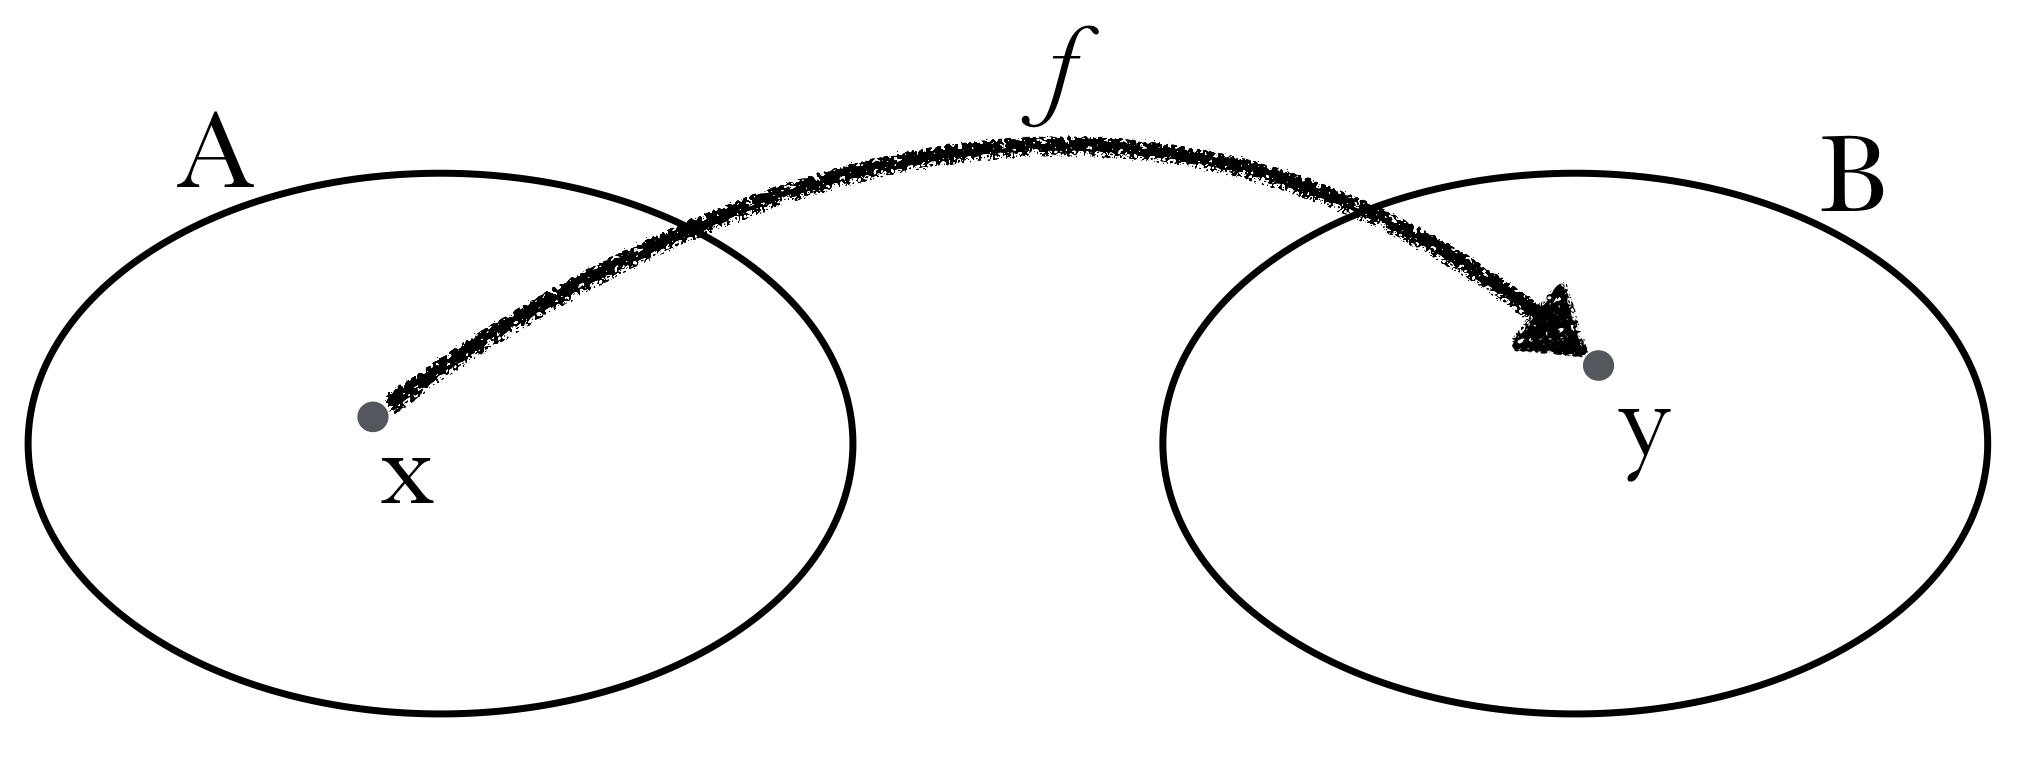
\includegraphics[width=0.55\textwidth]{img/1_funz.png}
  %%\caption{}
  %%\label{fig:1_1}
\end{figure}

Una funzione viene indicata:\\

$f: A\to B  $  tra insiemi   $f: x\mapsto y$   tra elementi  con $x\in A 
$  e $y\in B$\\

Dobbiamo pensare che $x$ mediante la corrispondenza $f$ diventa $y$, 
l'elemento $y$ è dunque l'\textsc{immagine} di $x$ mediante la trasformazione 
$f$; altrettanto e viceversa possiamo chiamare $x$ \textsc{controimmagine} di 
$y$.\\

L'elemento $x$ viene dunque proiettato mediante una sua trasformazione che 
chiamiamo $f$ nell'elemento $y$ di $B$, $y$ risulta così dipendente da $x$ 
perché determinata proprio in funzione di $x$, variabile indipendente.\\

L'immagine $y$ risulta propriamente in funzione di $x$ e possiamo scrivere 
$f(x)=y$ e la precedente espressione tra elementi diventa $f: x\mapsto 
f(x)=y$.\\

Definiamo $D$ \textsc{dominio} l'insieme $A$ delle $x$ e $C$ 
\textsc{codominio} il sottoinsieme di $B$ di tutte le immagini di $x$, cioè 
di tutte e sole le $y$ generate dalla trasformazione $f$.\\

\begin{figure}[htpb!]
  \centering
  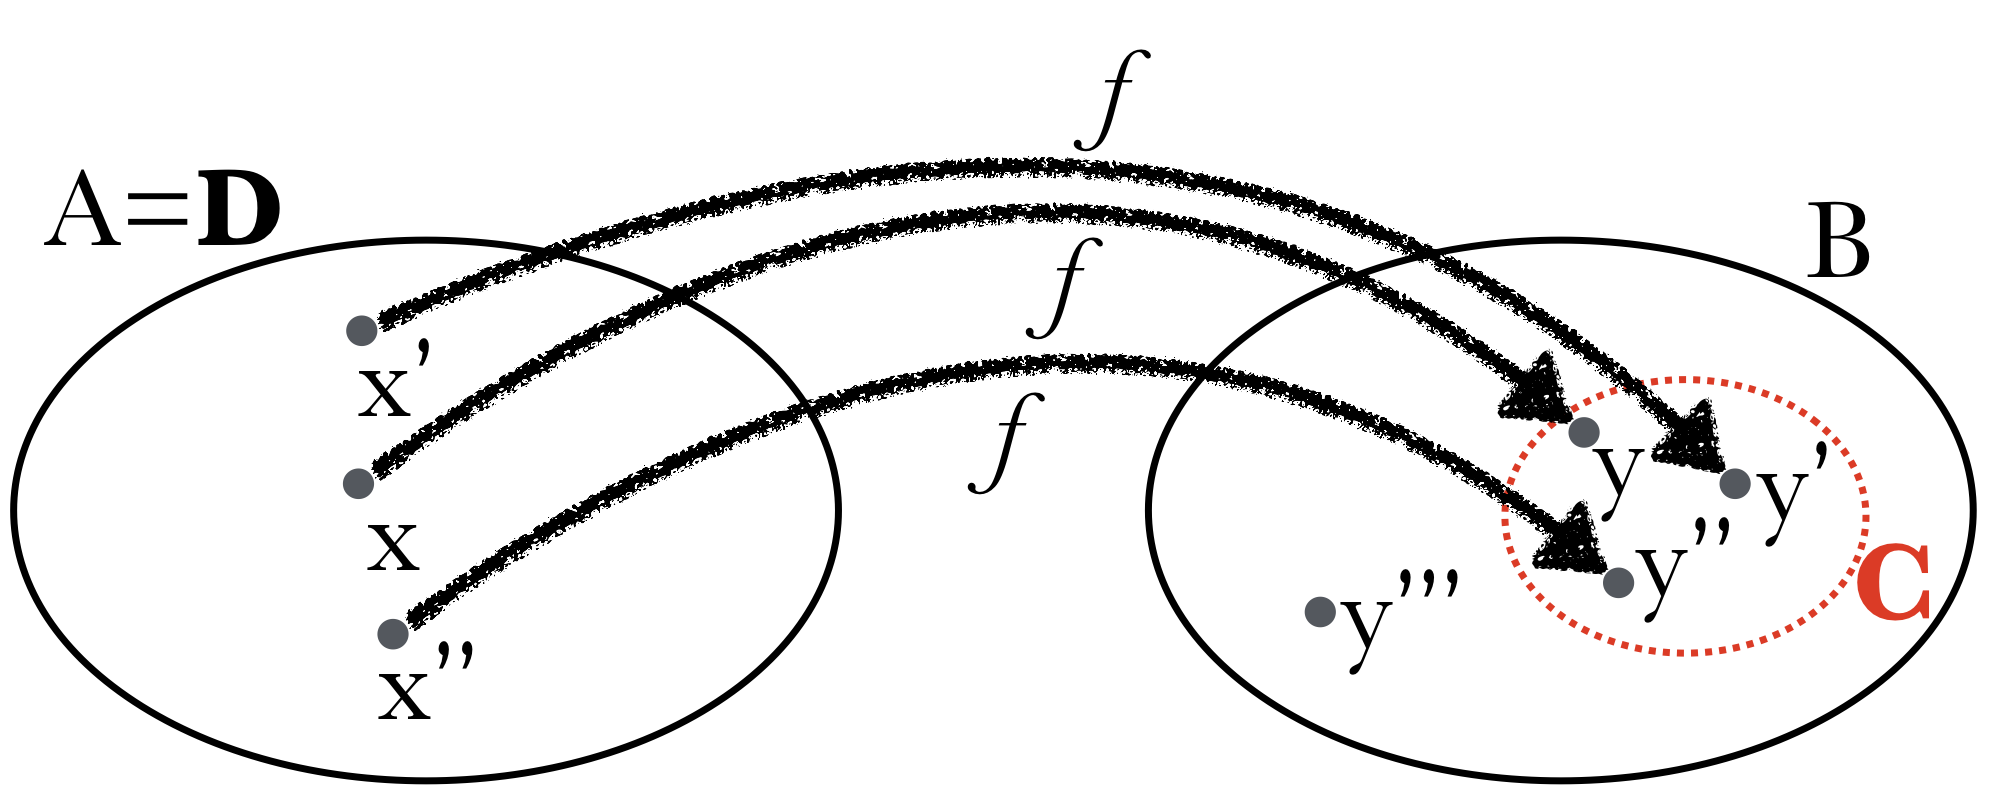
\includegraphics[width=0.55\textwidth]{img/2_funz.png}
  %\caption{}
  %\label{fig:1_2}
\end{figure}
%
Notiamo, nella figura precedente che mentre il dominio coincide con l'insieme 
di partenza il codominio è un sottoinsieme dell'insieme di arrivo.\\

%
%
%
\begin{esempio}
  Visualizziamo dominio e codominio della funzione $f(x)=x^2$
  \begin{figure}[htpb!]
  \centering
  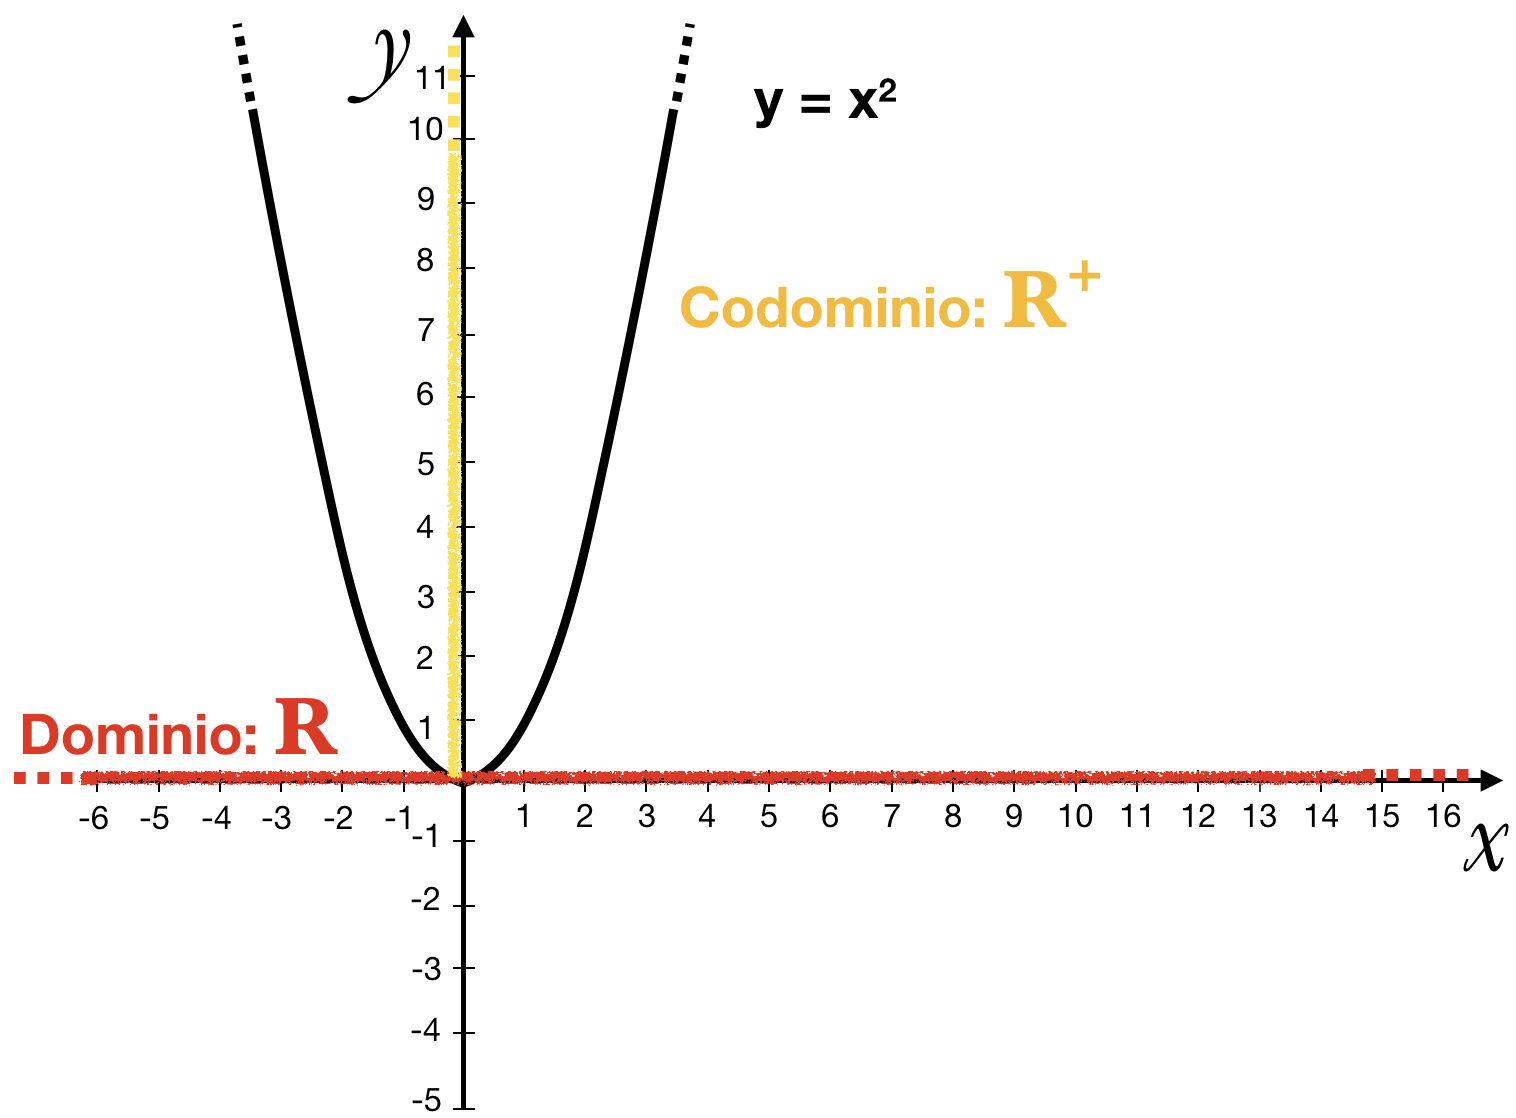
\includegraphics[width=0.4\textwidth]{img/2a_funz.png}
  %\caption{}
  %\label{fig:1_2}
  \end{figure}
\end{esempio}

\begin{esempio}
  Visualizziamo dominio e codominio della funzione $f(x)=\log{x}$
  \begin{figure}[htpb!]
  \centering
  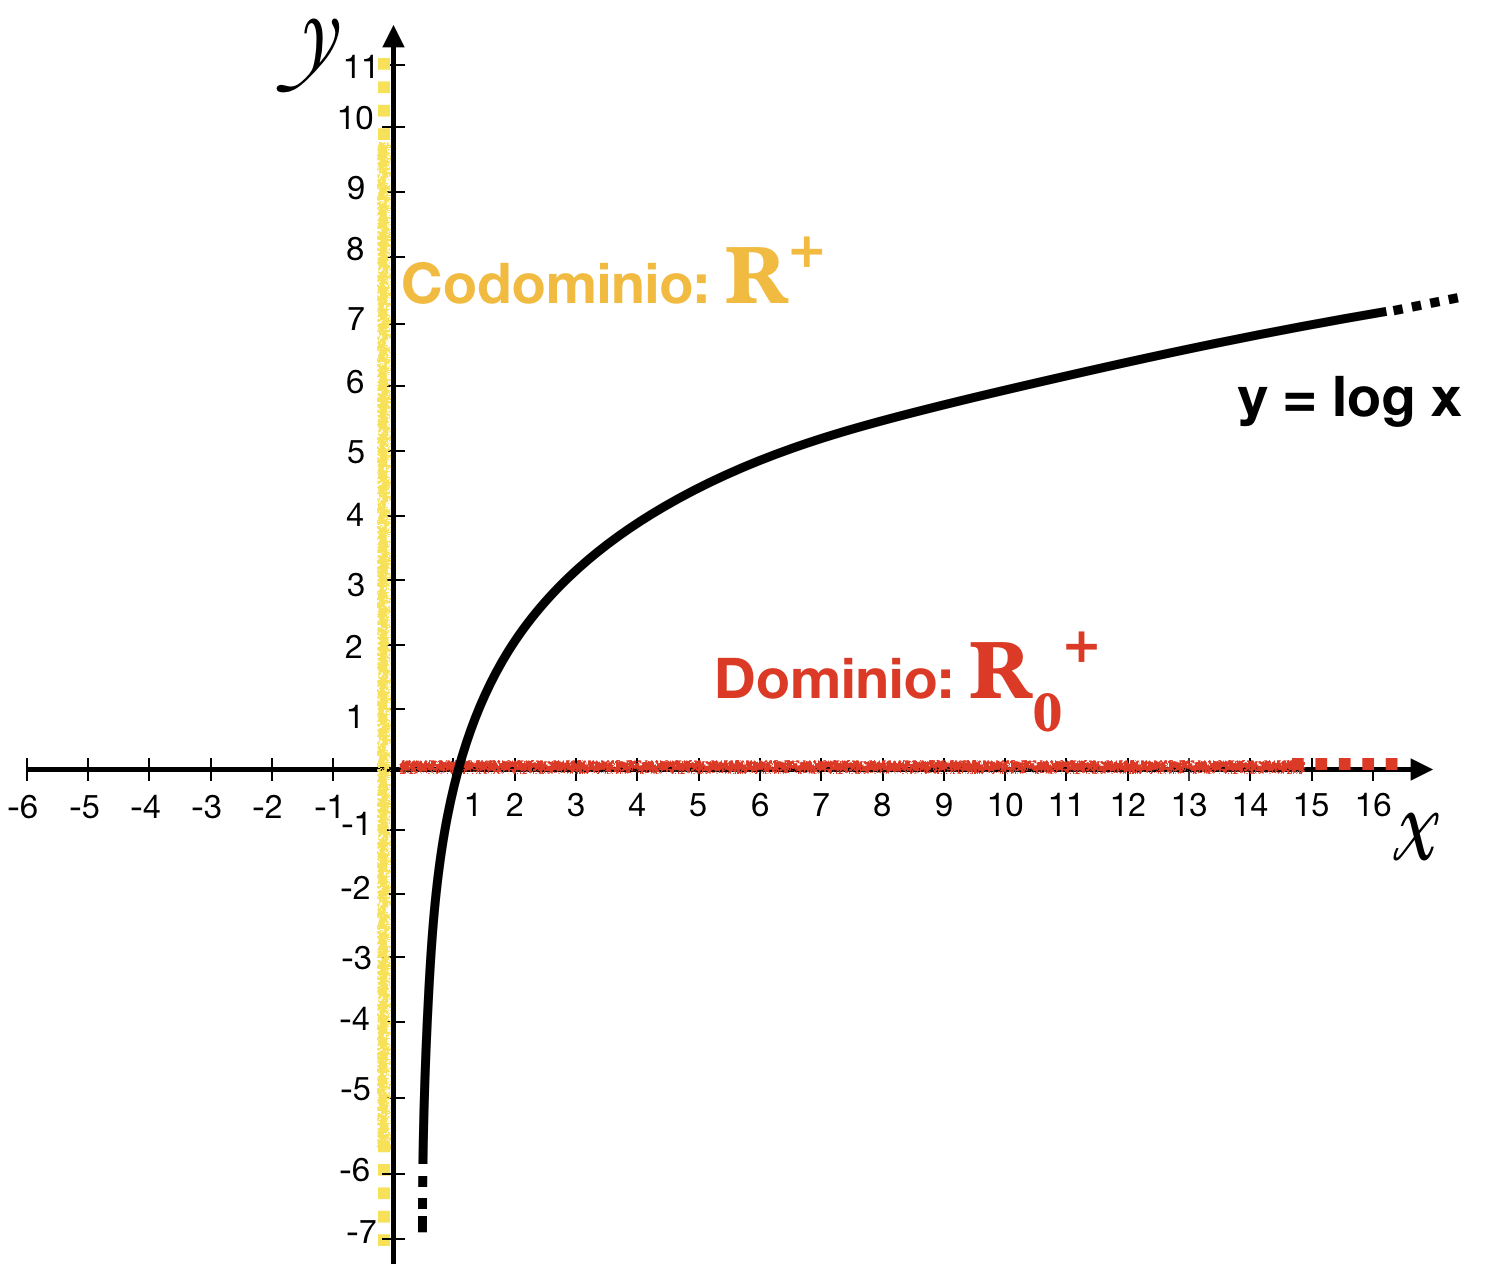
\includegraphics[width=0.4\textwidth]{img/2b_funz.png}
  %\caption{}
  %\label{fig:1_2}
  \end{figure}
\end{esempio}

\begin{esempio}
  Visualizziamo dominio e codominio della funzione $f(x)=\frac{9}{x}$
  \begin{figure}[htpb!]
  \centering
  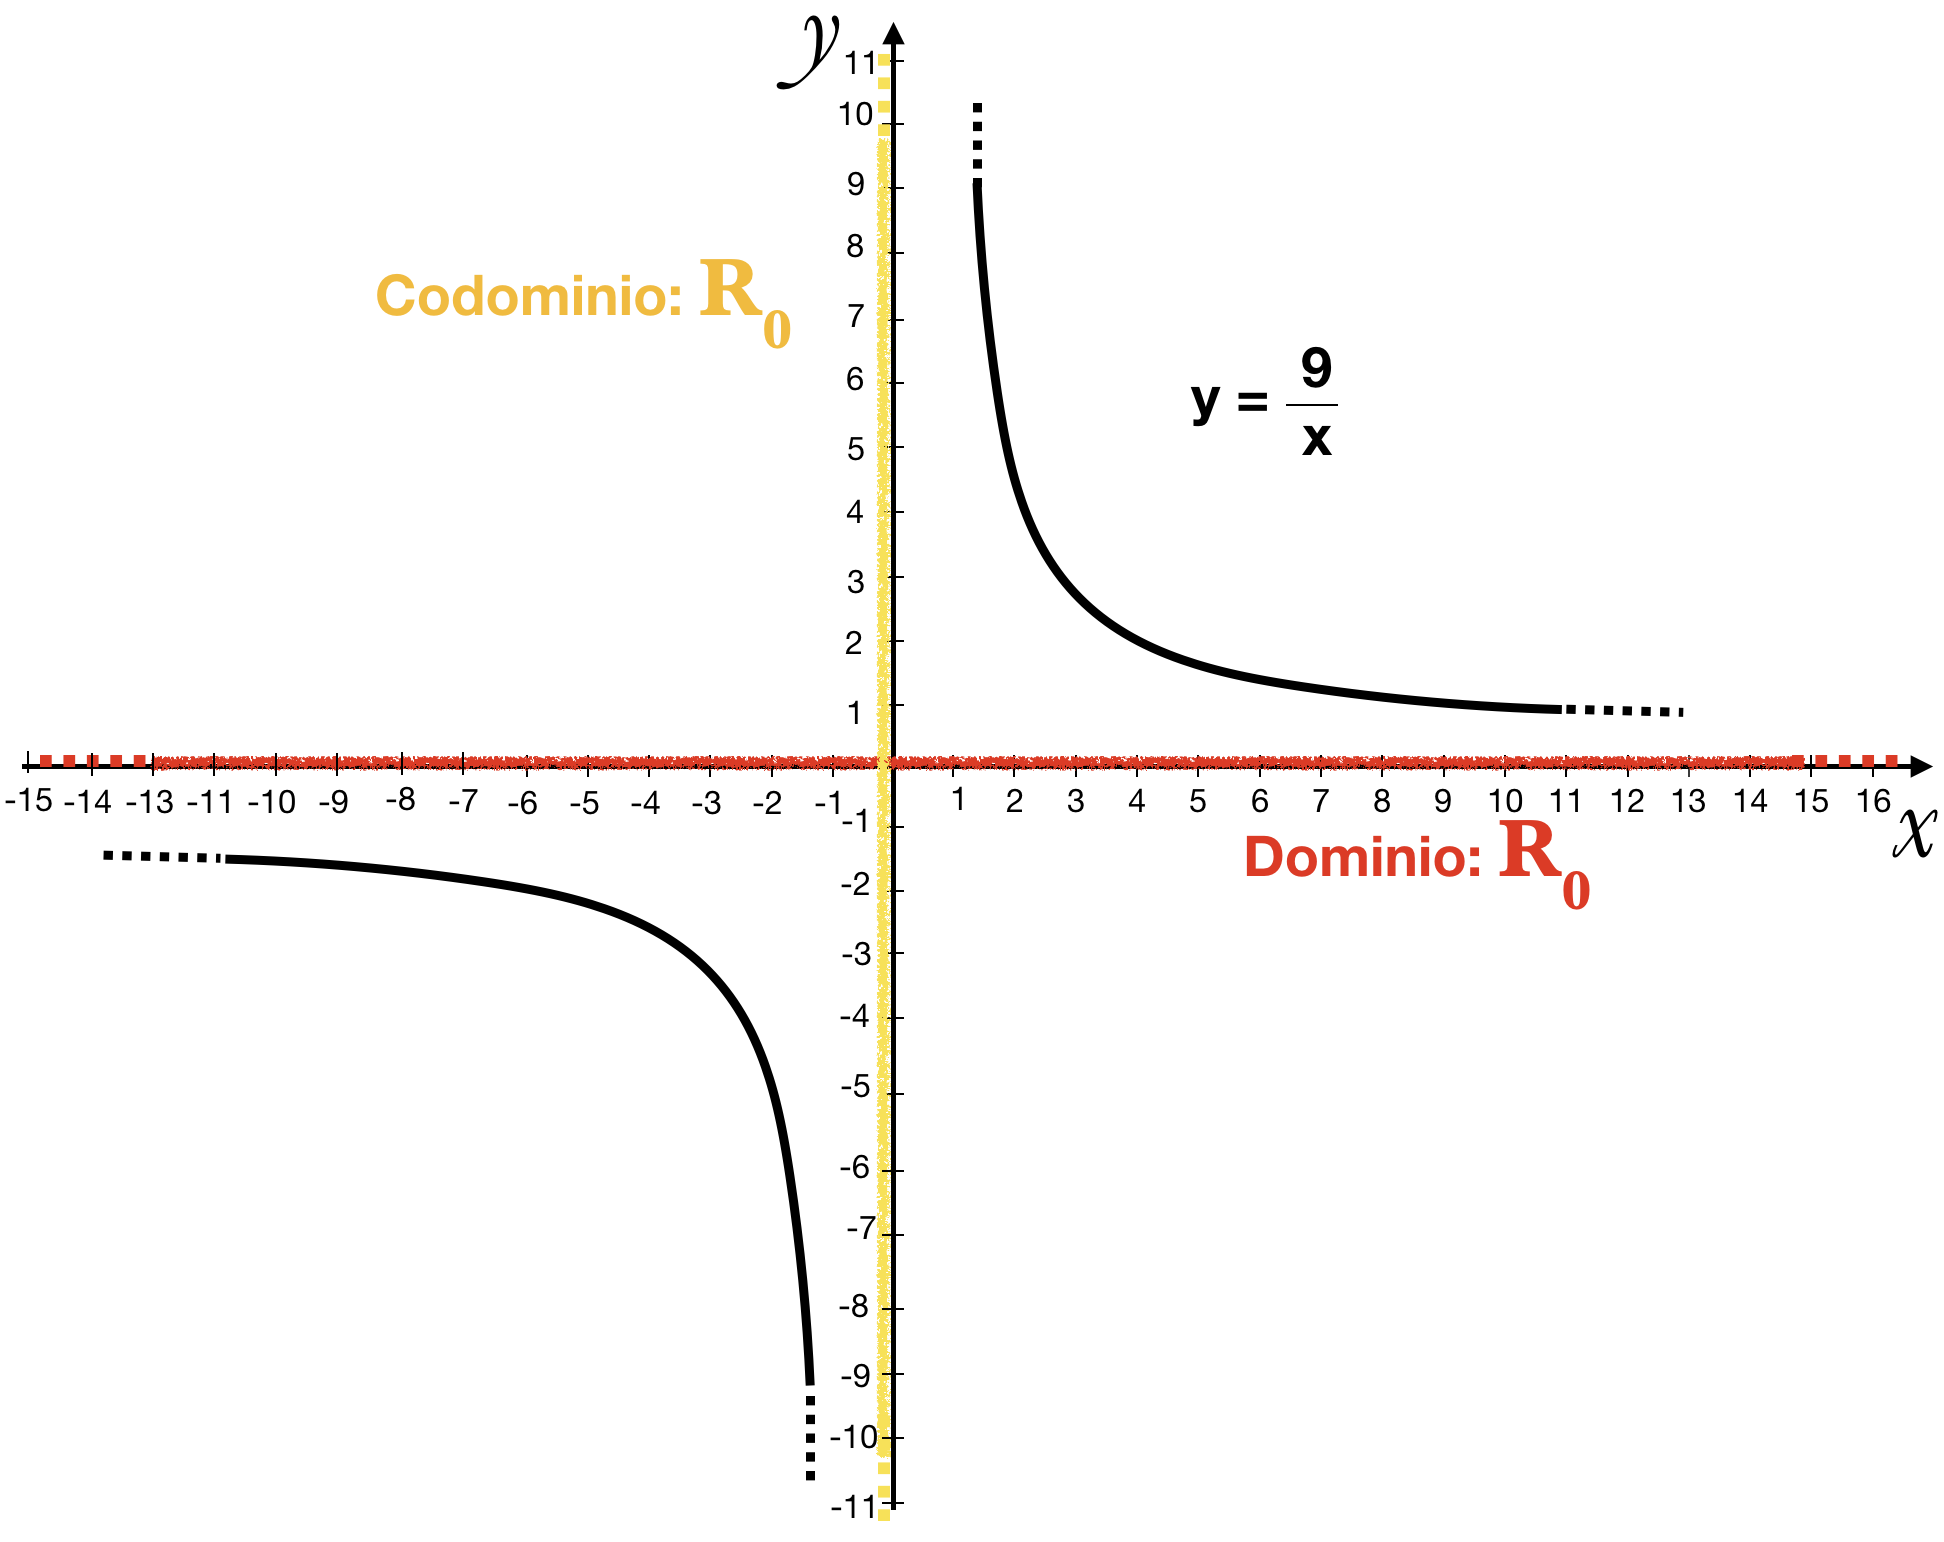
\includegraphics[width=0.55\textwidth]{img/2c_funz.png}
  %\caption{}
  %\label{fig:1_2}
  \end{figure}
\end{esempio}

\newpage 
Per calcolare il dominio delle funzioni, vediamo una tabella riassuntiva dei 
possibili casi.\\

%%%%%%%%%%%%%%TABELLA DOMINIO FUNZIONI%%%%%%%%%%%%
\begin{table}

\raggedleft
  \begin{tabularx}{1,2\textwidth}{XXX}
  \toprule
  Funzione & Dominio  & Esempio \\
  \midrule
  
  \textbf{Funzioni razionali intere} 
\newline$y=a_0x^n+a_1x^{n-1}+\dots+a_n$ 
  & $\,$ \newline $D=\mathbb{R}$ 
  & $\,$ \newline $y=x^3-x^2+2x+1$ \newline $D=\mathbb{R}$ \\
  \midrule

  \textbf{Funzioni razionali fratte} \newline 
$y=\frac{A(x)}{B(x)}$ \newline con $A(x)$ e $B(x)$ polinomi 
  & $\mathbb{R}$ esclusi i valori che annullano $B(x)$, cioè 
\newline $B(x)\neq 0$
  & $\,$ \newline$y=\frac{3+x^2}{x-5}$\newline $D= 
\mathbb{R}-\{5\}$ \\
  \midrule

  \textbf{Funzioni irrazionali} \newline $y=\sqrt[n]{f(x)}$ 
\newline con $n\in\mathbb{N},\,n>1$ 
  & $\,$ \newline Se $n$ è dispari il $D$ è il $D$ di $f(x)$ 
\newline \newline Se $n$ è pari, \newline$D=\{x\in\mathbb{R}\vert f(x)\geq0\}$
  & $\,$ \newline $y=\sqrt[3]{x^2-9}$\newline $D=\mathbb{R}$ 
\newline \newline $y=\sqrt{x^2-1}$\newline $D=x^2\geq1=$\newline 
$=x\leq-1\lor x\geq1$ \\
  \midrule
  
  \textbf{Funzioni logaritmiche} \newline $y=\log_af(x)$ 
\newline con $a>0,\,a\neq1$ \newline \newline $y=\log_{g(x)}(f(x))$ 
  & $\,$ \newline $D=\{x\in\mathbb{R}\vert f(x)>0\}$\newline 
\newline \newline$D=\{x\in\mathbb{R}\vert f(x)>0\land$\newline$\land 
g(x)>0\land g(x)\neq1\}$
  & $\,$ \newline $y=\log(x+1)$\newline $D=x>-1$\\
  \midrule
  
   \textbf{Funzioni esponenziali} \newline $y=a^{f(x)}$ 
\newline con $a>0,\,a\neq1$ \newline\newline  $y={f(x)}^{g(x)}$ 
  & $\,$ \newline $D$ di $f(x)$ \newline \newline \newline 
$D=\{x\in\mathbb{R}\vert f(x)>0\}\land$ $D$ di $g(x)$
  &  $\,$ \newline$y=3^{2x}$\newline $D= \mathbb{R}$ \newline  
\newline$y=e^{\frac{1}{x+1}}$ \newline $D=\mathbb{R}-\{-1\}$ \\
  \midrule
  
  \textbf{Funzioni potenza} \newline $y=f(x)^a$ \newline con 
$a\in\mathbb{R},\,a\neq0$ \newline \newline$a$ intero positivo \newline 
\newline $a$ intero negativo \newline  \newline $a$ razionale \newline  
\newline$a$ irrazionale positivo \newline \newline $a$ irrazionale negativo 
  & $\,$  \newline  \newline  \newline  \newline  $D$ di $f(x)$ 
\newline  \newline $D$ di $f(x)$ con $f(x)\neq0$\newline \newline $D$ di 
$f(x)$ razionale \newline \newline $D=\{x\in\mathbb{R}\vert 
f(x)\geq0\}$\newline \newline $D=\{x\in\mathbb{R}\vert f(x)>0\}$
  & $\,$  \newline  \newline  \newline  \newline $y=(x-1)^2$ 
$D=\mathbb{R}$ \newline \newline $y=(x-1)^{-2}$ $D=x\neq1$ \newline \newline 
$y=(x-1)^{1/2}=\sqrt{x-1}$ $D=x\geq1$ \newline $y=(x-1)^{\pi}$ $D=x\geq1$ 
\newline \newline $y=(x-1)^{-\pi}$ $D=x>1$\\
  \midrule

  \textbf{Funzioni goniometriche} \newline $y=\sin{x}$, 
$y=\cos{x}$ \newline \newline $y=\tan x$, $y=\sec x$ \newline  \newline 
$y=\cot x$, $y=\csc x$ 
  & $\,$ \newline $D=\mathbb{R}$ \newline  \newline 
$D=\mathbb{R} -\bigl\{\frac{\pi}{2}+k\pi \bigr\}$\newline \newline 
$D=\mathbb{R} -\{k\pi\}$
  &  \\
  \midrule
  
\end{tabularx}
\end{table}

\begin{table}   

\raggedleft   
\begin{tabularx}{1,2\textwidth}{XXX}
  \midrule

  \textbf{Funzioni goniometriche inverse} \newline 
$y=\arcsin{x}$, $y=\arccos{x}$ \newline \newline $y=\arctan x$, 
$y=\text{arccot}\,x$
  & $\,$ \newline \newline $D=[-1,1]$ \newline  \newline 
$D=\mathbb{R}$
  &  \\
  \midrule

  \textbf{Funzioni goniometriche composte} \newline 
$y=\sin[f(x)]$, $y=\cos [f(x)]$ \newline \newline $y=\tan [f(x)]$ \newline 
\newline \newline $y=\cot [f(x)]$ \newline  \newline $y=\arcsin[f(x)]$, 
\newline $y=\arccos [f(x)]$ \newline \newline $y=\arctan [f(x)]$
  & $\,$ \newline \newline $D$ di $f(x)$ \newline  \newline 
$D=\bigl\{x\in\mathbb{R}\vert f(x)\neq\frac{\pi}{2}+\newline+k\pi 
\bigr\}$\newline \newline $D=\{x\in\mathbb{R}\vert f(x)\neq k\pi\}$ \newline 
\newline $D=\{x\in\mathbb{R}\vert -1\leq f(x)\leq\newline\leq1\}$ \newline 
\newline $D$ di $f(x)$
  & $\,$ \newline \newline \newline $y=\tan[2x-1]$ \newline 
$2x-1\neq \frac{\pi}{2}+k\pi$ \newline$D=x\neq\frac{\pi+1+k\pi}{2}$  \newline 
\newline \newline  $y=\arcsin[x-1]$ \newline $-1\leq x-1\leq1$\newline $0\leq 
x\leq2$\newline \newline$y=\arctan [\frac{x+2}{x+3}]$ \newline 
$D=\mathbb{R}-\{-3\}$
 \\

  \bottomrule
\end{tabularx}
\end{table}
\newpage

\section{La rappresentazione di una funzione}
%label{}
Una funzione può essere rappresentata in diversi modi, i principali sono:
\begin{itemize}
  \item \textsc{Rappresentazione tabulare}\\
Le funzioni empiriche vengono ricostruite con una tabella in cui ad ogni $y$ 
corrisponde un certo $x$. Ad esempio pensiamo ad una tabella che dà la 
temperatura ora per ora in un certo luogo.
%
  \item \textsc{Rappresentazione analitica}\\
La funzione è espressa mediante un insieme di operazioni matematiche che 
applicate in un certo ordine ad $x$ restituiscono un corrispondente valore di 
$y$. Esempi ne sono $y=\log{(x+2)}$, $y=2x^3+3$ o $y=\sin{x}+2^x$, cioè le 
espressioni, scritte in linguaggio matematico, che siamo abituati a trattare.
%
  \item \textsc{Rappresentazione grafica}\\
La funzione è rappresentata come una corrispondenza $x-$y su un grafico 
cartesiano; in particolare, ricordiamo che: il grafico di una funzione $f 
:A\to B$ è l'insieme di tutte le coppie ordinate $(x;y)$ che si ottengono 
prendendo un valore $x$ in $A$ e trovando il corrispondente valore $y=f(x)$ 
in $B$. Ogni coppia ordinata rappresenta un punto nel piano cartesiano 
$\mathbb{R}^2$.
\end{itemize}

\section{Le proprietà di una funzione}
%label{}
Una funzione, a seconda, del modo in cui gli elementi del dominio 
corrispondono agli elementi del codominio si può definire \textsc{iniettiva}, 
\textsc{suriettiva} e \textsc{biiettiva} (o \textsc{biunivoca}).\\

\begin{definizione}
Una funzione da $A$ a $B$ si dice \textsc{iniettiva} se ogni elemento di $B$ 
è immagine di \underline{al più} un elemento di $A$;\\


$f : A\to B$ è iniettiva se  $\forall x_1,\,x_2\in A ,\,x_1\neq 
x_2\Rightarrow f(x_1 )\neq f(x_2)$
\end{definizione}

\begin{figure}[htpb!]
  \centering
  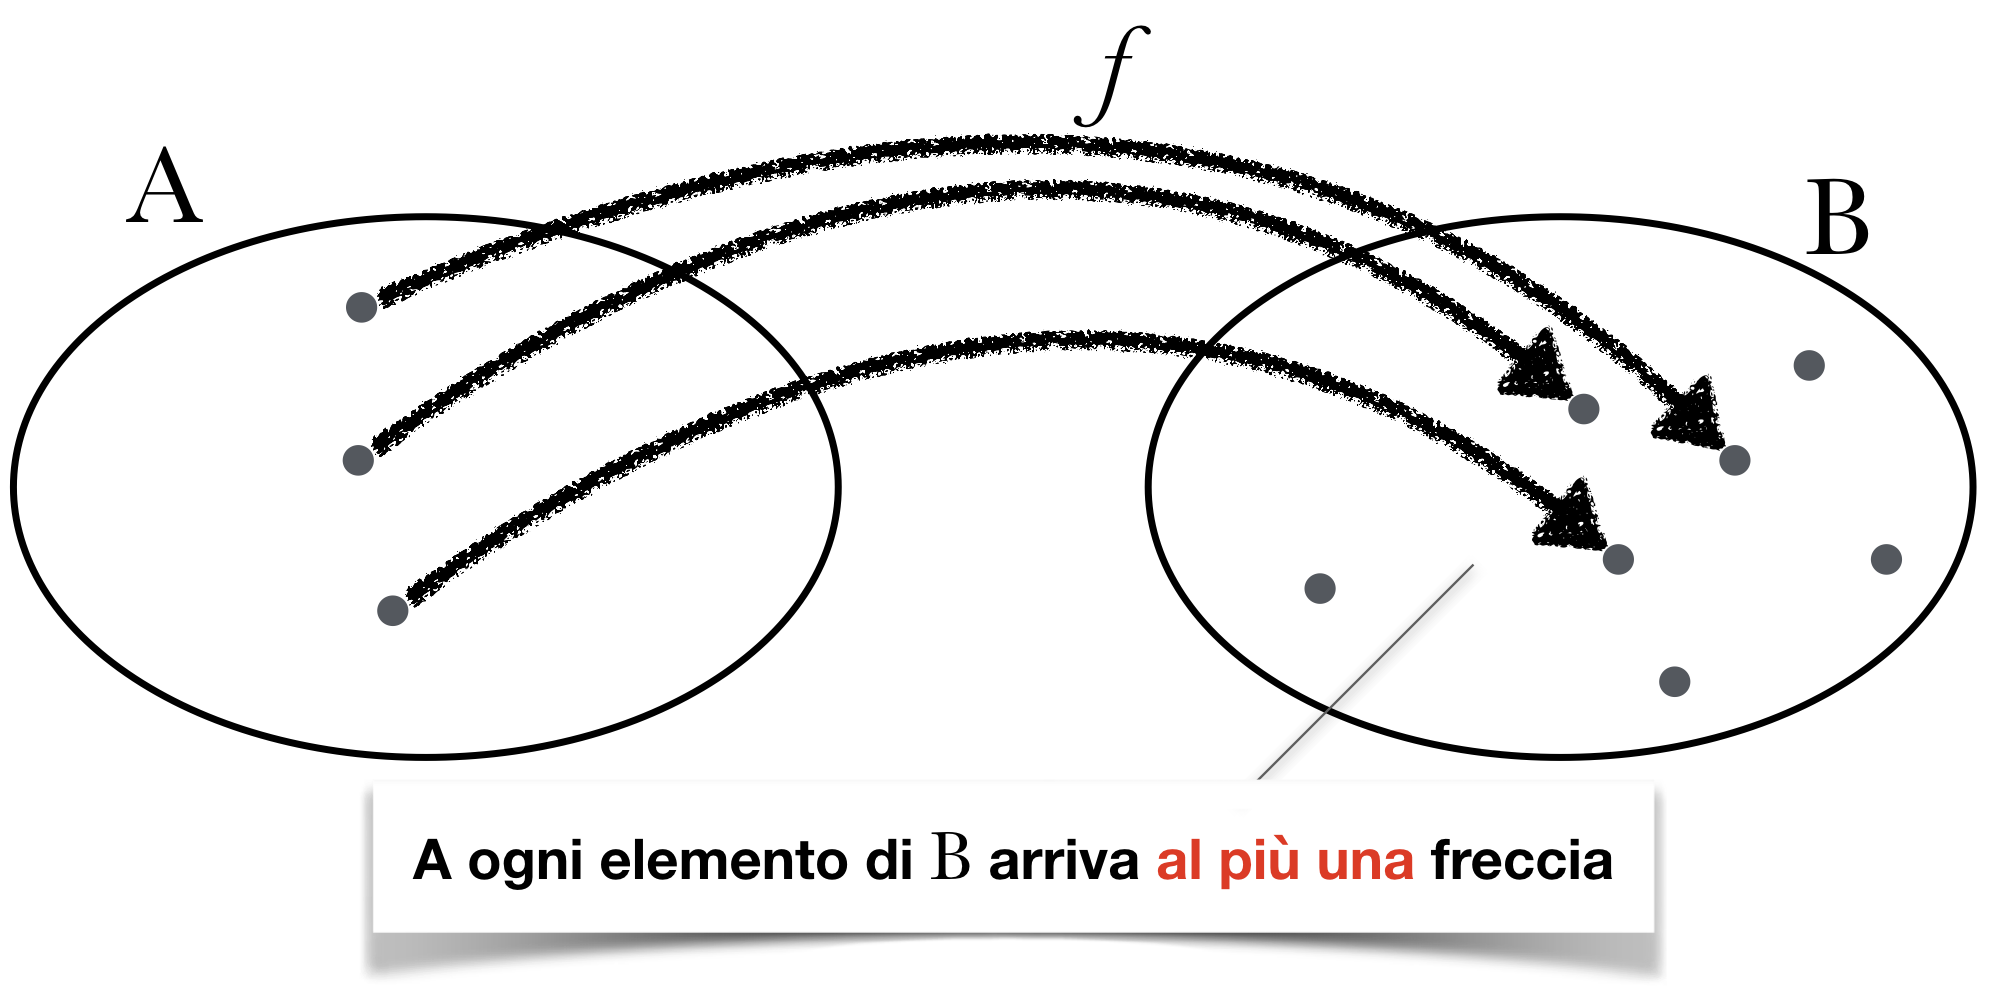
\includegraphics[width=0.55\textwidth]{img/3_funz.png}
  %\caption{}
  %\label{fig:1_2}
\end{figure}

\begin{definizione}
Una funzione da $A$ a $B$ si dice \textsc{suriettiva} quando ogni elemento di 
$B$ è immagine di \underline{almeno un} elemento di $A$;\\

$f: A\to B$ è suriettiva se $\forall y\in B, \exists x\in A \mid f(x)=y$
\end{definizione}

\begin{figure}[htpb!]
  \centering
  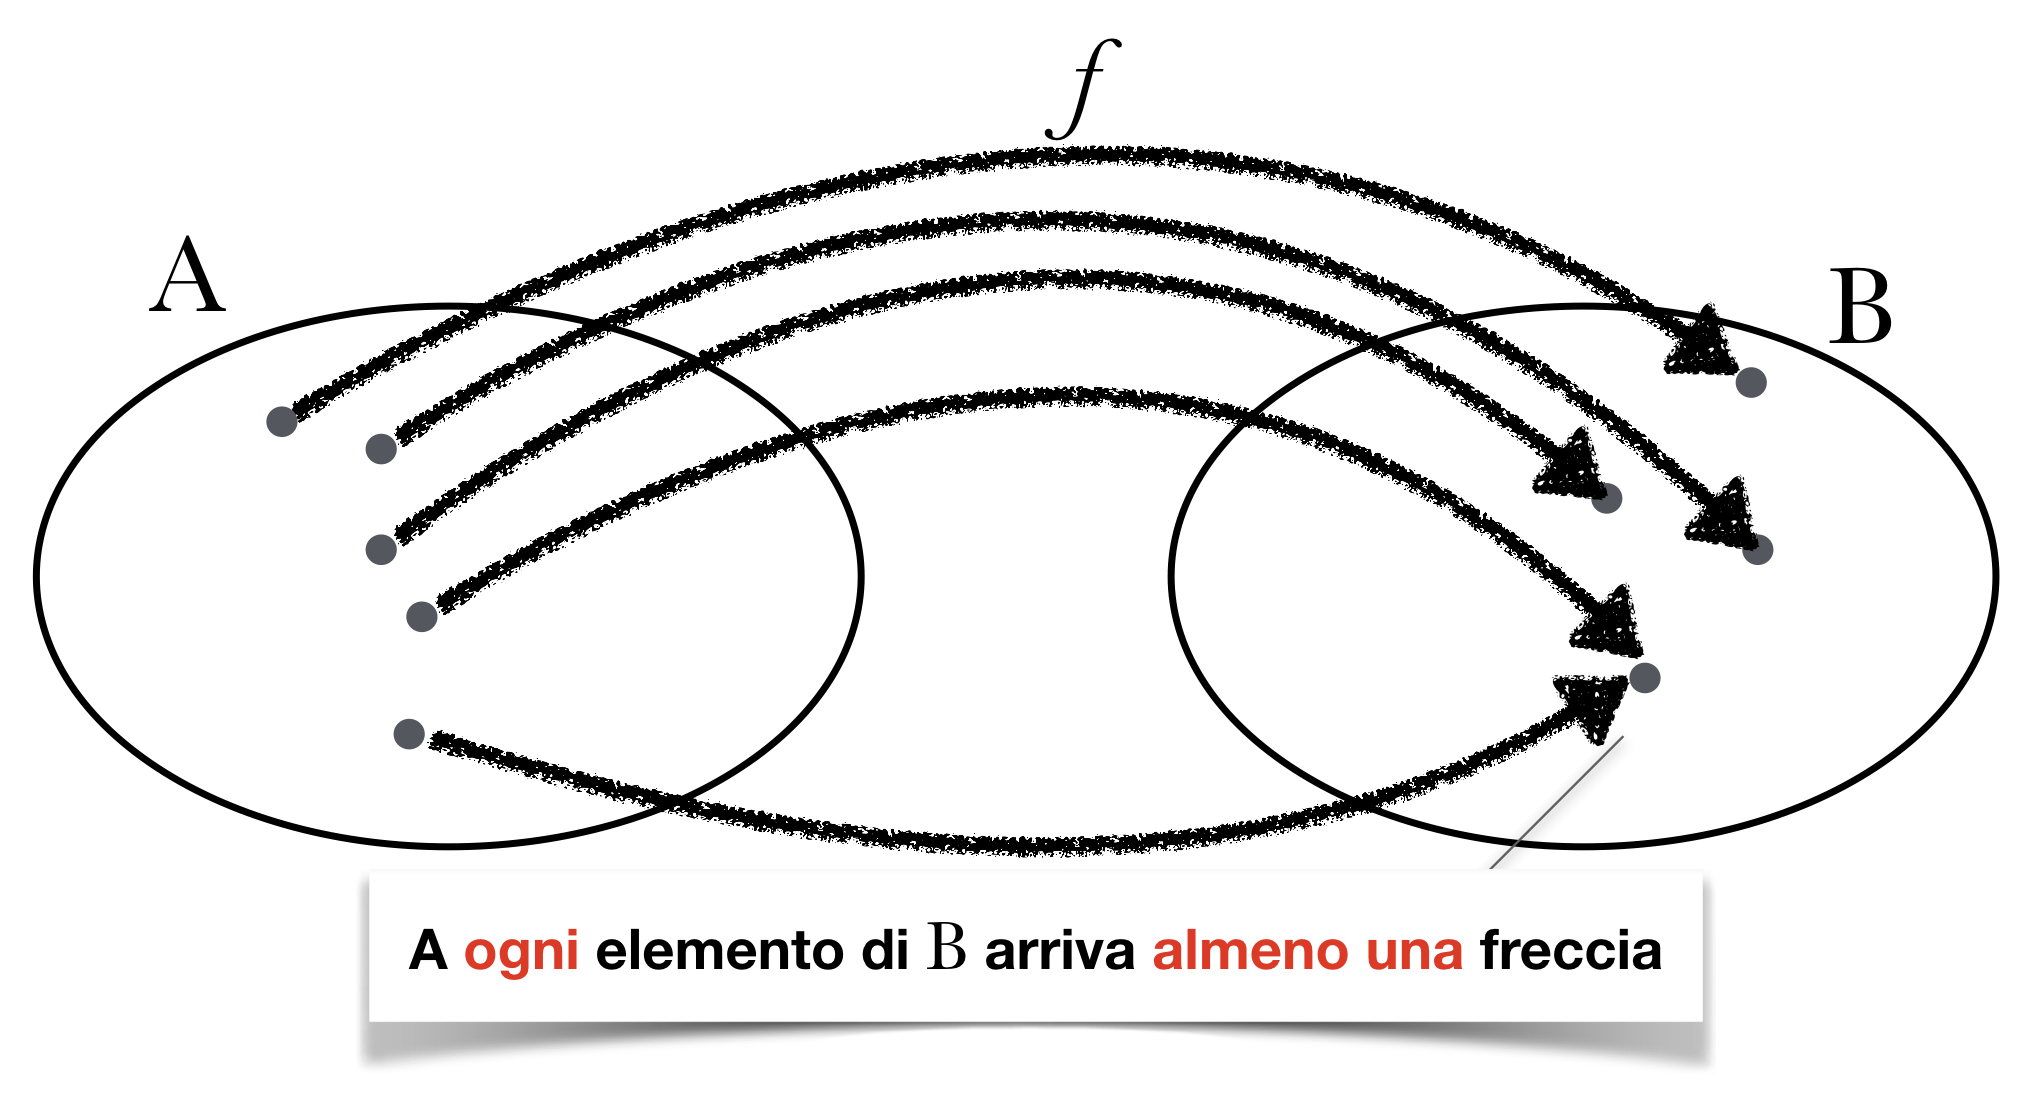
\includegraphics[width=0.55\textwidth]{img/4_funz.png}
  %\caption{}
  %\label{fig:1_2}
\end{figure}

Il fatto che una funzione sia o non sia suriettiva dipende da come si sceglie 
l'insieme di arrivo. Se lo si sceglie coincidente con il codominio la 
funzione è suriettiva.\\
%
\begin{definizione}
Una funzione da $A$ a $B$ è \textsc{biiettiva} (o \textsc{biunivoca}) quando 
è sia iniettiva sia suriettiva.\\
\end{definizione}

\begin{figure}[htpb!]
  \centering
  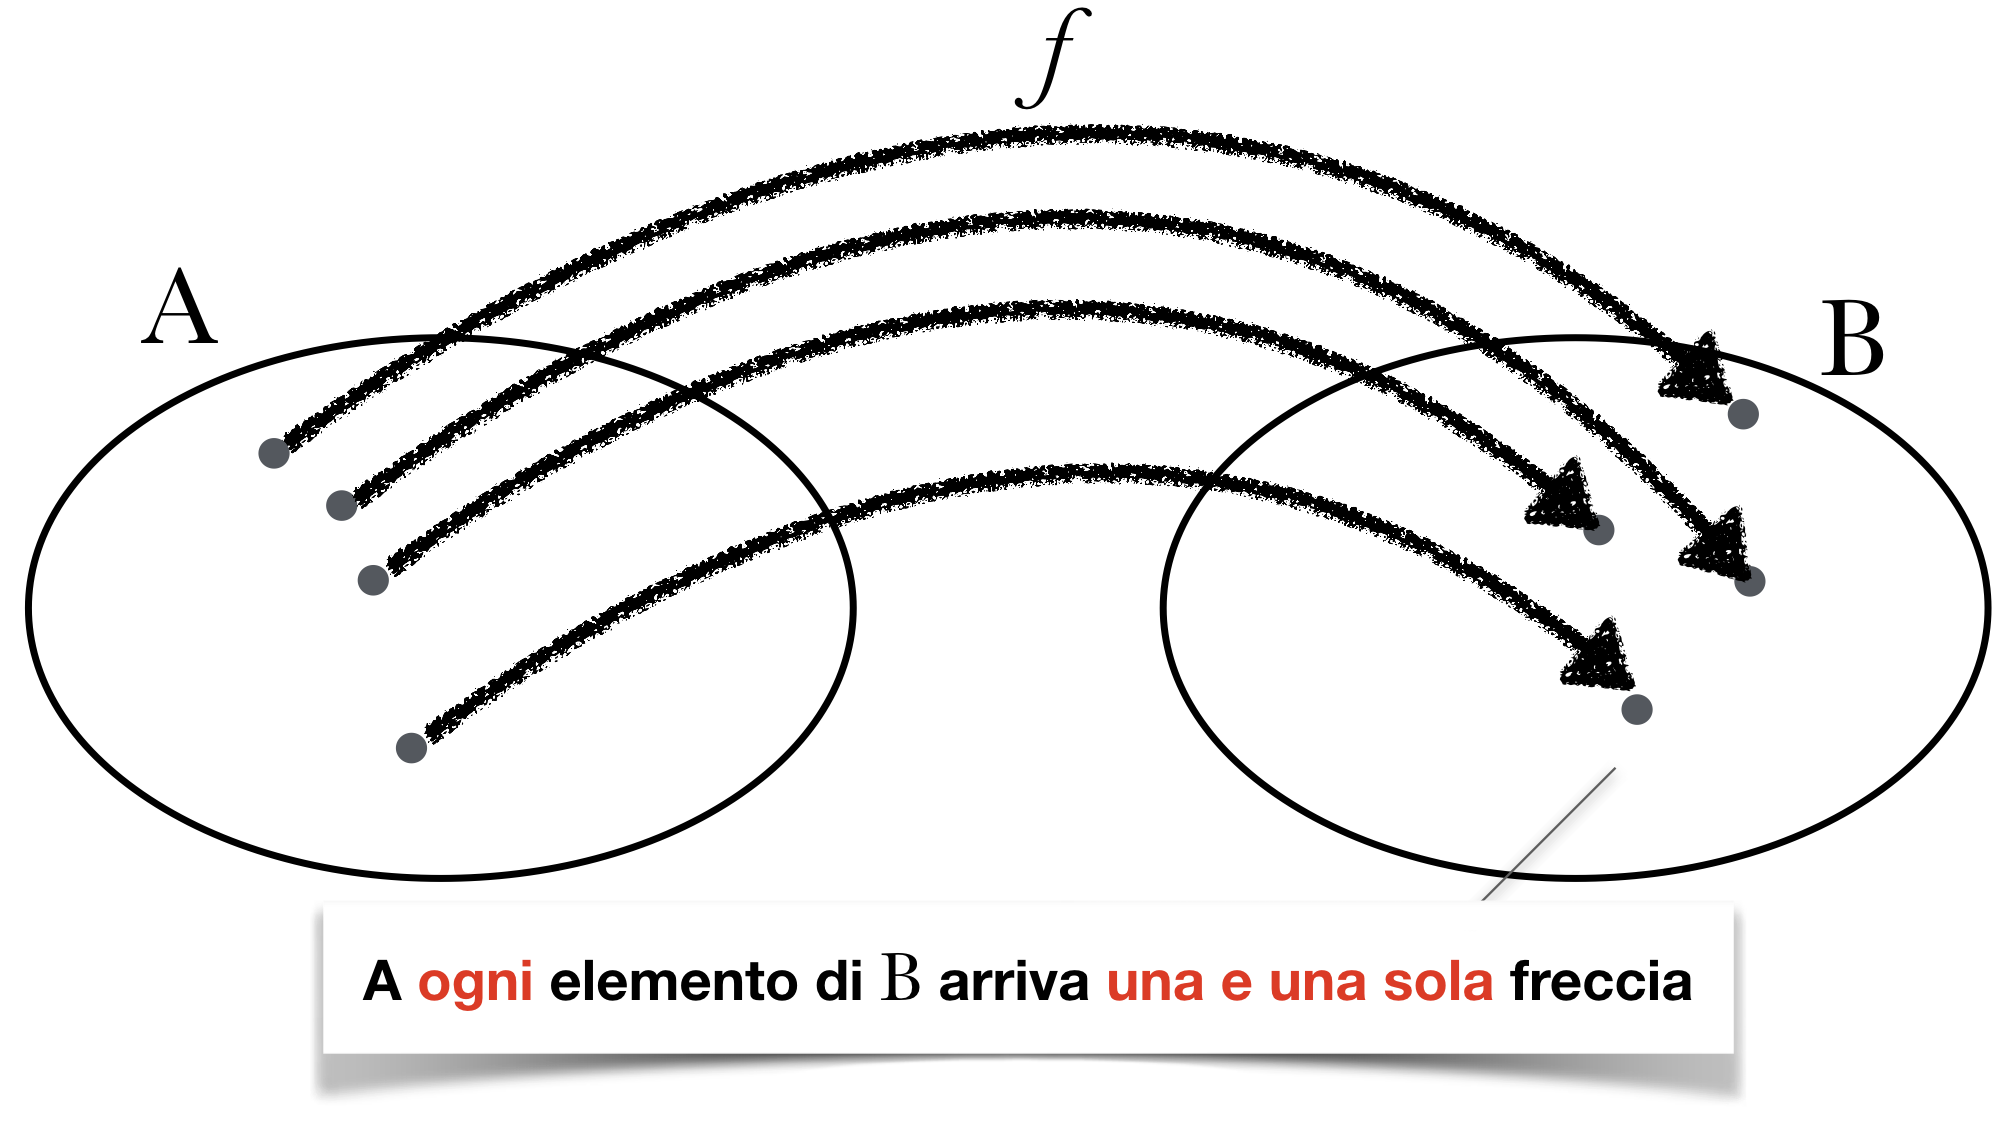
\includegraphics[width=0.55\textwidth]{img/5_funz.png}
  %\caption{}
  %\label{fig:1_2}
\end{figure}

\begin{esempio} Quando una funzione è biettiva?\\
Una funzione biiettiva è ad esempio una qualsiasi retta. Una retta è infatti 
sia iniettiva, che biettiva di dominio $\mathbb{R}$ e codominio 
$\mathbb{R}$.\\
\end{esempio}

Una funzione biiettiva viene anche detta biiezione o corrispondenza biunivoca 
fra gli insieme $A$ e $B$. Tale relazione tra insiemi è molto forte e 
specifica in quanto ad ogni elemento di $A$ viene associato un solo elemento 
di $B$ e, reciprocamente, ad ogni elemento di $B$ è associato un solo 
elemento di $A$, in una relazione uno a uno. Per tale ragione, la relazione 
tra i due insiemi viene indicata con una doppia freccia $A\leftrightarrow B$.
%
\section{Le caratteristiche di una funzione}
%label{}
Analizziamo ora le caratteristiche che può manifestare una funzione, qualità 
che può presentare il suo andamento e che possono contraddistinguerne la 
forma del grafico.

\subsection{Monotonia}
%label{}
La caratteristica della monotonia vuole evidenziare l'andamento 
\textsc{crescente} o \textsc{decrescente} di una funzione; la monotonia 
studia il comportamento della variabile dipendente $y$ all'aumentare della 
variabile indipendente $x$. All'aumentare dell'ascissa se aumenta anche 
l'ordinata diremo che la funzione cresce, se l'ordinata diminuisce diremo che 
la funzione decresce. Vediamo e puntualizziamo meglio.\\

\begin{definizione}
Una funzione $y=f(x)$ di dominio $D$, si dice \textsc{crescente in senso 
stretto} in un intervallo $I$, sottoinsieme di $D$, se\\

$\forall x_1,x_2\in I$  con $x_1<x_2 $ si ha $f(x_1)<f(x_2)$\\
\end{definizione}

\begin{figure}[htpb!]
  \centering
  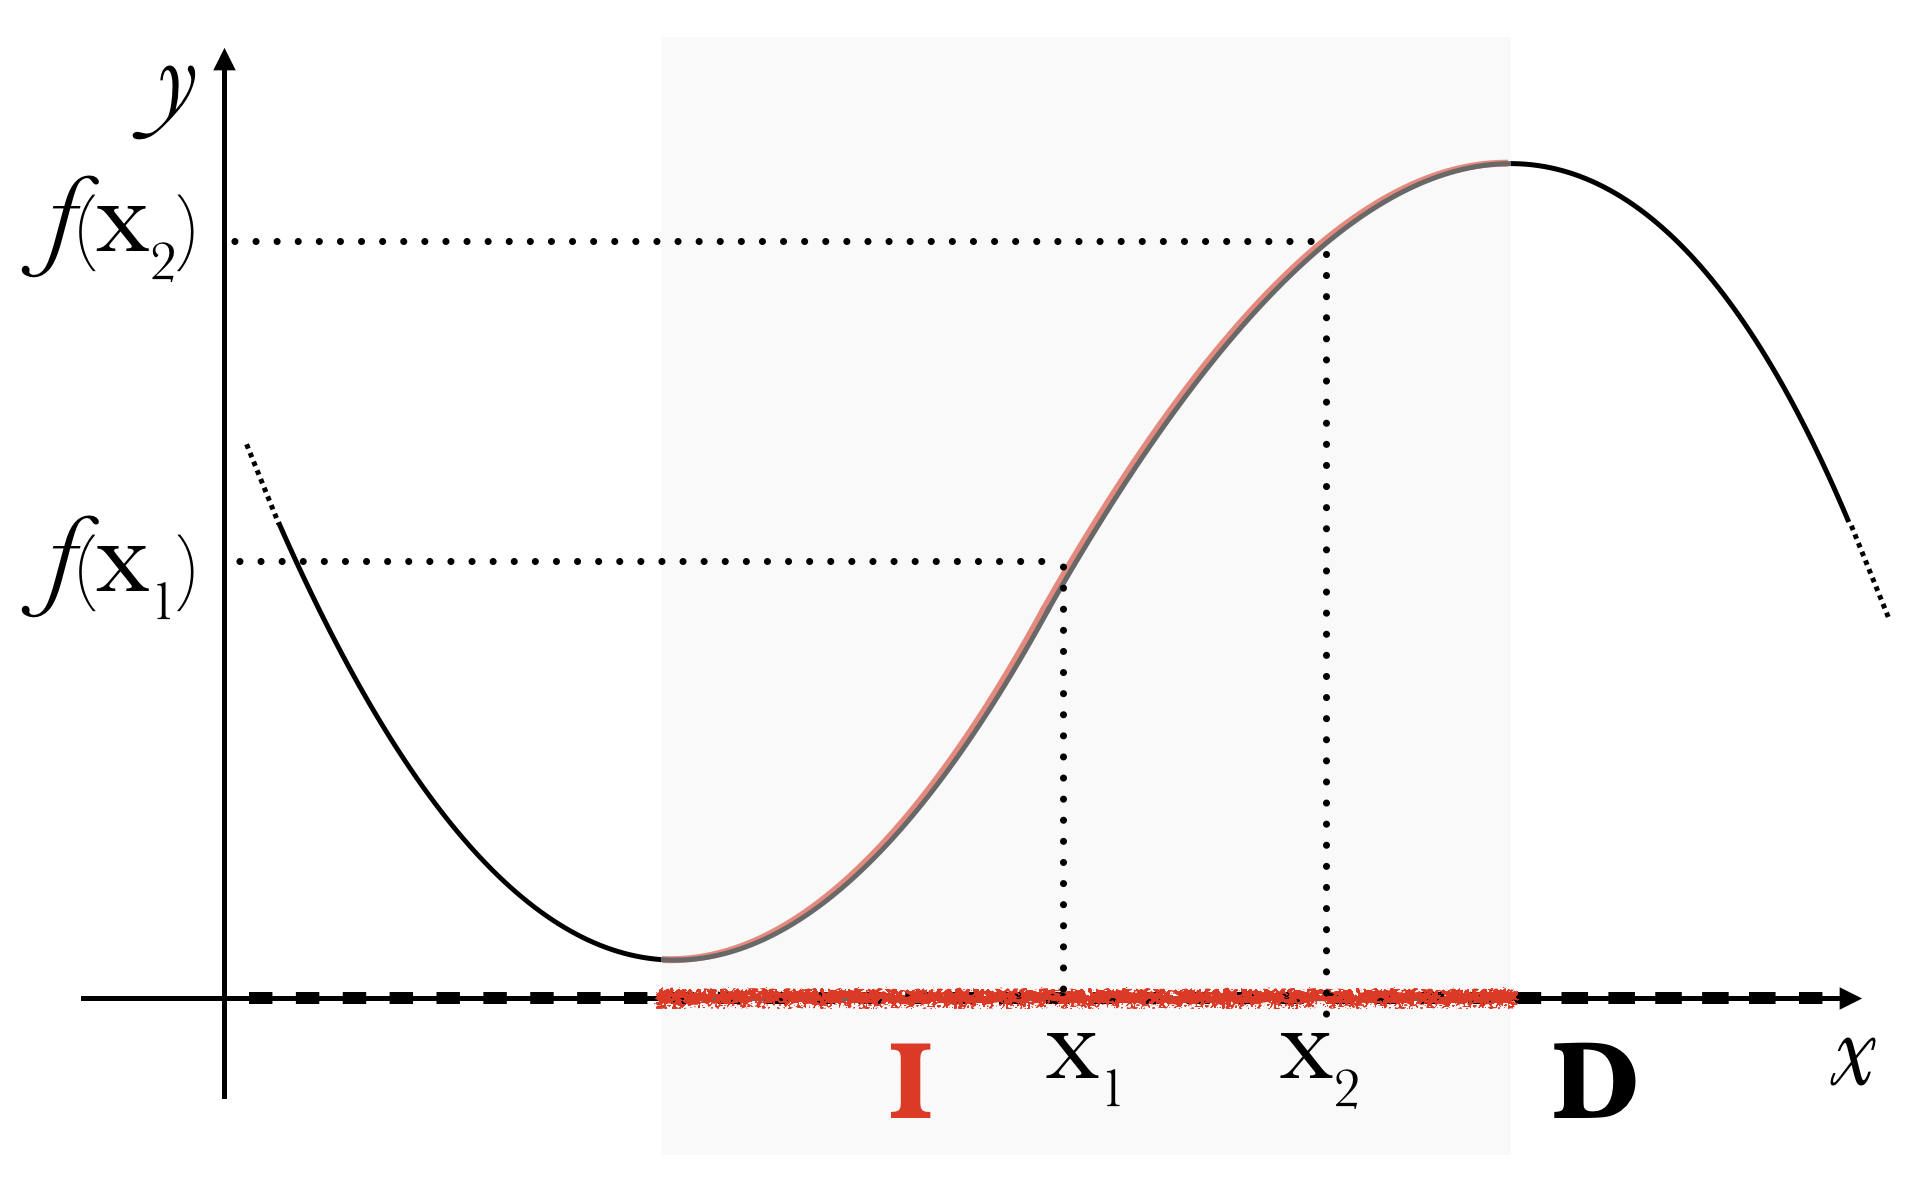
\includegraphics[width=0.55\textwidth]{img/funz_6.png}
  %\caption{}
  %\label{fig:1_2}
\end{figure}
%
\begin{definizione}
Una funzione è non decrescente o \textsc{crescente} in senso lato in un 
intervallo $I$, sottoinsieme di $D$, se\\

$\forall x_1,x_2\in I$  con $x_1<x_2 $ si ha $f(x_1)\leq f(x_2)$\\
%
\end{definizione}
%
%
%

\begin{definizione}
Una funzione $y=f(x)$ di dominio $D$, si dice \textsc{decrescente in senso 
stretto}, in un intervallo $I$, sottoinsieme di $D$, se\\

$\forall x_1,x_2\in I$  con $x_1<x_2 $ si ha $f(x_1)> f(x_2)$\\

\end{definizione}

\begin{figure}[htpb!]
  \centering
  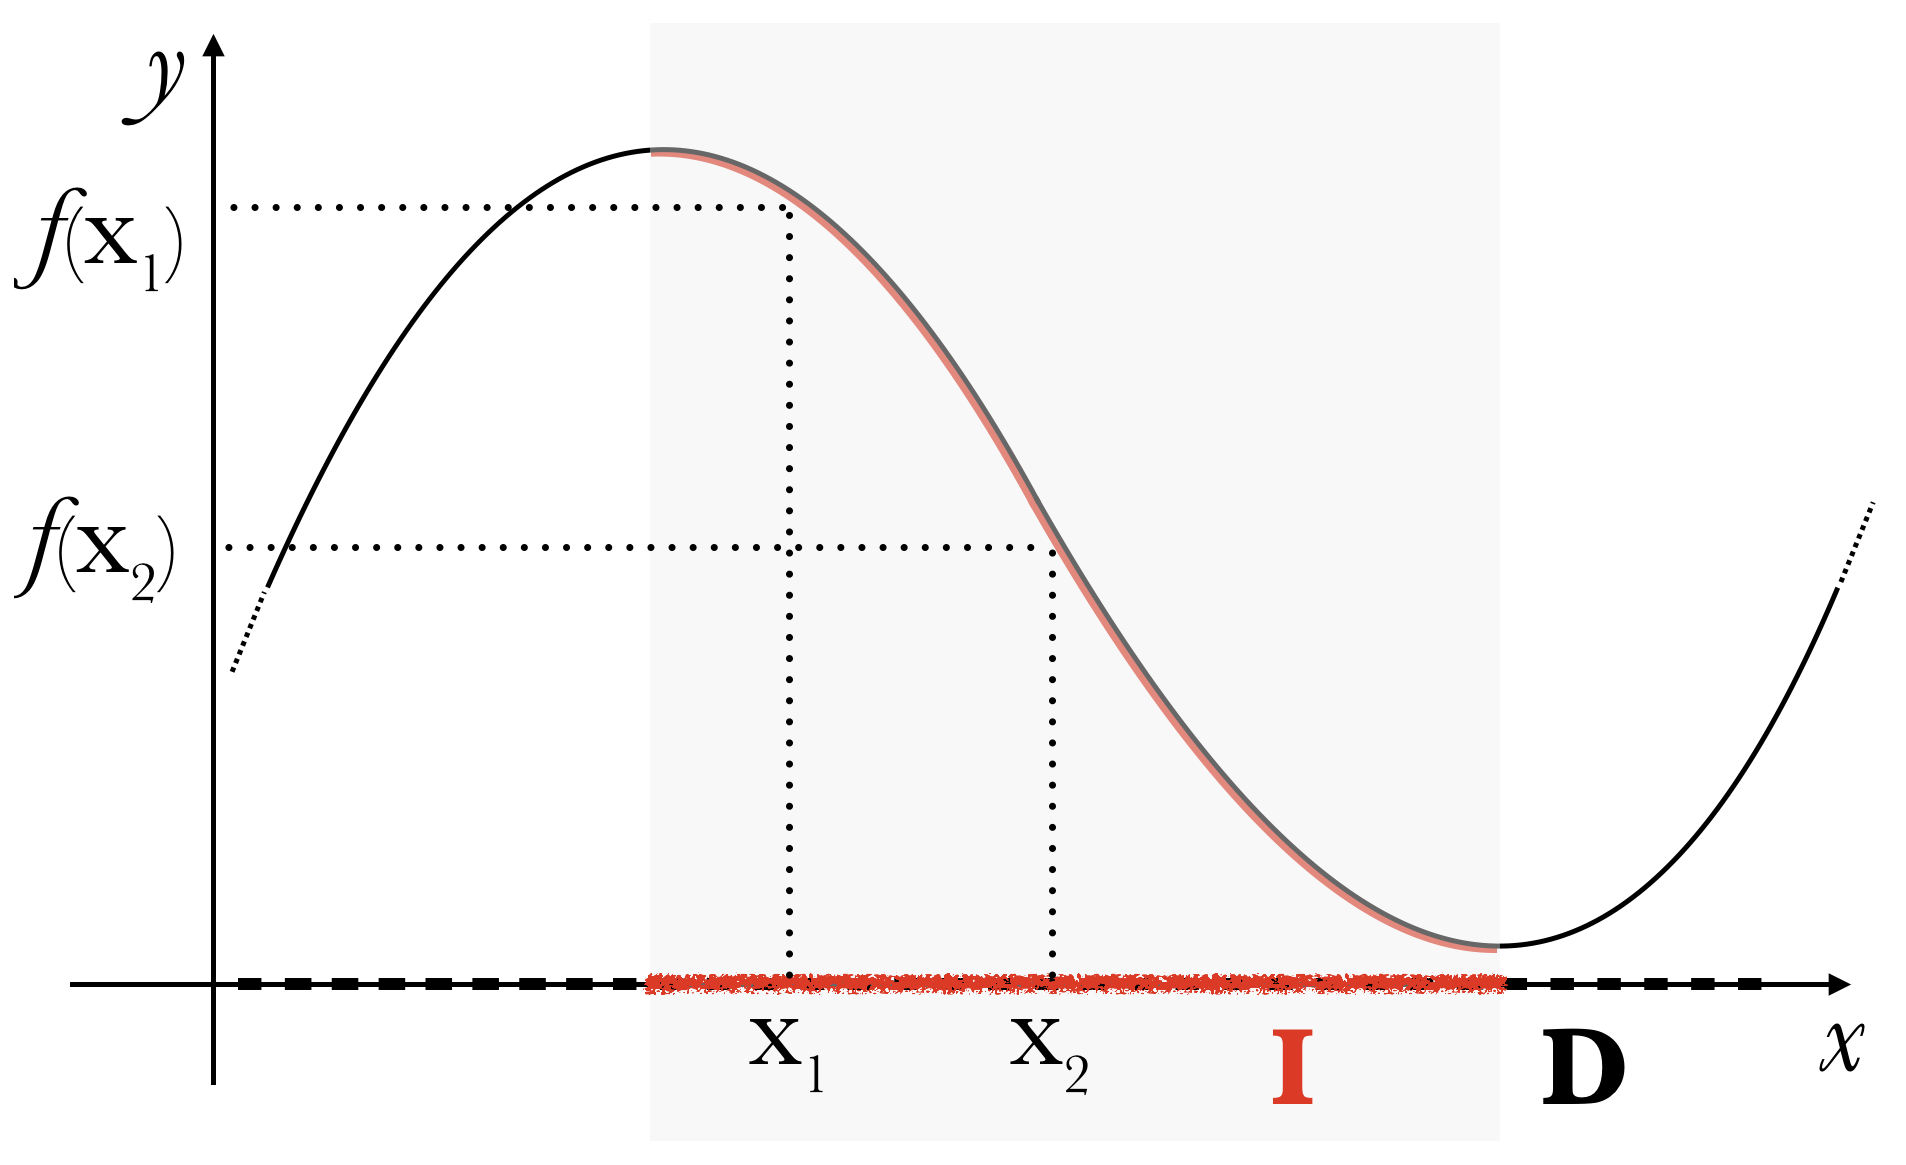
\includegraphics[width=0.55\textwidth]{img/funz_7.png}
  %\caption{}
  %\label{fig:1_2}
\end{figure}
%

\begin{definizione}
Una funzione è non crescente o \textsc{decrescente} in senso lato in un 
intervallo $I$, sottoinsieme di $D$, se\\

$\forall x_1,x_2\in I$  con $x_1<x_2 $ si ha $f(x_1)\geq f(x_2)$\\
\end{definizione}

Una funzione, quindi, si dice monotòna in un intervallo $I$ del suo dominio 
se in $I$ è sempre crescente o decrescente.\\

\begin{esempio}
Individuiamo gli intervalli in cui la funzione rappresentata risulta 
crescente o decrescente.\\
Negli intervalli finiti $x_1<x<x_2$, $x_3<x<x_4$ la funzione risulta essere 
crescente; negli intervalli finiti $x_2<x<x_3$, $x_4<x<x_5$.
% 
\begin{figure}[htpb!]
  \centering
  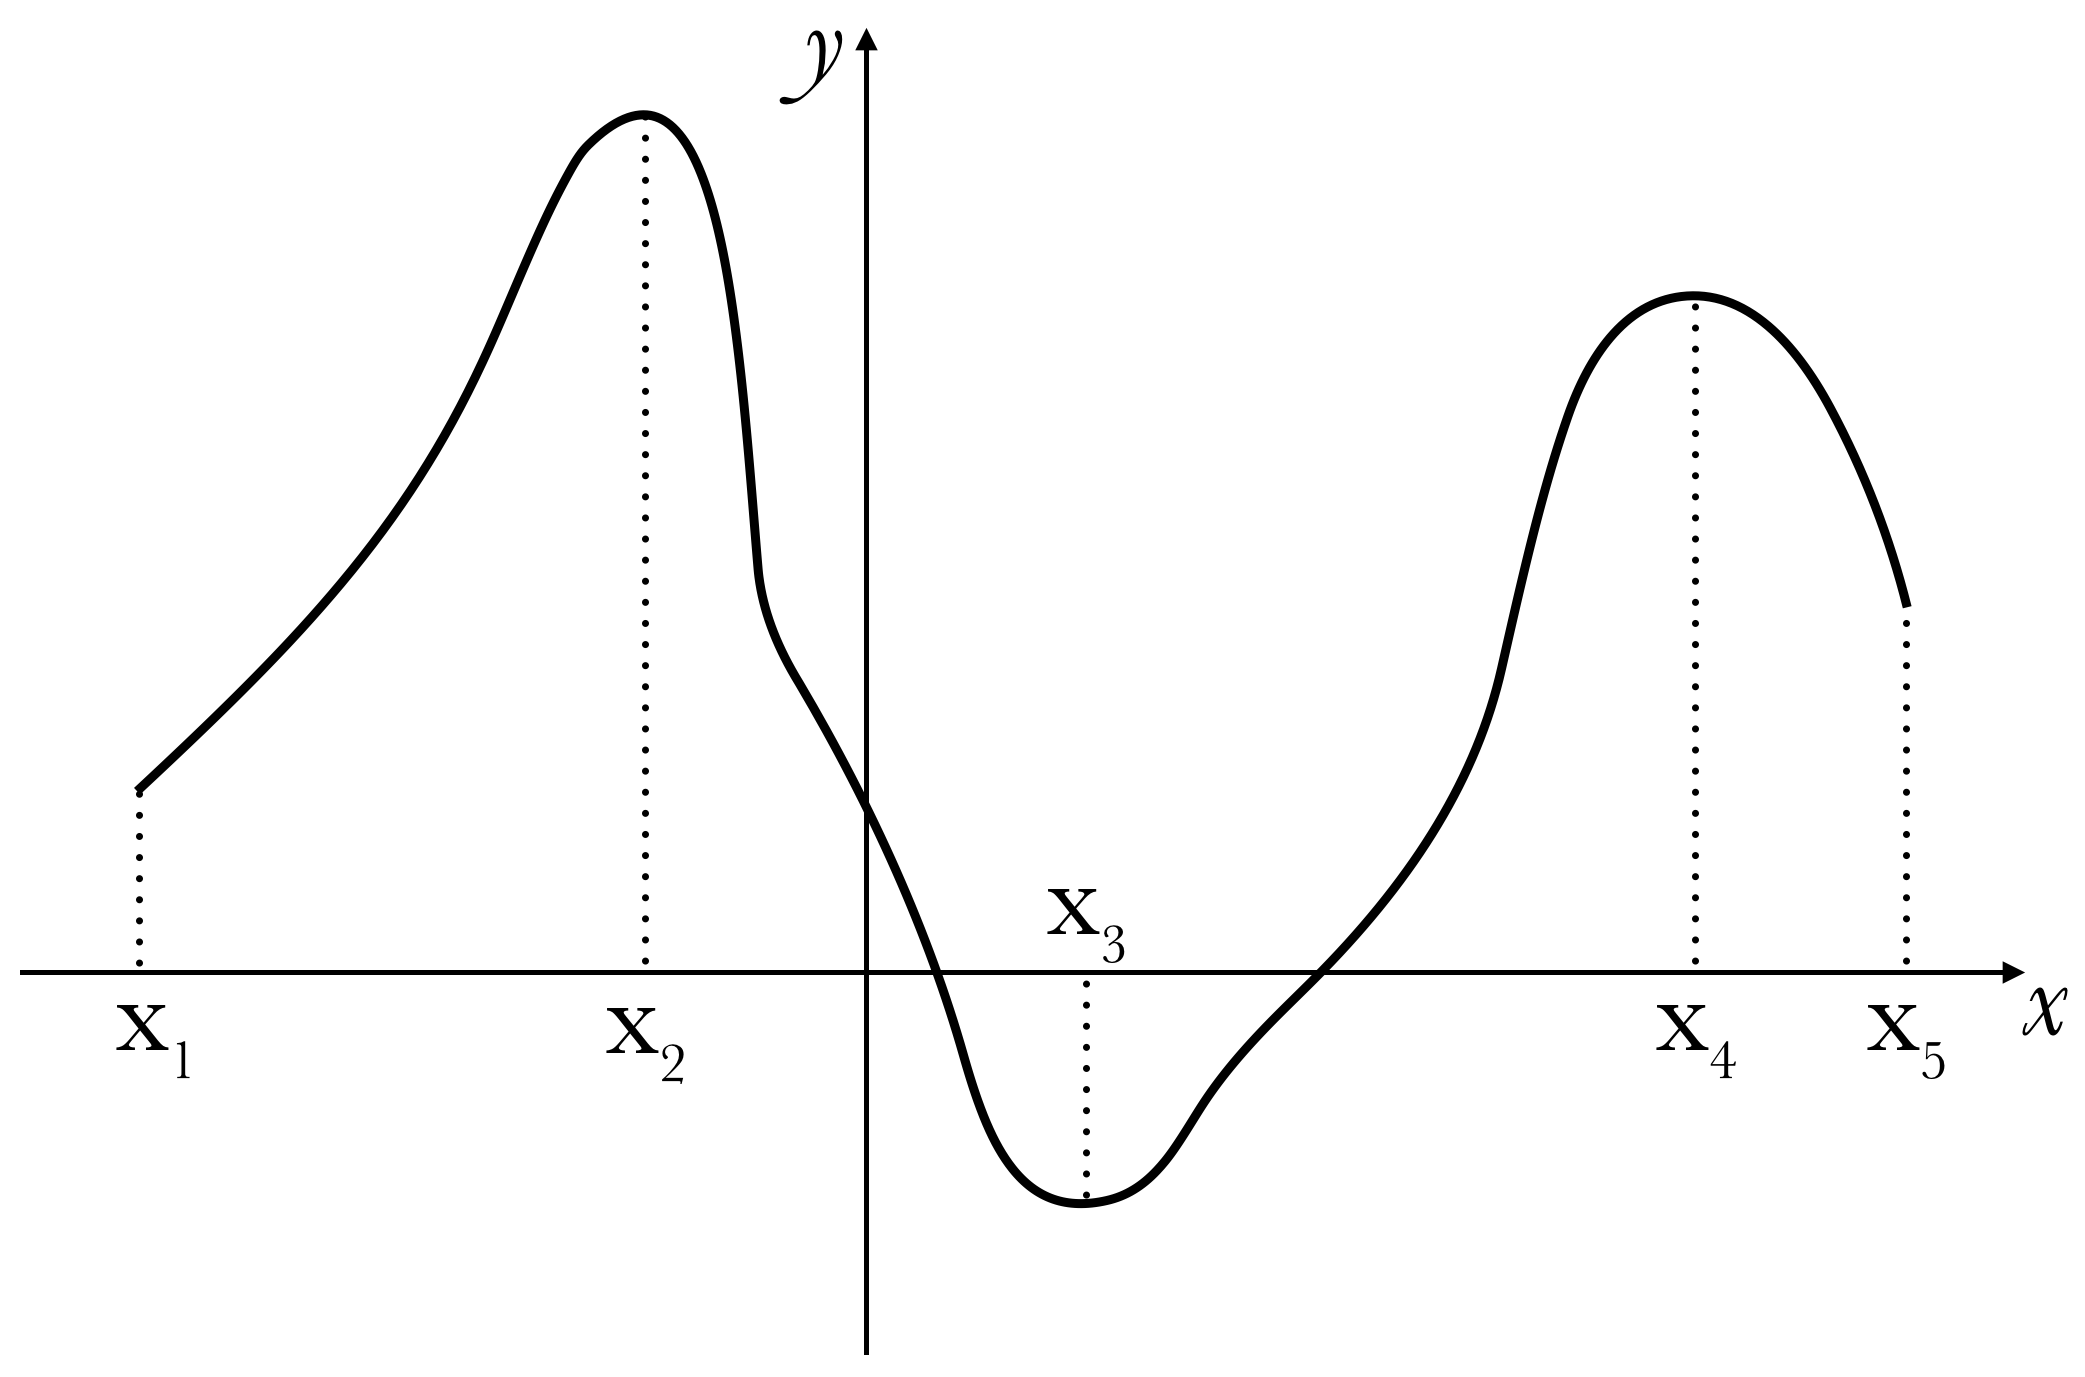
\includegraphics[width=0.4\textwidth]{img/funz_8.png}
  %\caption{}
  %\label{fig:1_2}
\end{figure}
\end{esempio}
\subsection{Parità}
%label{}
La caratteristica della parità va a verificare se il grafico della funzione 
che stiamo studiando è simmetrico rispetto all'asse delle $Y$, cioè il 
grafico è speculare rispetto all'asse, o se il grafico della funzione è 
simmetrico rispetto all'origine. Nel primo caso parleremo di \textsc{parità} 
della funzione, nel secondo caso parleremo di \textsc{disparità} della 
funzione.\\

Ovviamente non tutte le funzioni presenteranno questa simmetria, possiamo 
però individuare delle condizioni che, se presenti nella funzione, ci 
assicurano che questa è pari o dispari.\\

\begin{definizione}
Sia data una funzione $y=f(x)$, avente dominio $D$ tale che per ogni $x\in D$ 
anche $-x\in D$. Una funzione si dice \textsc{pari} in $D$ se \\
$$f(-x)=f(x)$$
per ogni $x\in D$.
\end{definizione}

\begin{figure}[htpb!]
  \centering
  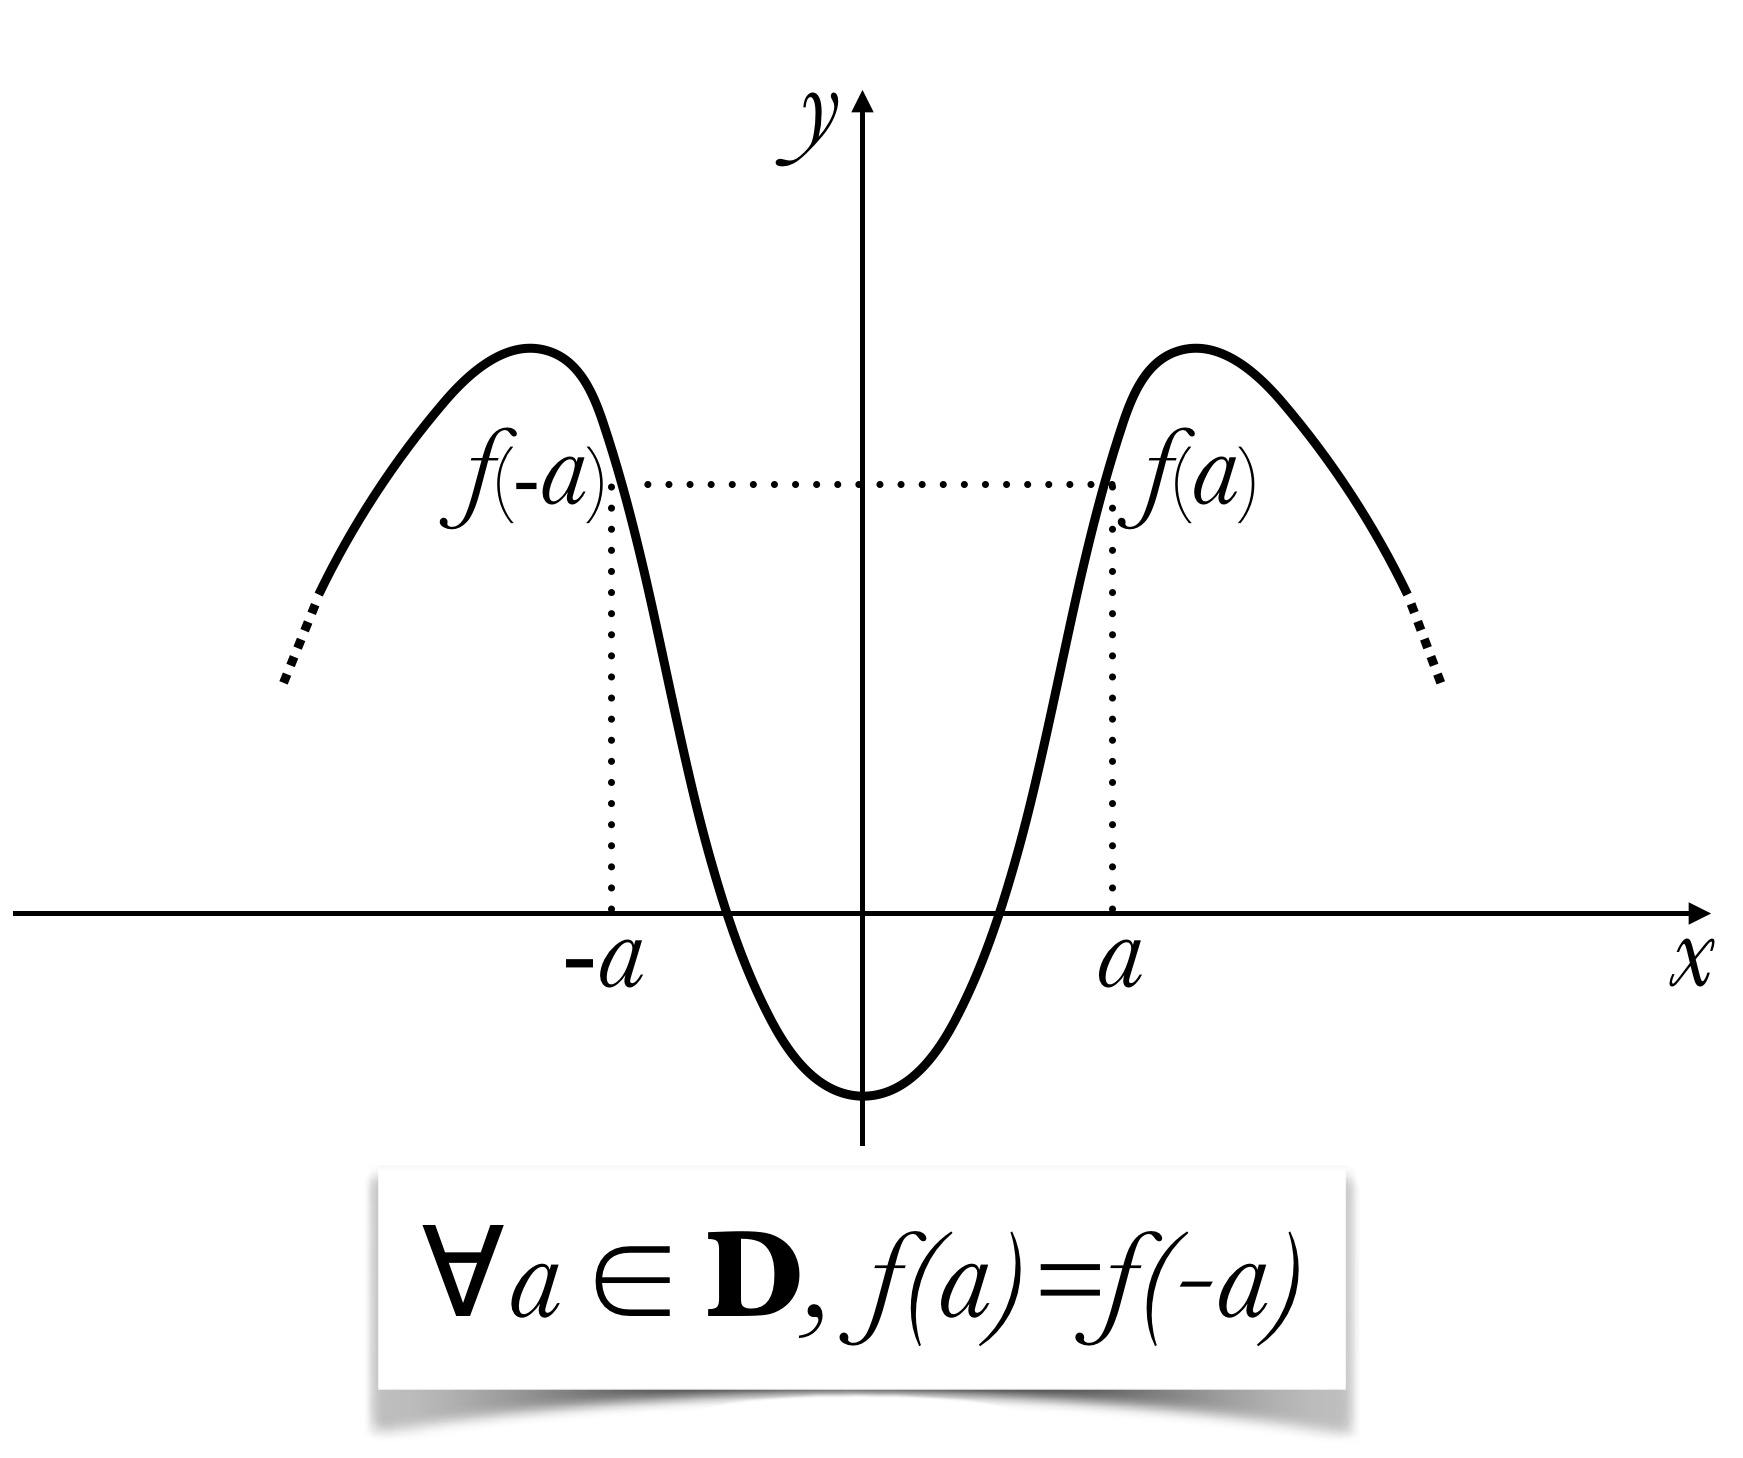
\includegraphics[width=0.5\textwidth]{img/funz_9.png}
  %\caption{}
  %\label{fig:1_2}
\end{figure}
%

Se una funzione è pari, il suo grafico è simmetrico rispetto all'asse $Y$. 
Infatti se $P(x;y)$ appartiene al grafico anche $P'(-x;y)$ vi appartiene. 
Sottolineiamo ancora che la condizione di parità per una funzione è $f(-x)= 
f(x)$.\\   

\begin{esempio} Verificare se una funzione è o non è pari.\\
Per verificare se una funzione è pari basta sostituire nella funzione $-x$ al 
posto di $x$ e verificare se la nuova $f(-x)$ è uguale alla funzione di 
partenza, cioè se $f(-x)=f(x)$. Se prendiamo la funzione 
$$f(x)=\frac{x^2+3}{x+2}$$ \underline{non} è pari, infatti 
$$f(-x)=\frac{(-x)^2+3}{(-x)+2}=\frac{x^2+3}{-x+2}\neq f(x).$$
\end{esempio}

\begin{definizione}
Sia data una funzione $y=f(x)$, avente dominio $D$ tale che per ogni $x\in D$ 
anche$ -x\in D.$ Una funzione si dice \textsc{dispari} in $D$ se\\
$$f(-x)=-f(x)$$
per ogni $x\in D$.
\end{definizione}

\begin{figure}[htpb!]
  \centering
  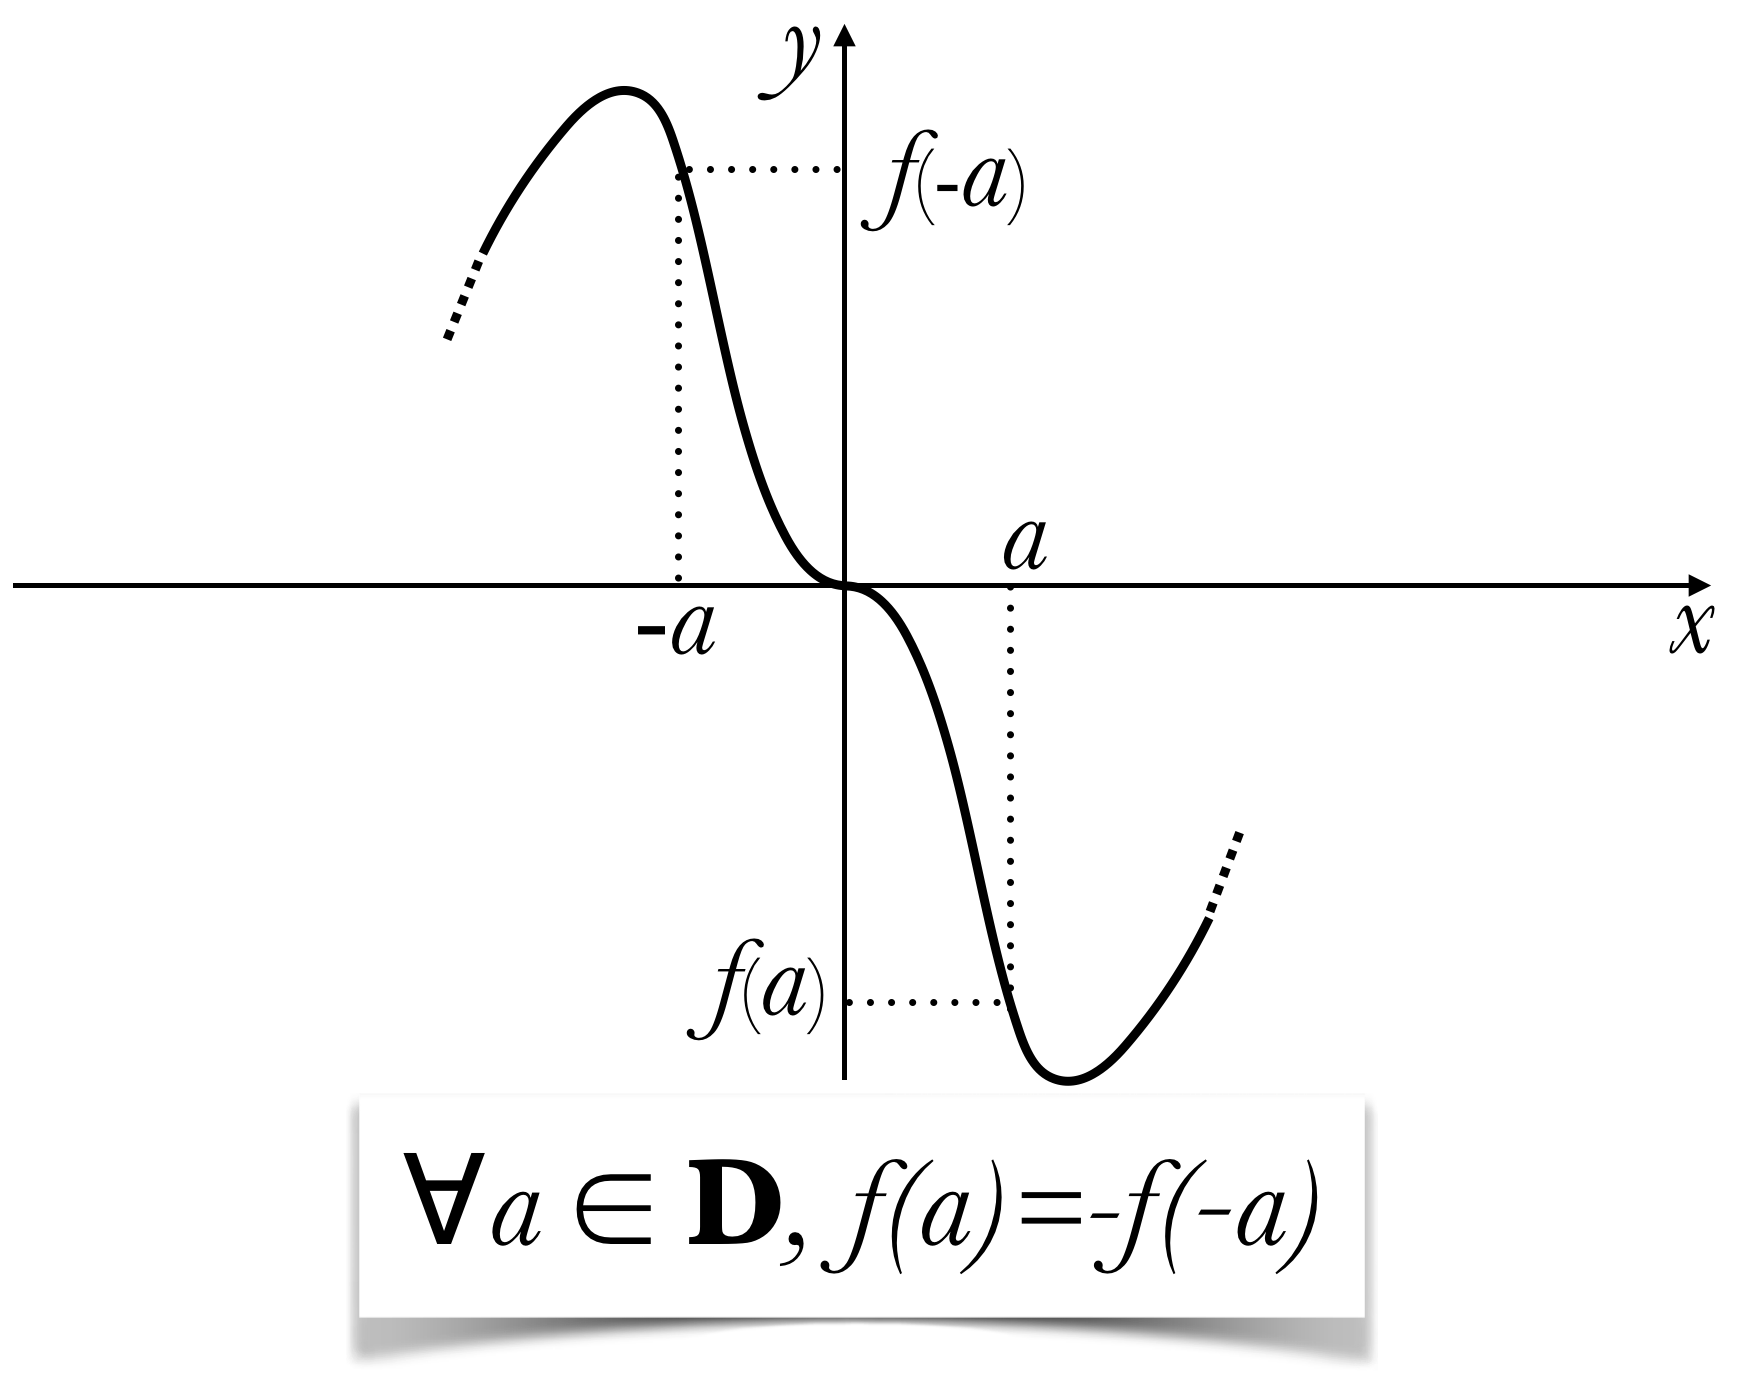
\includegraphics[width=0.5\textwidth]{img/funz_10.png}
  %\caption{}
  %\label{fig:1_2}
\end{figure}
%

Se una funzione è dispari, il suo grafico è simmetrico rispetto all'origine. 
Infatti se $P(x;y)$ appartiene al grafico anche $P'(-x;-y)$ vi appartiene. 
Sottolineiamo ancora che la condizione di disparità per una funzione è 
$f(-x)= -f(x)$. \\

\begin{esempio} Verificare se una funzione è o non è dispari.\\
Per verificare se una funzione è dispari basta sostituire nella funzione $-x$ 
al posto di $x$ e verificare se la nuova $f(-x)$ è uguale alla funzione di 
partenza cambiata di segno, cioè se $f(-x)=-f(x)$. Se prendiamo la funzione 
$$f(x)=\frac{x}{x^2+2}$$ è dispari, infatti 
$$f(-x)=\frac{(-x)}{(-x)^2+2}=\frac{-x}{x^2+2}=-\frac{x}{x^2+2}= -f(x).$$
\end{esempio}

\subsection{Periodicità}
%label{}
La periodicità di una funzione specifica se questa si ripete uguale a sé 
stessa ad intervalli regolari.\\

\begin{definizione}
Una funzione $y=f(x)$, $f(x): A\to \mathbb{R}$ si dice \textsc{periodica} di 
periodo $T>0$ di periodo $T>0$ se$\forall x\in A\rightarrow (x+T)\in A$e 
possiamo scrivere 
 $$f(x+T)=f(x)$$\\
\end{definizione}

\begin{figure}[htpb!]
  \centering
  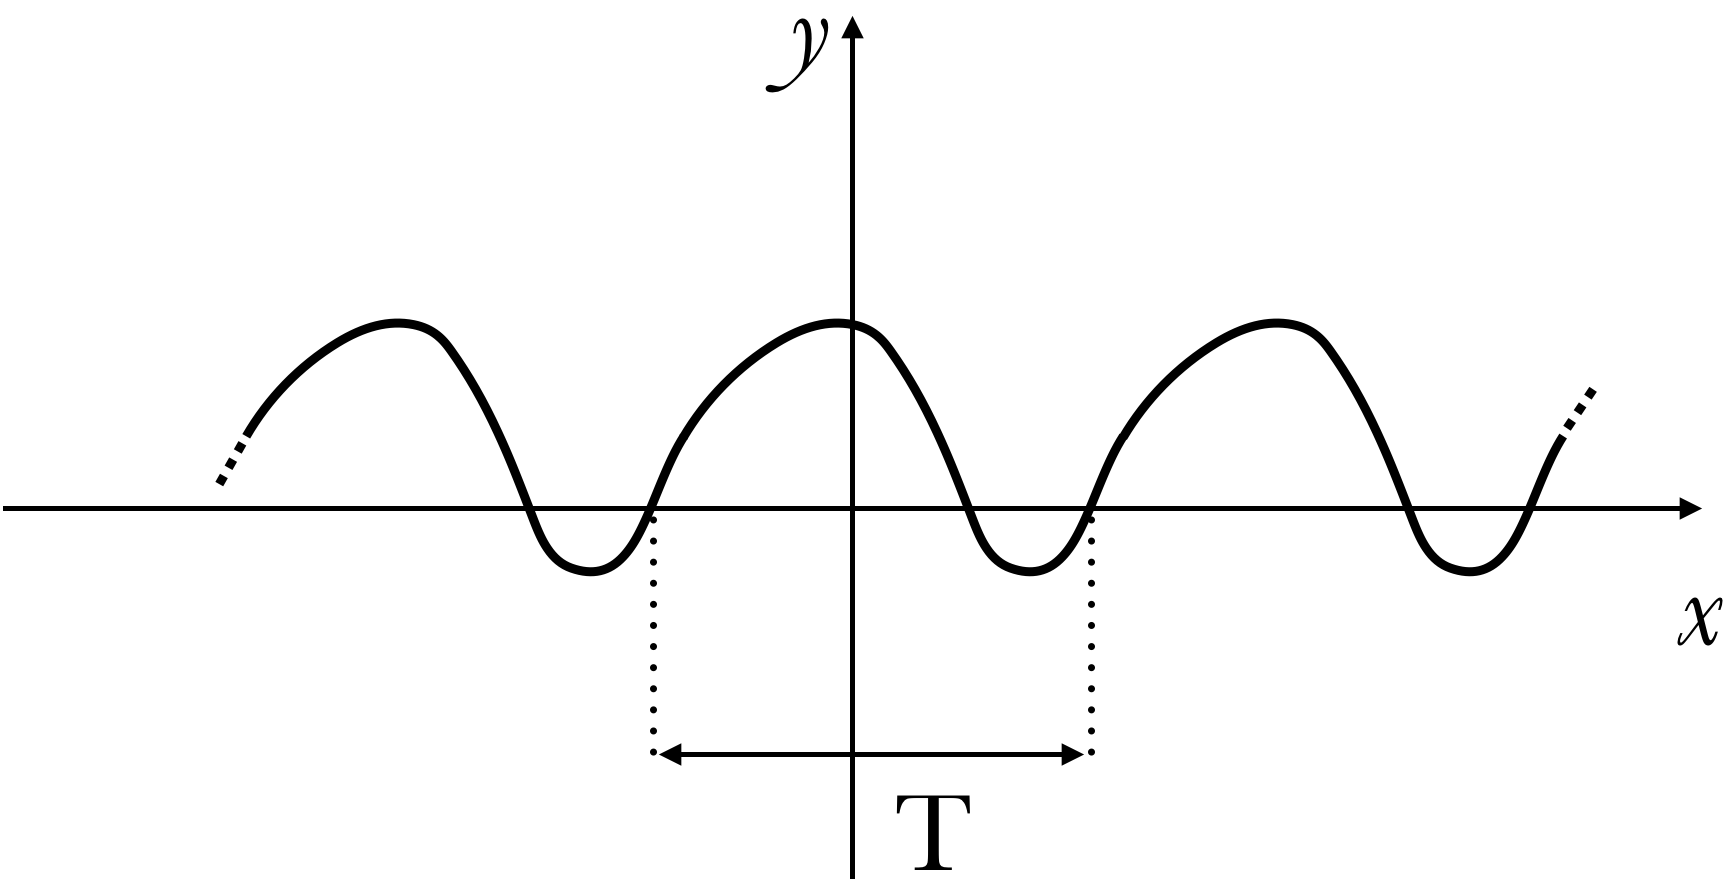
\includegraphics[width=0.45\textwidth]{img/funz_11a.png} \quad 
  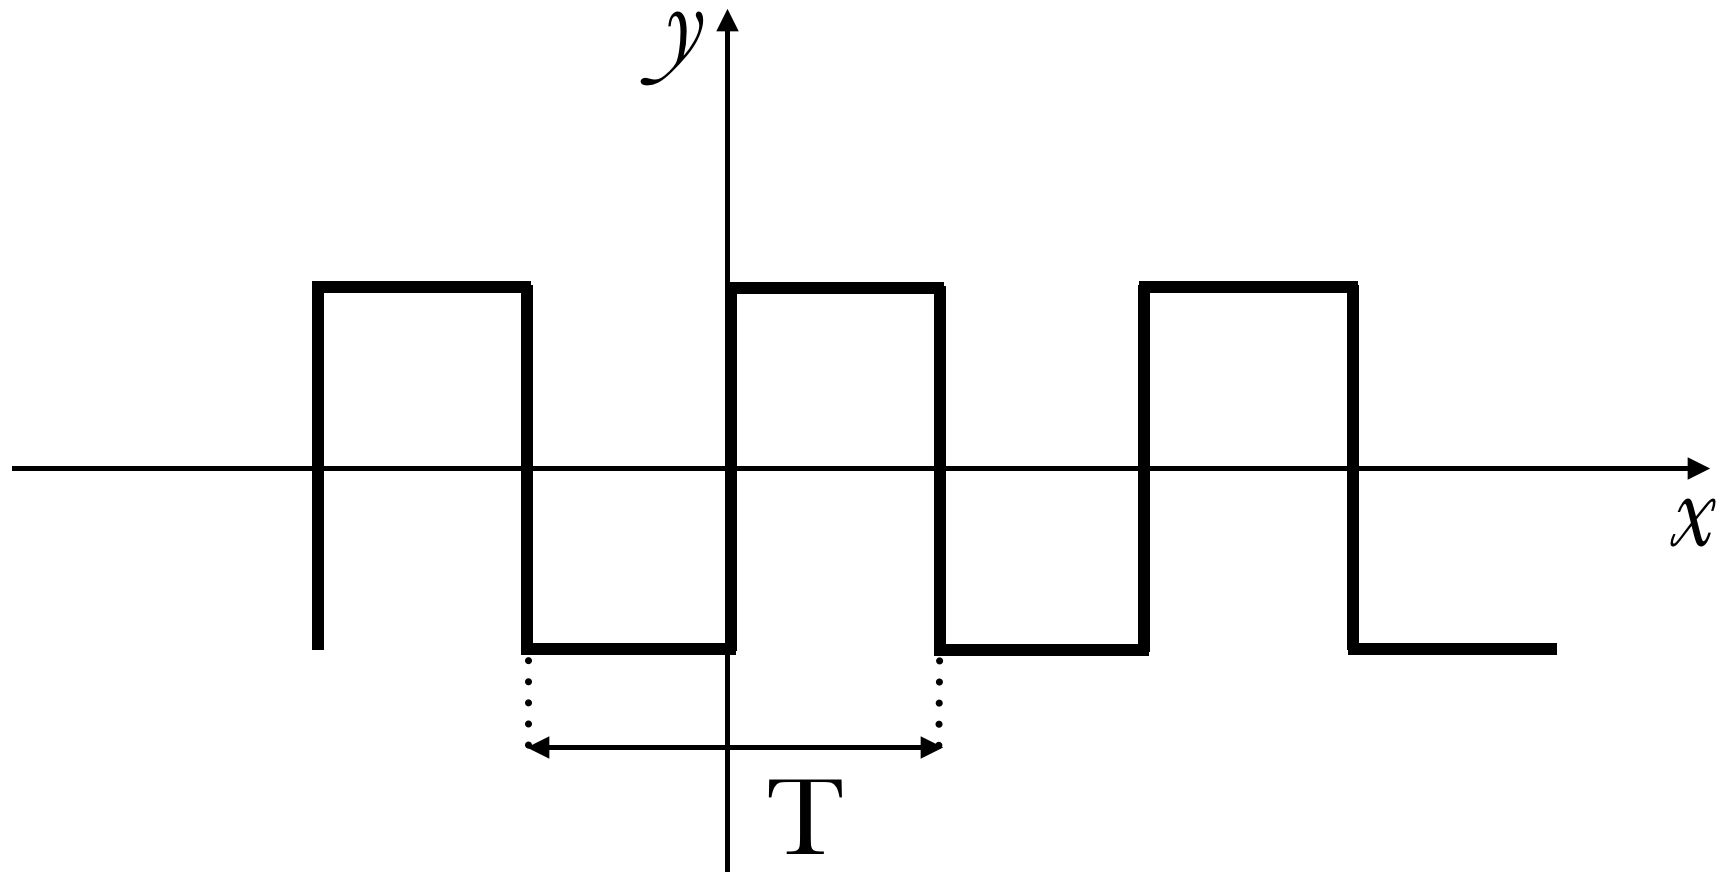
\includegraphics[width=0.45\textwidth]{img/funz_11b.png}
  %\caption{}
  %\label{fig:1_2}
\end{figure}


\begin{esempio} Calcolare il periodo di una funzione.\\
Calcoliamo il periodo della  funzione goniometrica $$y=\sin{7x}$$ con due 
possibili procedure:
\begin{itemize}
  \item[\textsf{Procedura a)}] La funzione ha per definizione periodo 
$T$ se, con $k$ intero,
$$\sin[(7(x+kT)]=\sin4x$$
cioè,
$$\sin[(7x+7kT)]=\sin4x$$
poichè la funzione seno ha periodo $2\pi$, allora
$$\sin[7x+7kT]=\sin[7x+2k\pi]$$
e l'uguaglianza è quindi valida se $7T=2\pi$ da cui
$$T=\frac{2\pi}{7}.$$

  \item[\textsf{Procedura b)}] La funzione $y'=\sin7x'$ viene dalla 
trasformazione della funzione $y=\sin x$, che ha periodo $T=2\pi$, mediante 
una sostituzione $7x'=x$, ovvero $x'=\frac{x}{7}$. Se l'asse delle ascisse 
viene così contratto di un fattore $\frac{x}{7}$, il periodo $T'$ subirà la 
stessa contrazione e pertanto è pari a $$T'=\frac{x}{7}(2\pi)=\frac{2\pi}{7}$$
\end{itemize}
\end{esempio}

Se due funzioni $f(x)$ e $g(x)$ hanno periodi diversi $T_f$ e $T_g$, 
rispettivamente, le funzioni $f(x)\pm g(x)$, $f(x)\cdot g(x)$ e 
$\frac{f(x)}{g(x)}$ hanno un periodo pari al m.c.m. tra $T_f$ e $T_g$ 
nell'ipotesi che $\frac{T_f}{T_g}$ sia un numero razionale e diverso da 1. Se 
il rapporto è irrazionale le precedenti combinazioni di funzioni non sono 
periodiche. Se $T_f=T_g$ il periodo globale è minore o uguale del periodo 
comune.\\

\begin{esempio} Calcolare il periodo di combinazioni di funzioni periodiche e 
non periodiche.\\
  \begin{itemize}
  \item[a)] $f(x)=\sin x+\cos 3x$ è periodica di $2\pi$ che è 
il m.c.m. tra $T_f=2\pi$ e $T_g=\frac{2}{3}\pi$.
  
  \item[b)] $f(x)=\sin x+\cos \pi x$ non è periodica perché il 
rapporto $\frac{T_f}{T_g}\notin \mathbb{Q}$, infatti $T_f=2\pi$ e $T_g=2$, 
per cui $\frac{2\pi}{2}=\pi\notin\mathbb{Q}$
  
  \item[c)] $f(x)=\sin \frac{x}{2}-\cos 3x+\tan x$ dove 
$T_{\sin \frac{x}{2}}=4\pi$, $T_{\cos 3x}=\frac{2}{3}\pi$, $T_{\tan}=\pi$
  
  \item[d)] Se consideriamo la funzione 
$$f(x)=\frac{1}{\log[\sin x]}$$ il periodo è $2\pi$
\end{itemize}
\end{esempio}

Se una funzione è periodica i valori delle sue ordinate si ripetono con 
regolarità, quindi per studiarne l'andamento su tutto l'asse reale, basterà 
studiarne l'andamento in un singolo periodo. Ripetiamo ancora che la 
condizione di parità per una funzione è $f(x+T)=f(x)$ con $T$ periodo.
%
%
\subsection{Limitatezza}
%label{}
La limitatezza di una funzione valuta se le ordinate di una funzione 
raggiungono un valore massimo e un valore minimo, oppure non hanno un 
limite.\\


\begin{definizione}
Consideriamo una funzione $f: A\to \mathbb{R}$, la funzione si dice:
  \begin{itemize}
  \item[$\rhd$]\textsc{limitata superiormente} se il suo 
codominio $f(A)$ ha un limite superiore $k$:
$$\exists k\in \mathbb{R} \vert \forall x\in A,\, k\geq f(x)$$ 
  \item[$\rhd$]\textsc{limitata inferiormente} se il suo 
codominio f(A) ha un limite inferiore $k$: 
$$\exists k\in \mathbb{R} \vert \forall x\in A,\, k\leq f(x)$$

  \item[$\rhd$]\textsc{limitata} se il suo codominio $f(A)$ è 
limitato sia superiormente che inferiormente:
$$\exists k\in \mathbb{R},k>0\vert\forall x\in A, \vert f(x)\vert \leq k$$
\end{itemize}

Se una funzione non è limitata da un valore del codominio $k$ si dirà 
illimitata, in particolare:
  \begin{itemize} 
  \item[$\rhd$] \textsc{Illimitata superiormente} se il suo 
codominio $f(A)$ \underline{non} è limitato superiormente;
  \item[$\rhd$] \textsc{Illimitata inferiormente} se il suo 
codominio $f(A)$ \underline{non} è limitato inferiormente;
  \item[$\rhd$] \textsc{Illimitata} se il suo codominio $f(A)$ 
\underline{non} è limitato superiormente \underline{né} inferiormente.
  \end{itemize}
\end{definizione}
%
\begin{esempio} Determinare la limitatezza o illimitatezza di funzioni.\\
In (a) La funzione $f(x)=\log(x)$ è illimitata: né superioremente né 
inferiormente limitata; in (b) La funzione è limitata inferiormente e 
illimitata superiormente; in (c) La funzione $f(x)=\sin{x}$ è limitata sia 
superiormente che inferiormente; in (d) La funzione $f(x)=x^2$ è limitata 
inferiormente e illimitata superiormente.
\begin{figure}[h]
  \centering
  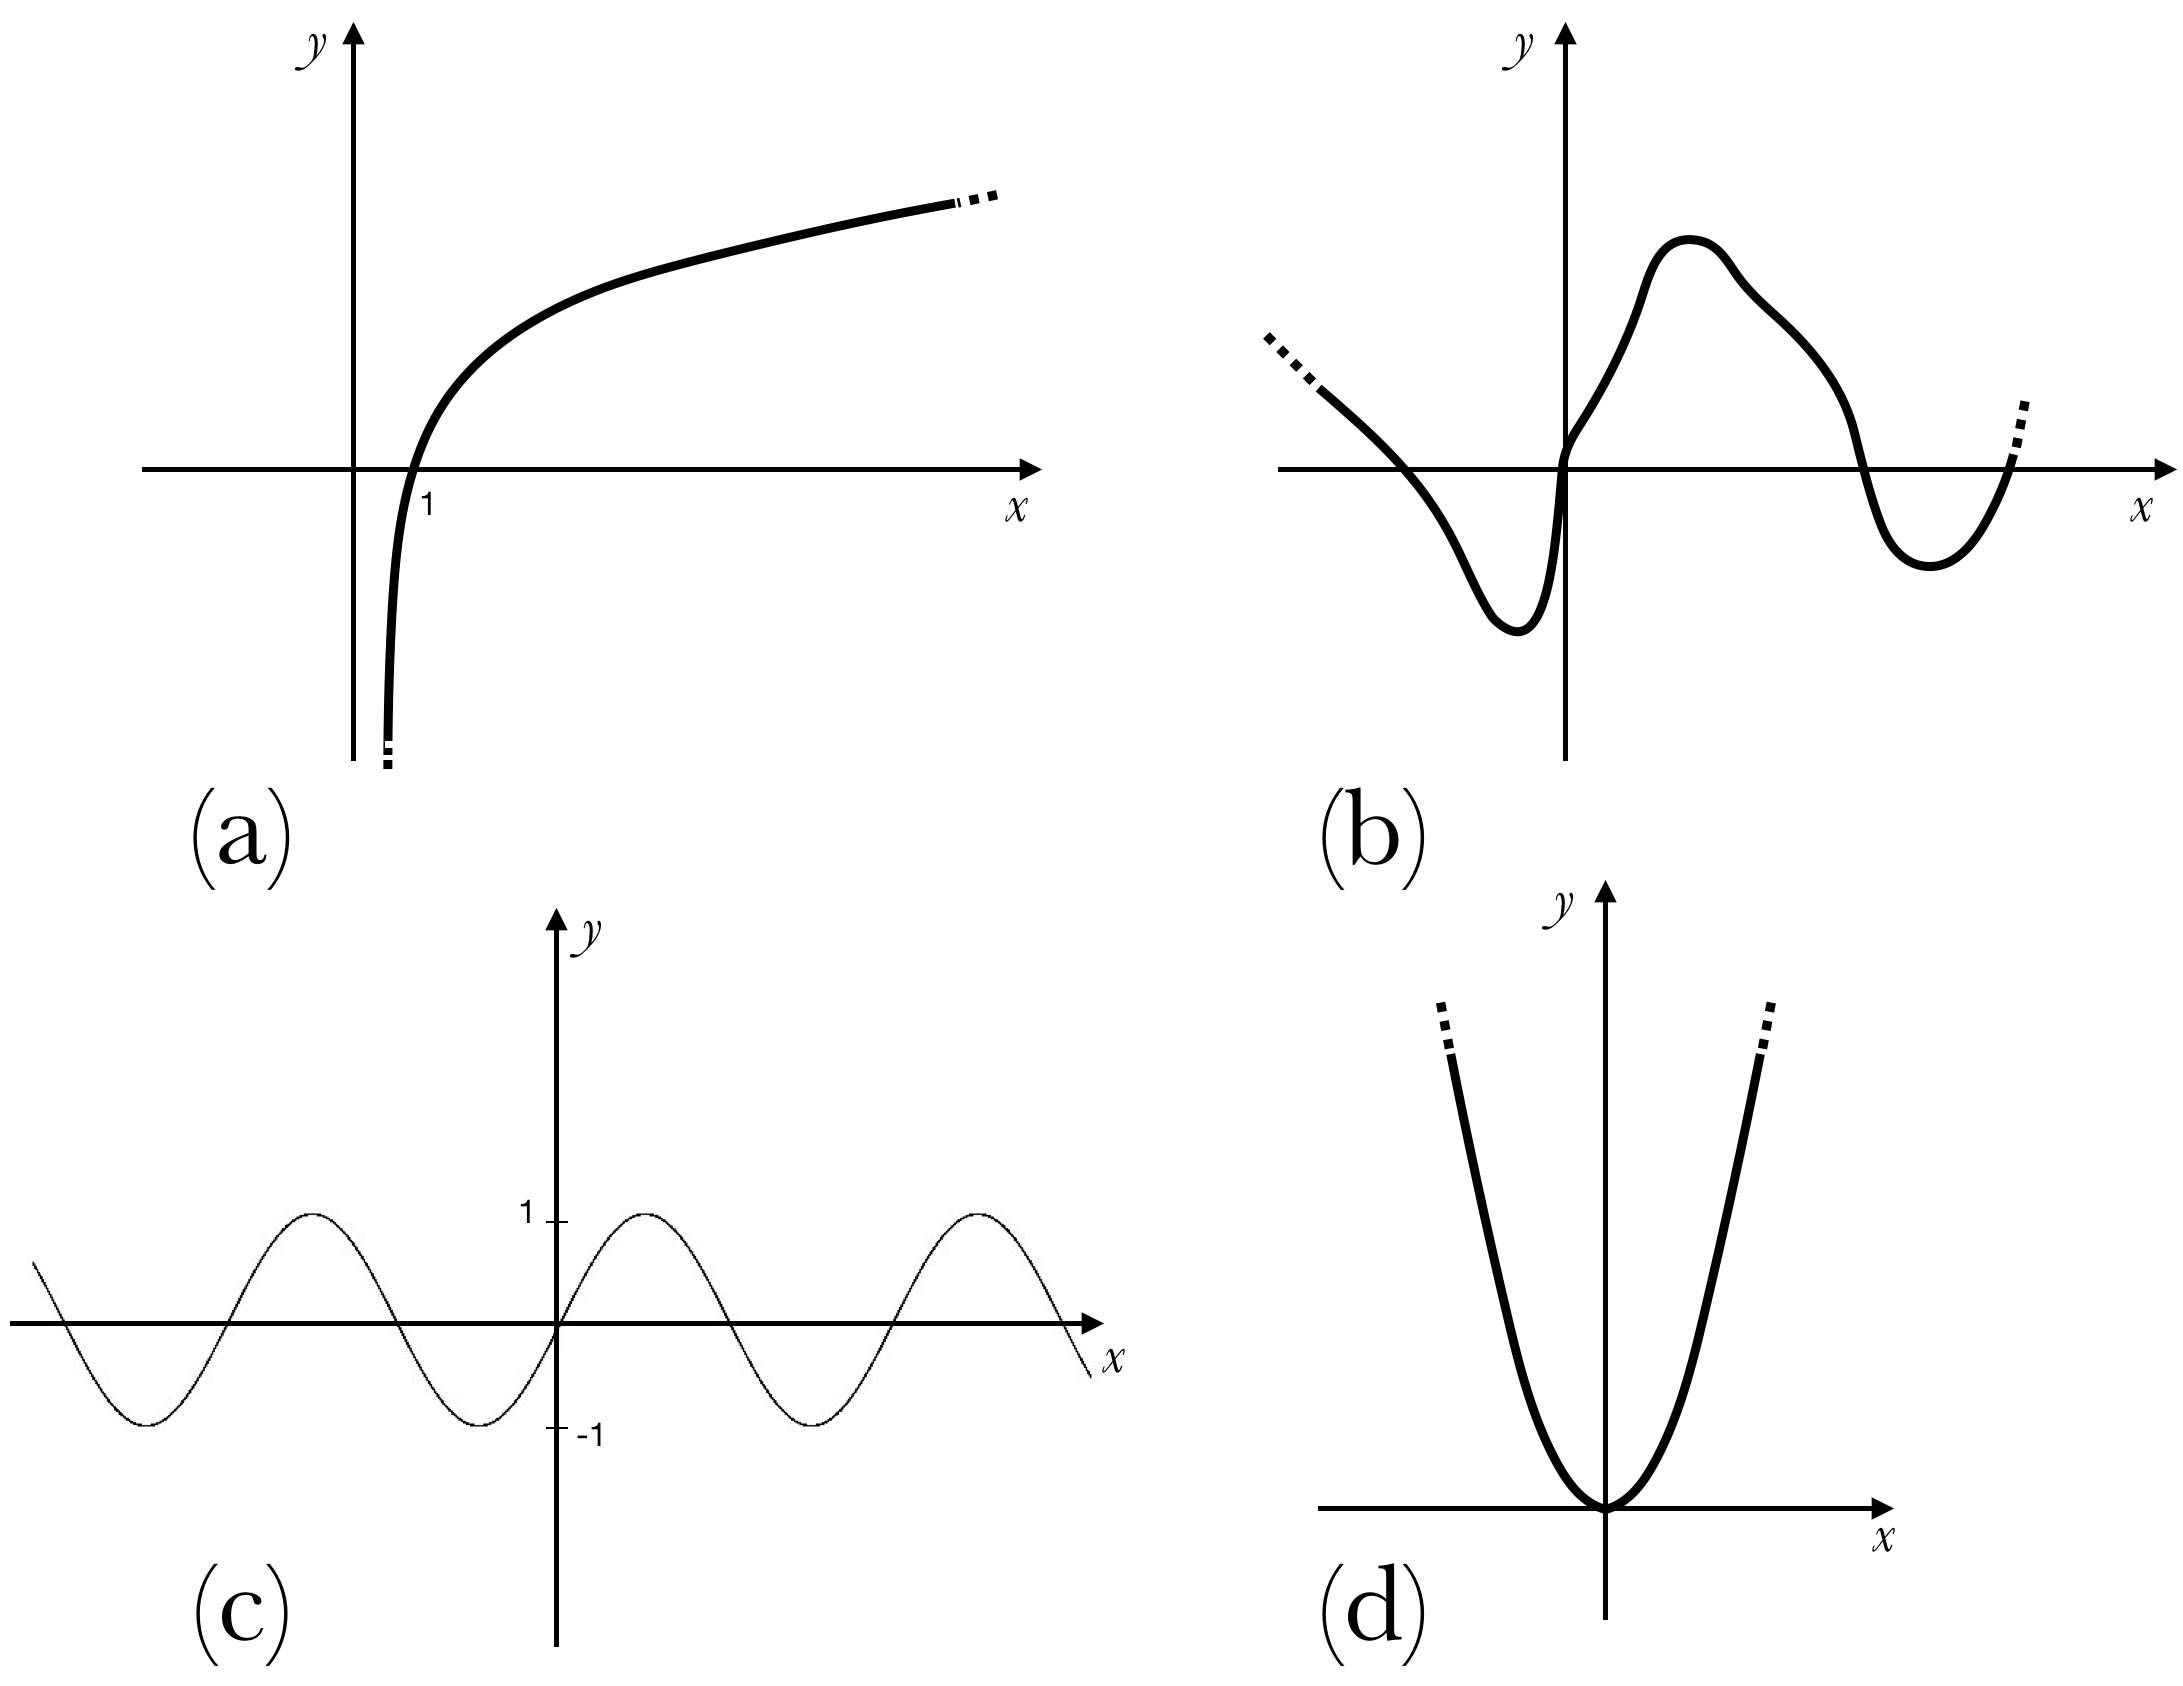
\includegraphics[width=0.85\textwidth]{img/funz_12a.png}
  %\label{fig:1_2}
\end{figure}
\end{esempio}
\newpage
\section{La classificazione delle funzioni}
%label{}
Classifichiamo le possibili funzioni che incontreremo o abbiamo incontrato in 
base alle operazioni che compaiono nella loro espressione analitica. Se 
nell'espressione analitica di una funzione compaiono le operazioni di 
addizione, sottrazione, moltiplicazione, divisione, elevamento a potenza con 
esponente razionale o estrazione di radice siamo di fronte ad una 
\textsc{funzione algebrica}.\\

Le funzioni che non possono essere rappresentate usando solamente le 
operazioni precedentemente ricordate si dicono \textsc{trascendenti}. Tra le 
più note funzioni trascendenti ricordiamo le funzioni goniometriche, quelle 
esponenziali e quelle logaritmiche.\\

A seconda che le funzioni algebriche contengano o meno l'operazione di radice 
e l'operazione di divisione suddividiamo le funzioni algebriche in 
\textsc{razionali fratte}, \textsc{razionali intere} o polinomiali, 
\textsc{irrazionali fratte} e \textsc{irrazionali intere}. \\

\textsf{MEMO!!} Per non creare equivoci ricordiamo che una funzione è 
definita fratta quando il denominatore contiene la variabile indipendente 
$x$, è invece definita irrazionale quando tale variabile appare sotto il 
segno di radice.\\

% TODO non compila!!!!!!!!!!!!!!!!!!!!!!!!!!!!!!!!!!!!!!!!!!!!!!!!!!!
% \Tree [.FUNZIONI [.\textbf{algebriche}  [.razionali fratte intere 
% !{\qbalance} ] [.irrazionali fratte intere !{\qbalance} ] ] 
% [.\textbf{trascendenti} goniometriche esponenziali logaritmiche ] ] \\


\begin{esempio} Classificazione di funzioni.\\
Classifichiamo le seguenti funzioni: 
  \begin{itemize}
  \item[a)] $f(x)=\frac{\sqrt{(x+5)}}{3}$ è una funzione 
irrazionale intera, infatti pur avendo un denominatore, questo non contiene 
la variabile indipendente $x$;
  
  \item[b)] $g(x)=e^{\frac{x}{x-1}}$ è una funzione 
trascendente di tipo esponenziale;

  \item[c)] $h(x)=\sqrt{2}x+4x$ è una funzione razionale 
intera, in quanto la radice compare solo nel numero irrazionale  a 
coefficiente della $\sqrt{2}$ $x$.
  \end{itemize}
\end{esempio}

\section{Funzioni inverse, composte e uguali}
%label{}
Nella rappresentazione insiemistica studiata finora abbiamo sempre visto le 
frecce partire dall'insieme $A$ per arrivare nell'insieme $B$. Esiste una 
possibile lettura al contrario? Se le frecce partissero da $B$, dalle $y$ per 
arrivare alle $x$, ci troveremmo ancora in presenza di una funzione?

\begin{definizione}
Sia $f : A\to B$ una funzione biiettiva. Si dice funzione inversa di $f$ la 
funzione $f^{-1} : B\to A$ che associa a ogni $y$ di $B$ il valore $x$ di $A$ 
tale che $y=f(x)$.
\end{definizione}

\begin{figure}[htpb!]
  \centering
  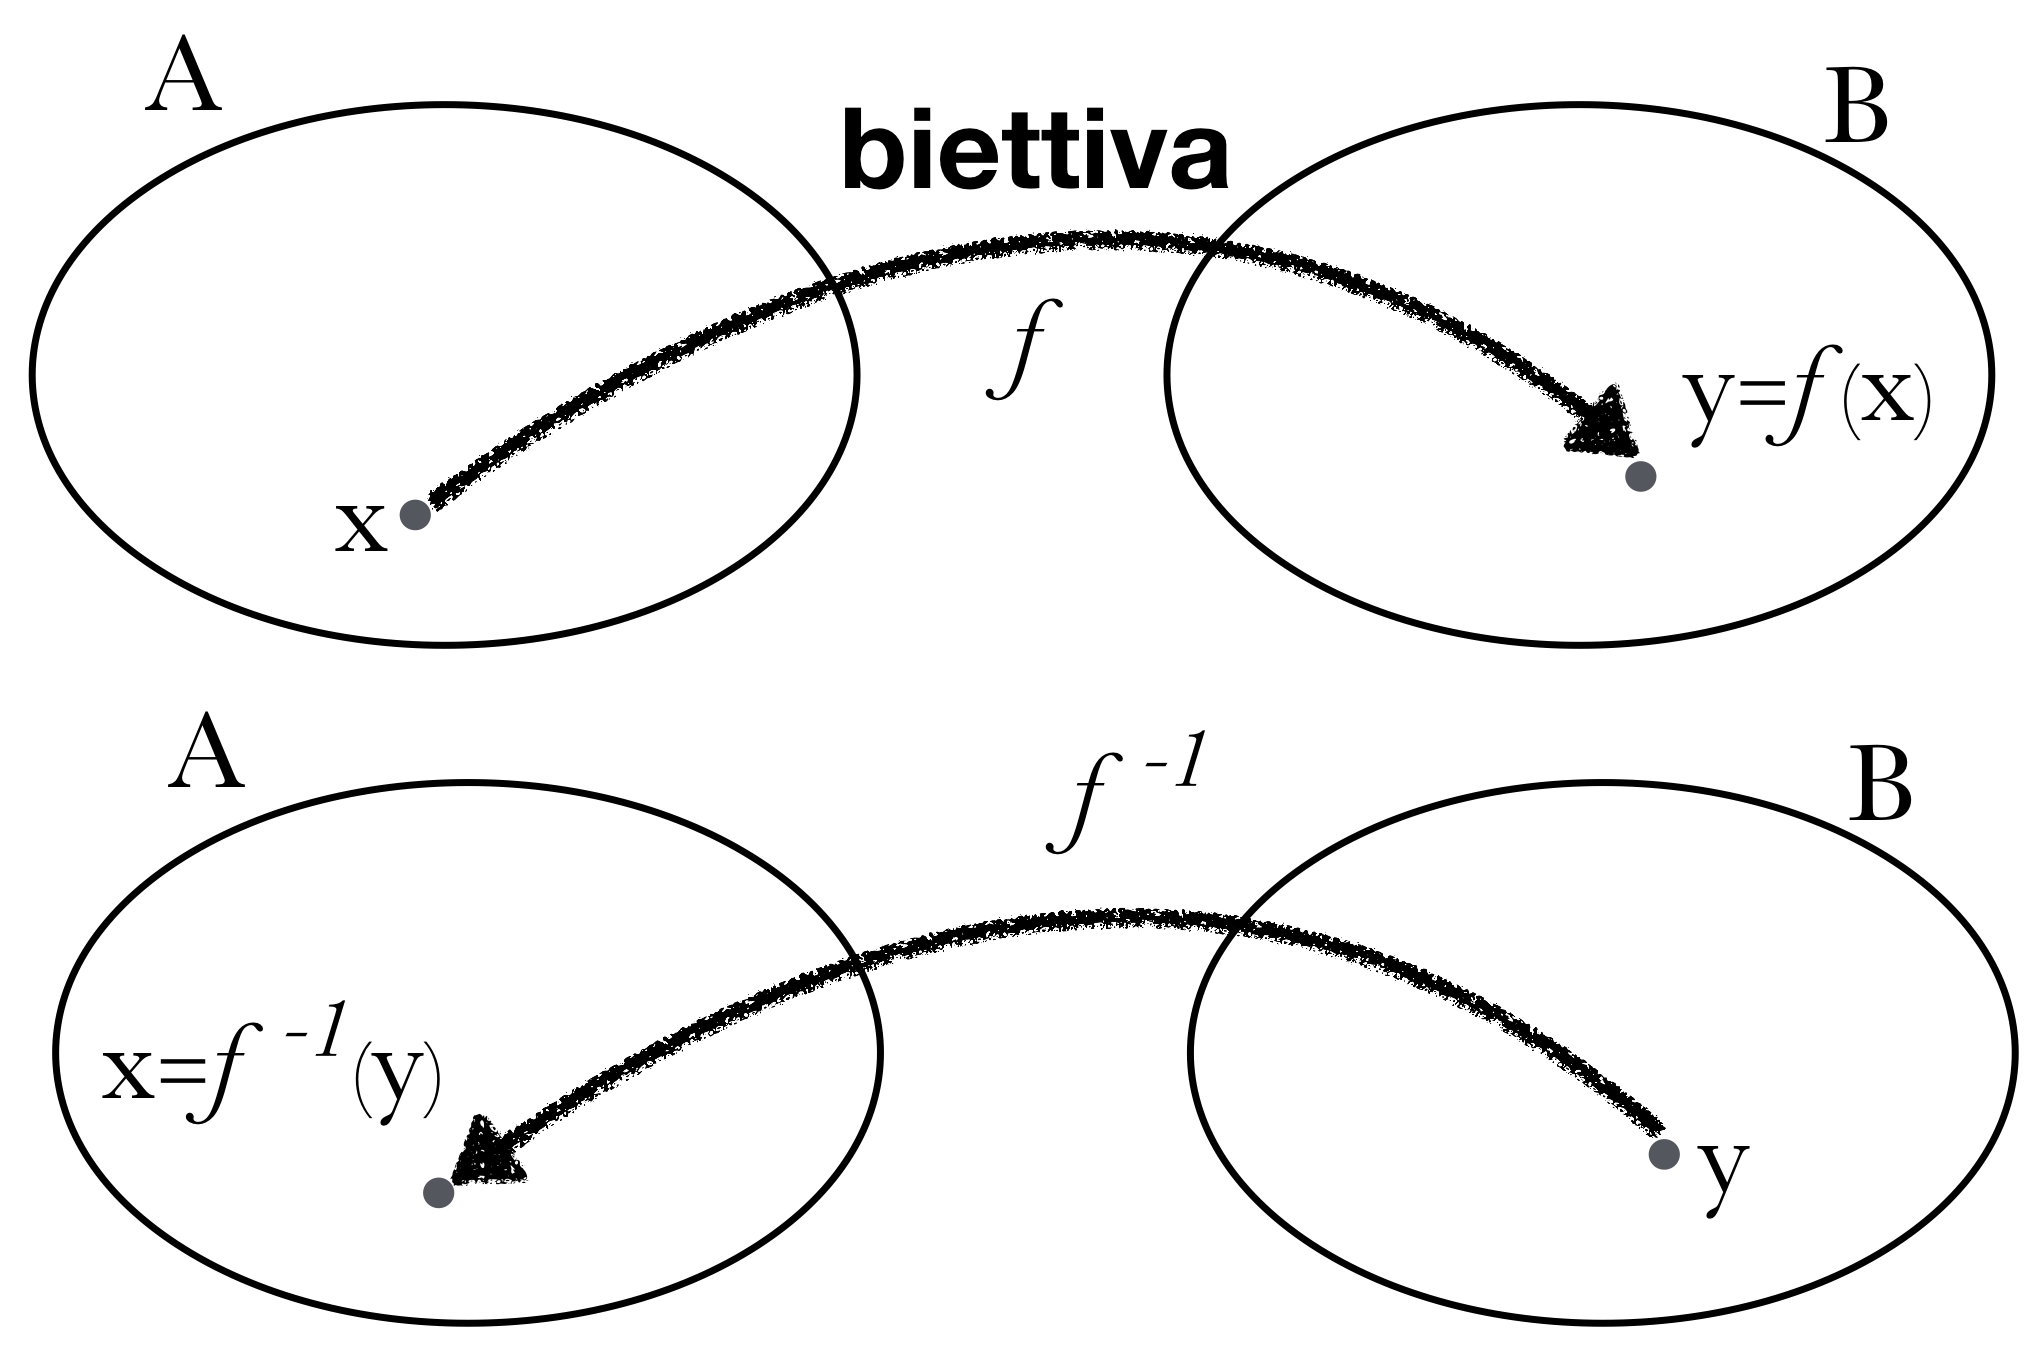
\includegraphics[width=0.45\textwidth]{img/funz_12.png} 
  %\caption{}
  %\label{fig:1_2}
\end{figure}

Notiamo che se una funzione ammette inversa si dice \textsc{invertibile}. 
Significativa è, poi, la relazione tra i codomini e i domini delle due 
funzioni, $f$ e la sua inversa: il dominio di $f^{-1}$ è l'immagine di $f$ e 
l'immagine di $f^{-1}$ è il dominio di $f$.\\

\begin{esempio} Calcolare  e graficare l'inversa di una funzione, verificando 
che sia invertibile.\\ 
Consideriamo la funzione biiettiva $f:\mathbb{R}\to\mathbb{R}$ definita da
$$f(x)=y=3x+2$$
Possiamo ottenere la sua inversa $f^{-1}$ nel seguente modo:
  \begin{itemize}
  \item ricaviamo $x$ in funzione di $y$ dalla relazione 
precedente
$$x=\frac{y-2}{3}$$
  \item sostituiamo la $x$ con $y$ e viceversa.
  \begin{figure}[htpb!]
  \centering
  
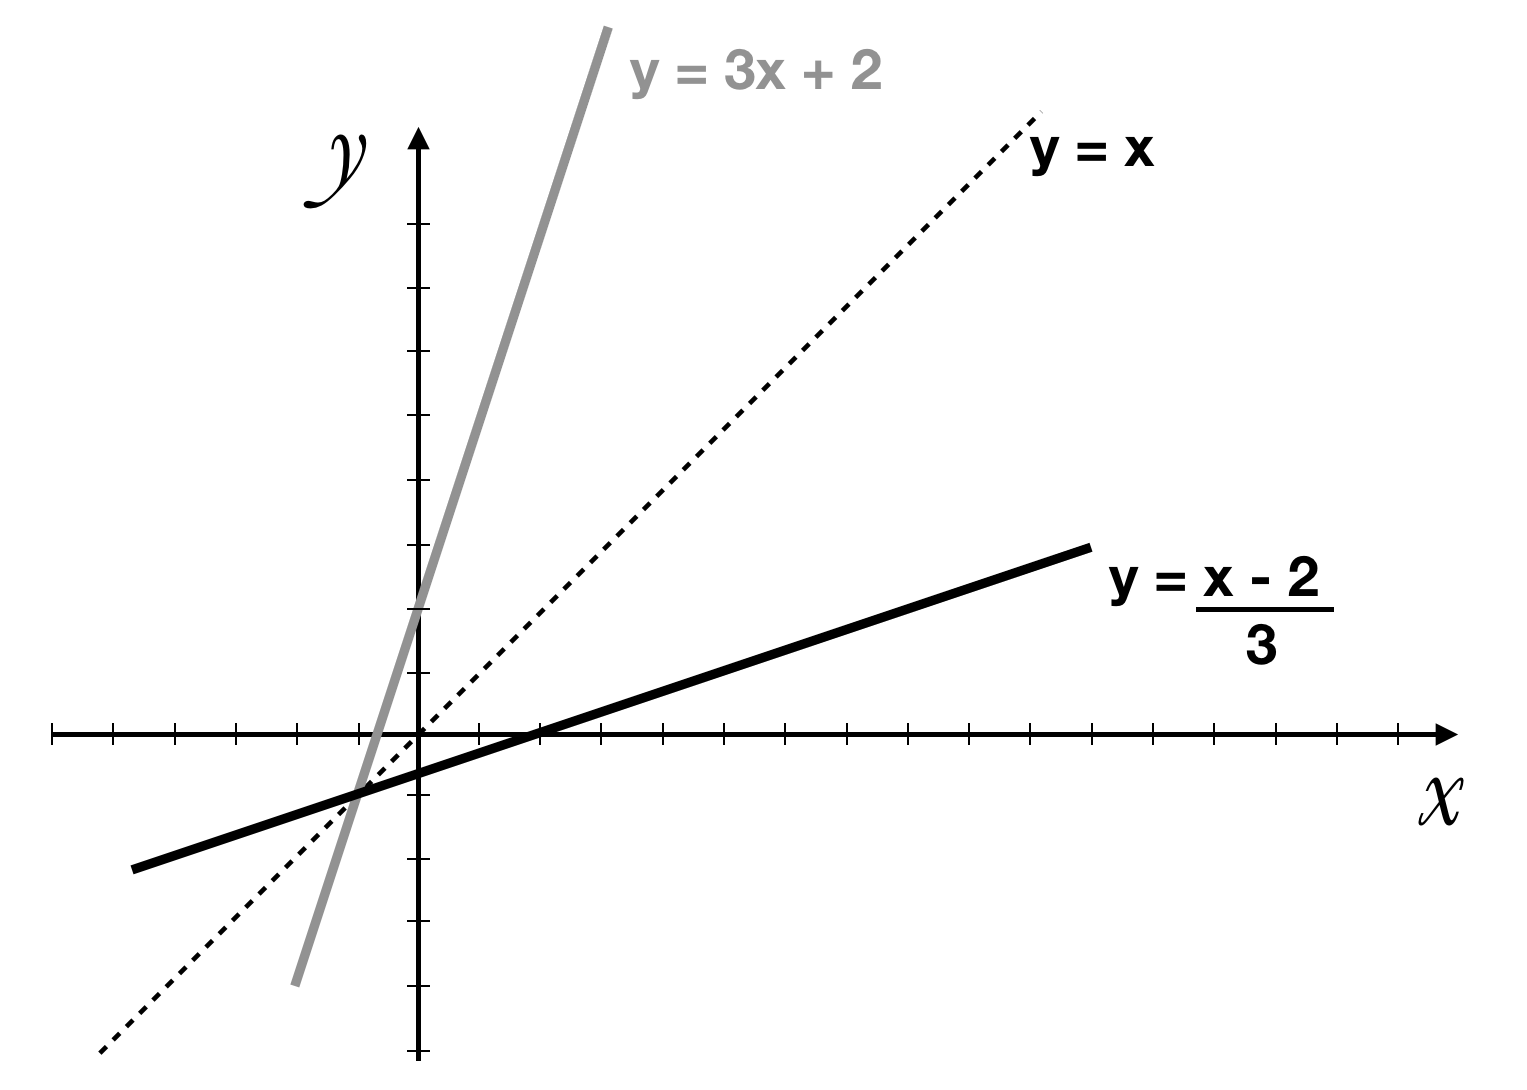
\includegraphics[width=0.5\textwidth]{img/funz_13.png} 
  %\caption{}
  %\label{fig:1_2}
  \end{figure}
  \item notiamo che il grafico della funzione inversa
$$f^{-1}(x)=\frac{x-2}{3}$$
è simmetrico a quello di $f(x)$ rispetto alla bisettrice del primo e terzo 
quadrante, la retta di equazione $y=x$
  \end{itemize}
\end{esempio}

\begin{esempio} Disegnare l'inversa di una funzione che originariamente non 
sia invertibile nel suo dominio. 

La funzione $f:\mathbb{R}\to\mathbb{R}$ tale che $$f(x)=x^2+1$$.
\begin{itemize}
  \item $f$ non ammette funzione inversa perché non è biiettiva, in 
quanto non è iniettiva.
  \begin{figure}[htpb!]
  \centering
  
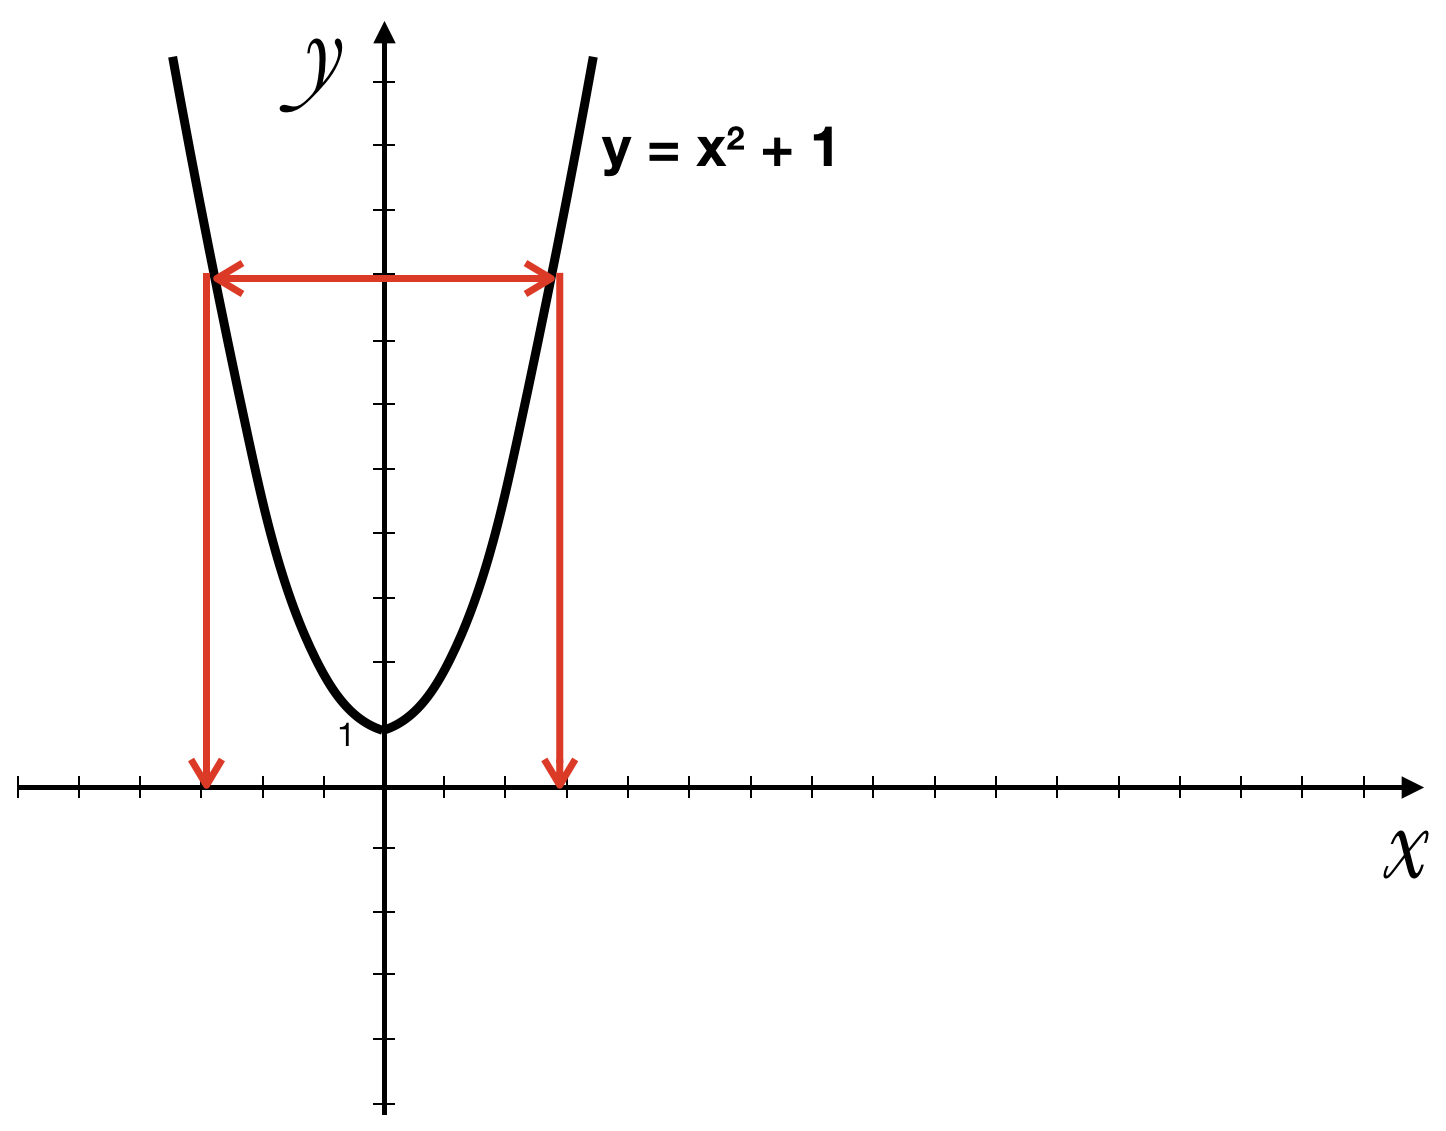
\includegraphics[width=0.45\textwidth]{img/funz_14a.png} %\quad
  
%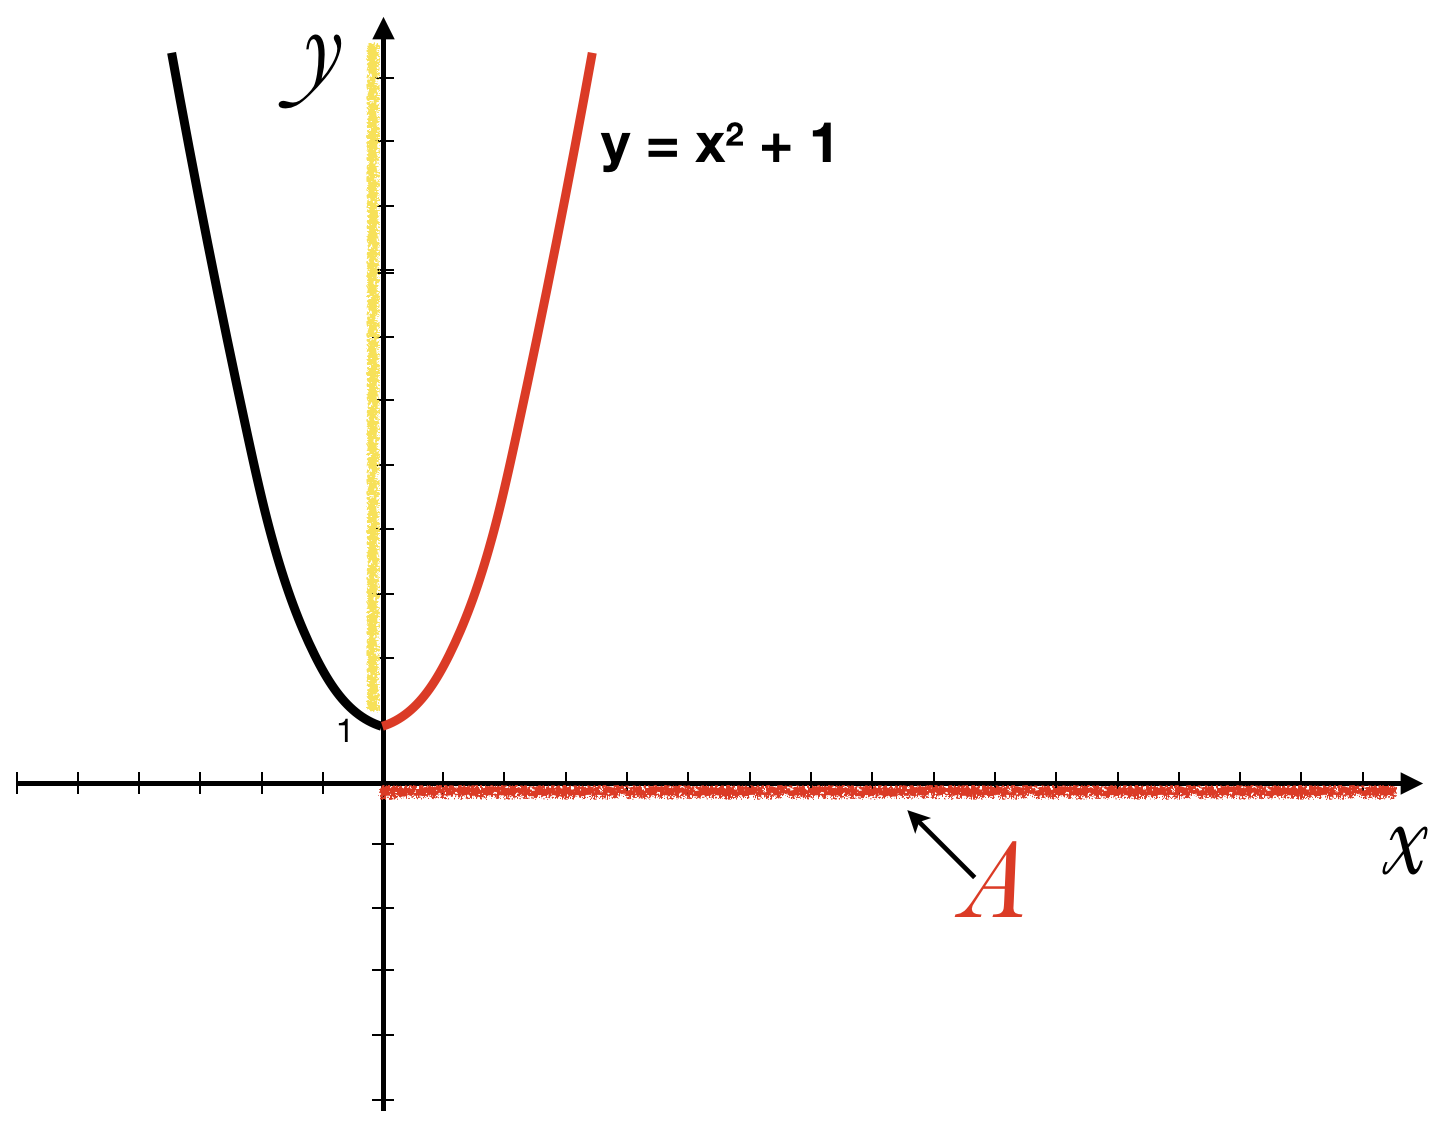
\includegraphics[width=0.7\textwidth]{img/funz_14b.png} \quad
  
%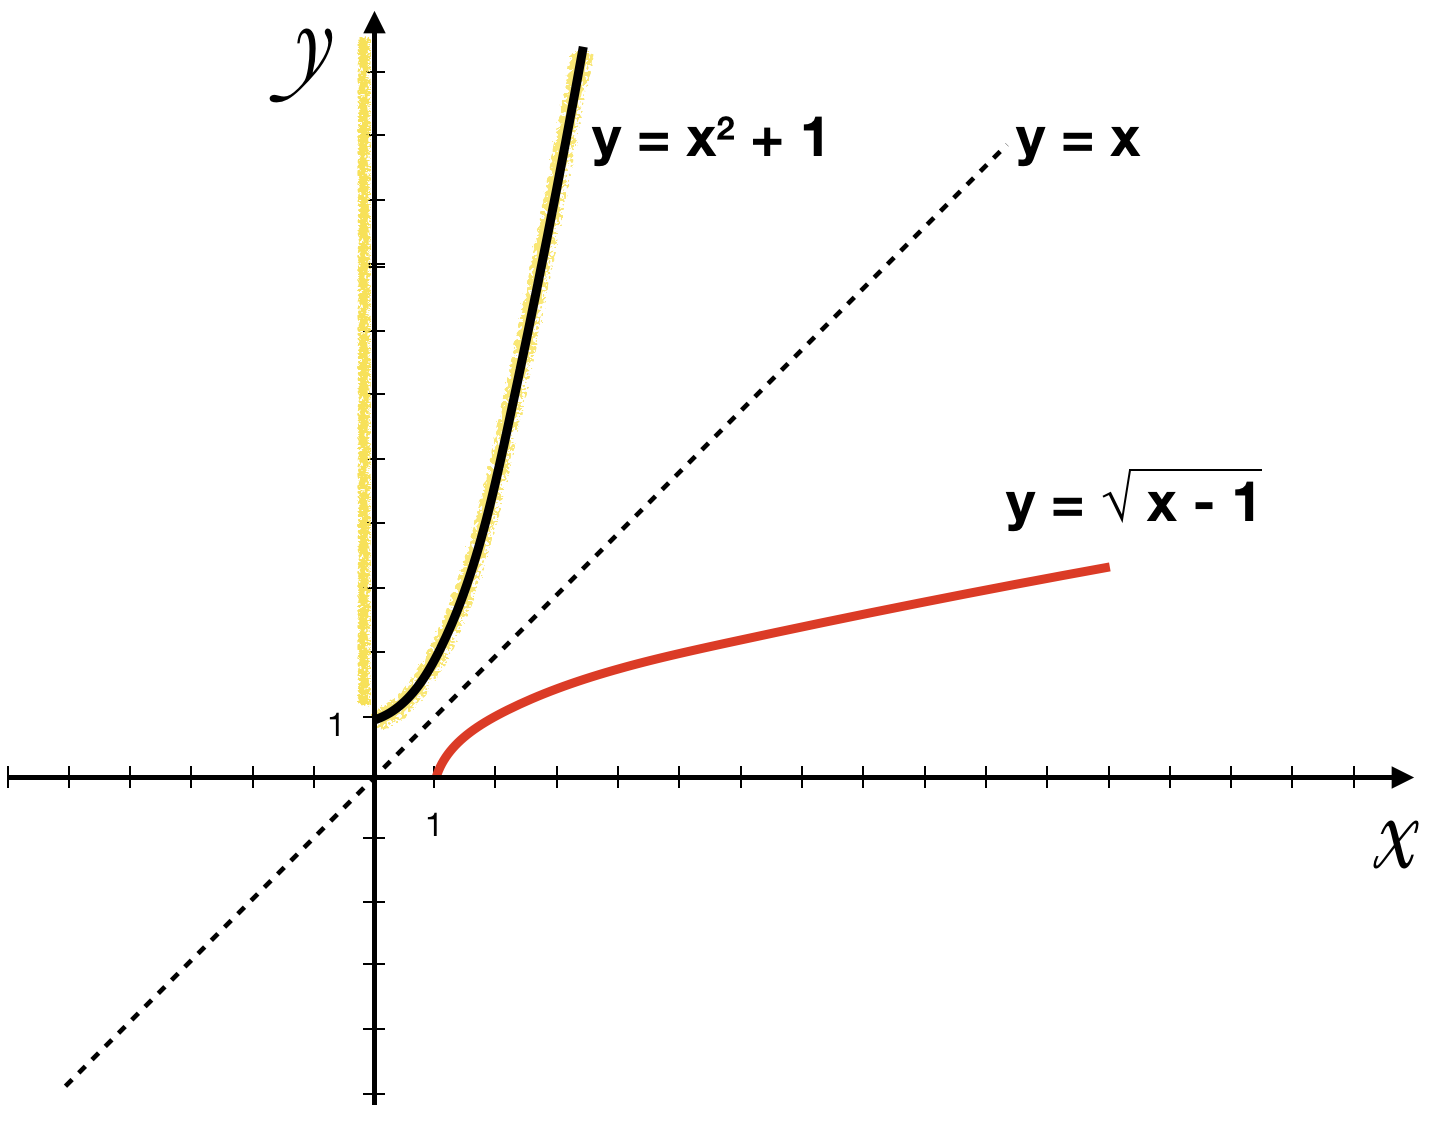
\includegraphics[width=0.7\textwidth]{img/funz_14c.png} 
  %\caption{}
  %\label{fig:funz_14abc}
  \end{figure}
  \item Se $f$ non è biiettiva e quindi non è invertibile, possiamo 
operare una \textsc{restrizione del dominio} a un sottoinsieme in cui $f$ 
risulti biiettiva.
  \begin{figure}[htpb!]
  \centering
  
%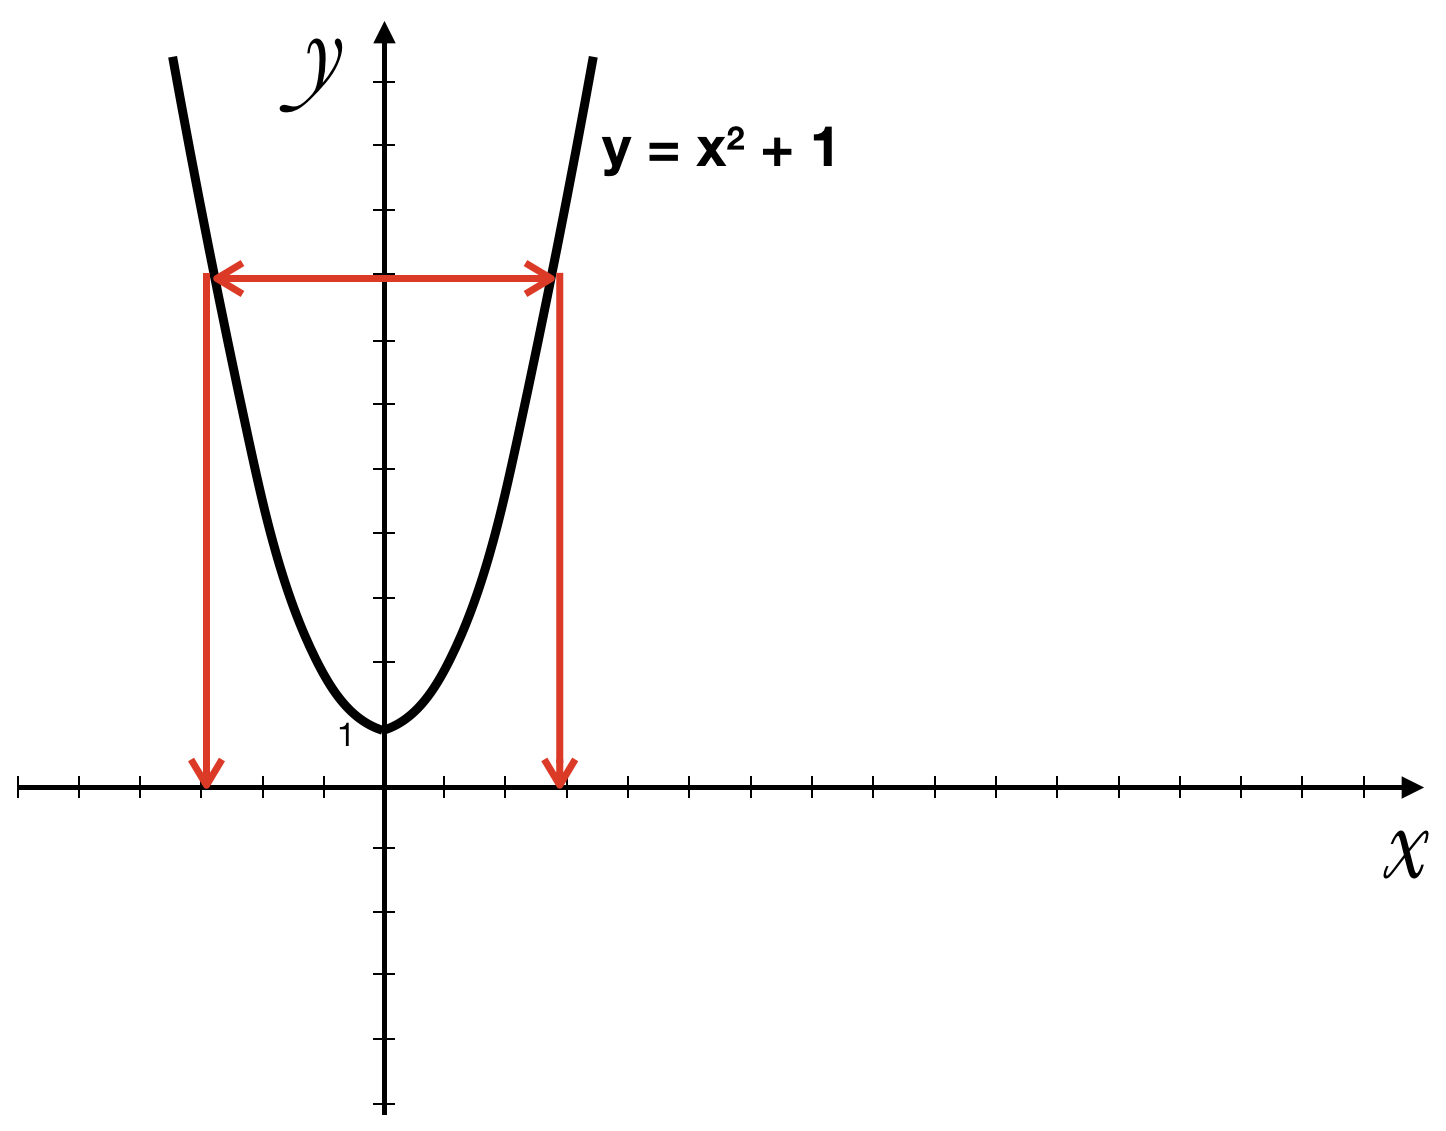
\includegraphics[width=0.7\textwidth]{img/funz_14a.png} %\quad
  
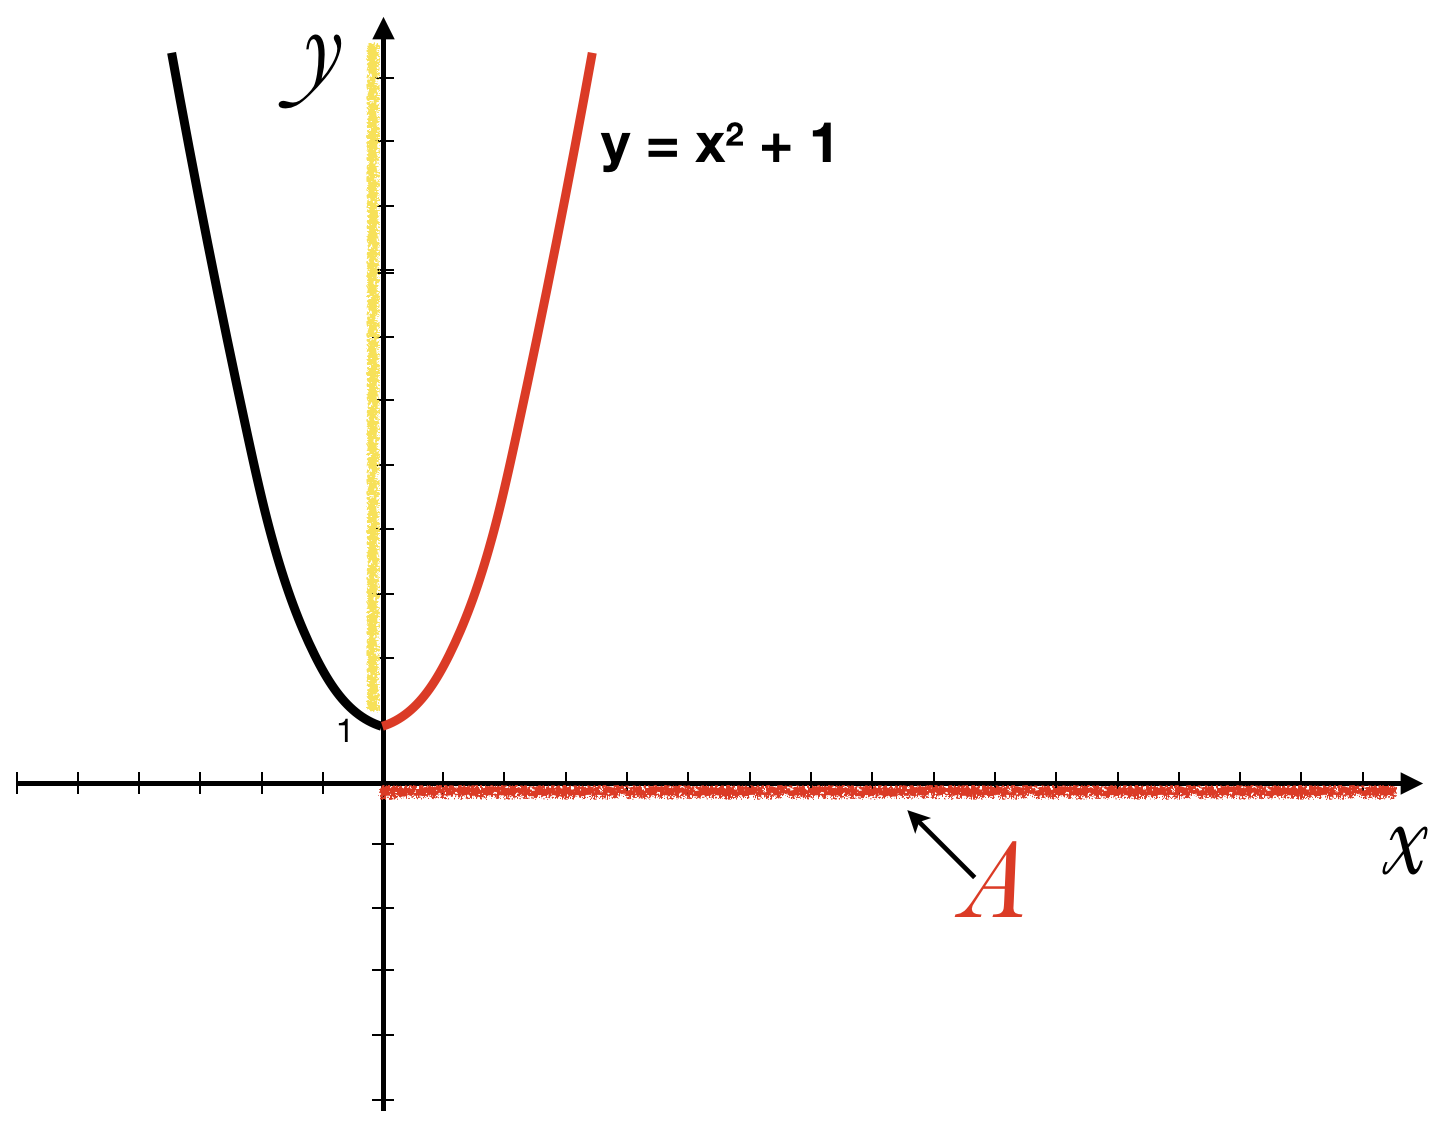
\includegraphics[width=0.45\textwidth]{img/funz_14b.png} %\quad
  
%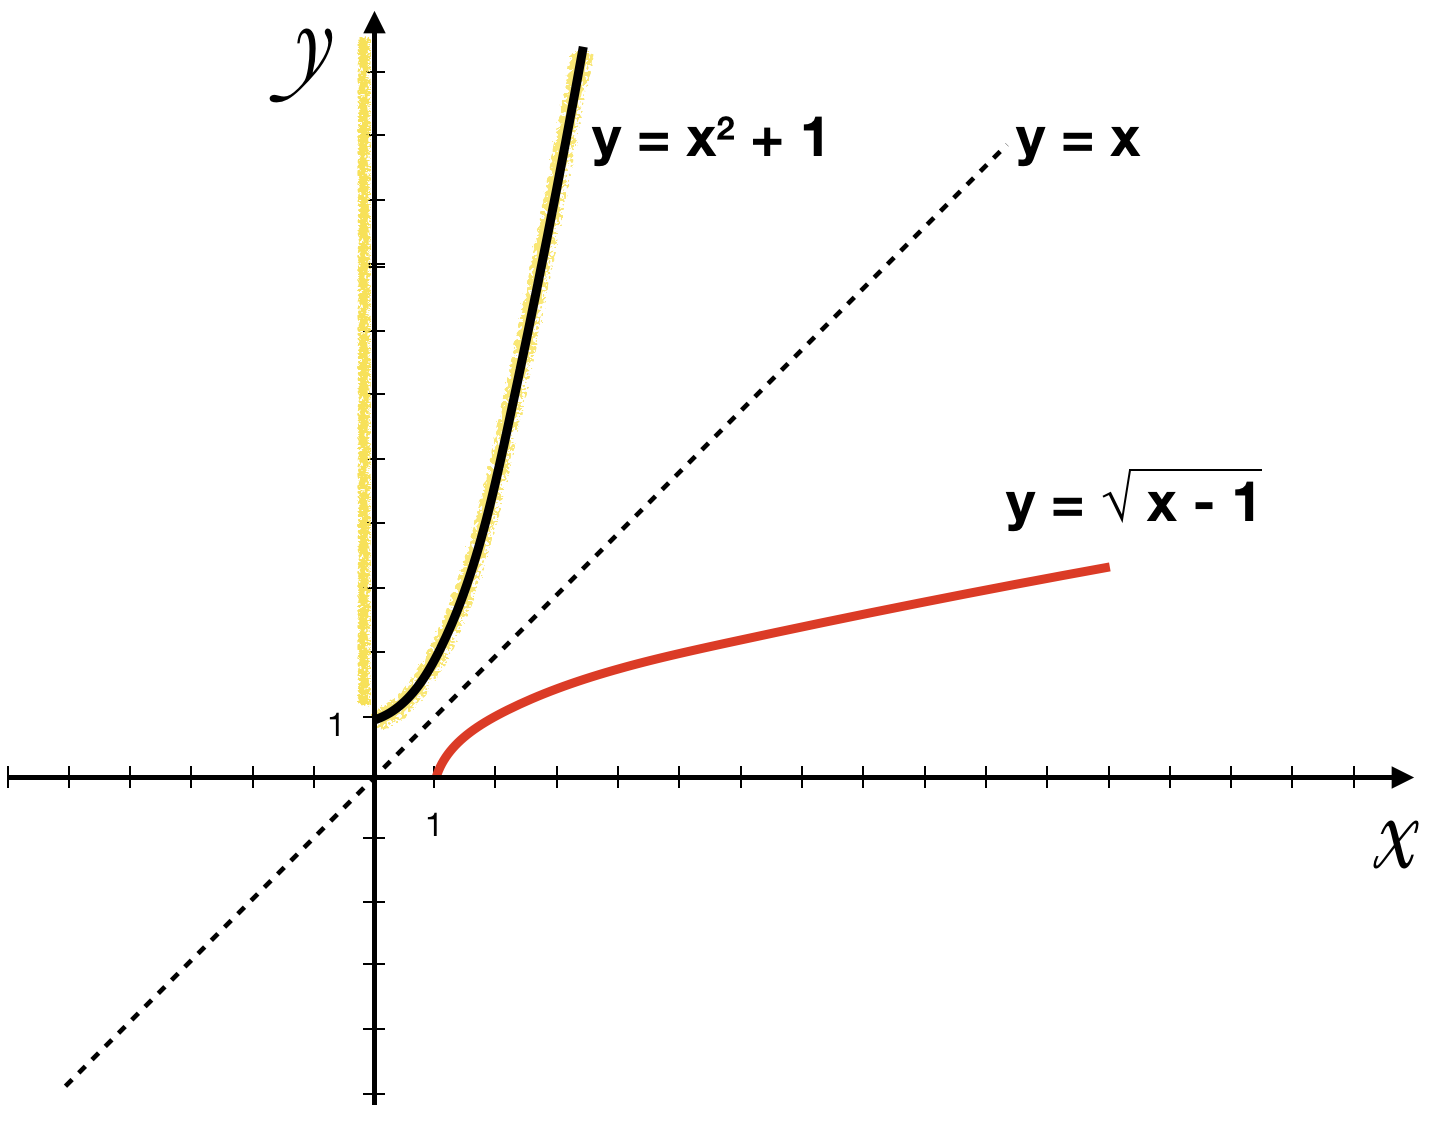
\includegraphics[width=0.7\textwidth]{img/funz_14c.png} 
  %\caption{}
  %\label{fig:funz_14abc}
  \end{figure}
  \item Scelgo solo una parte del dominio che chiamo $A$ e disegno 
l'inversa riflettendo la porzione di funzione biiettiva rispetto alla 
bisettrice del primo e terzo quadrante, la retta di equazione $y=x$.
  \begin{figure}[htpb!]
  \centering
  
%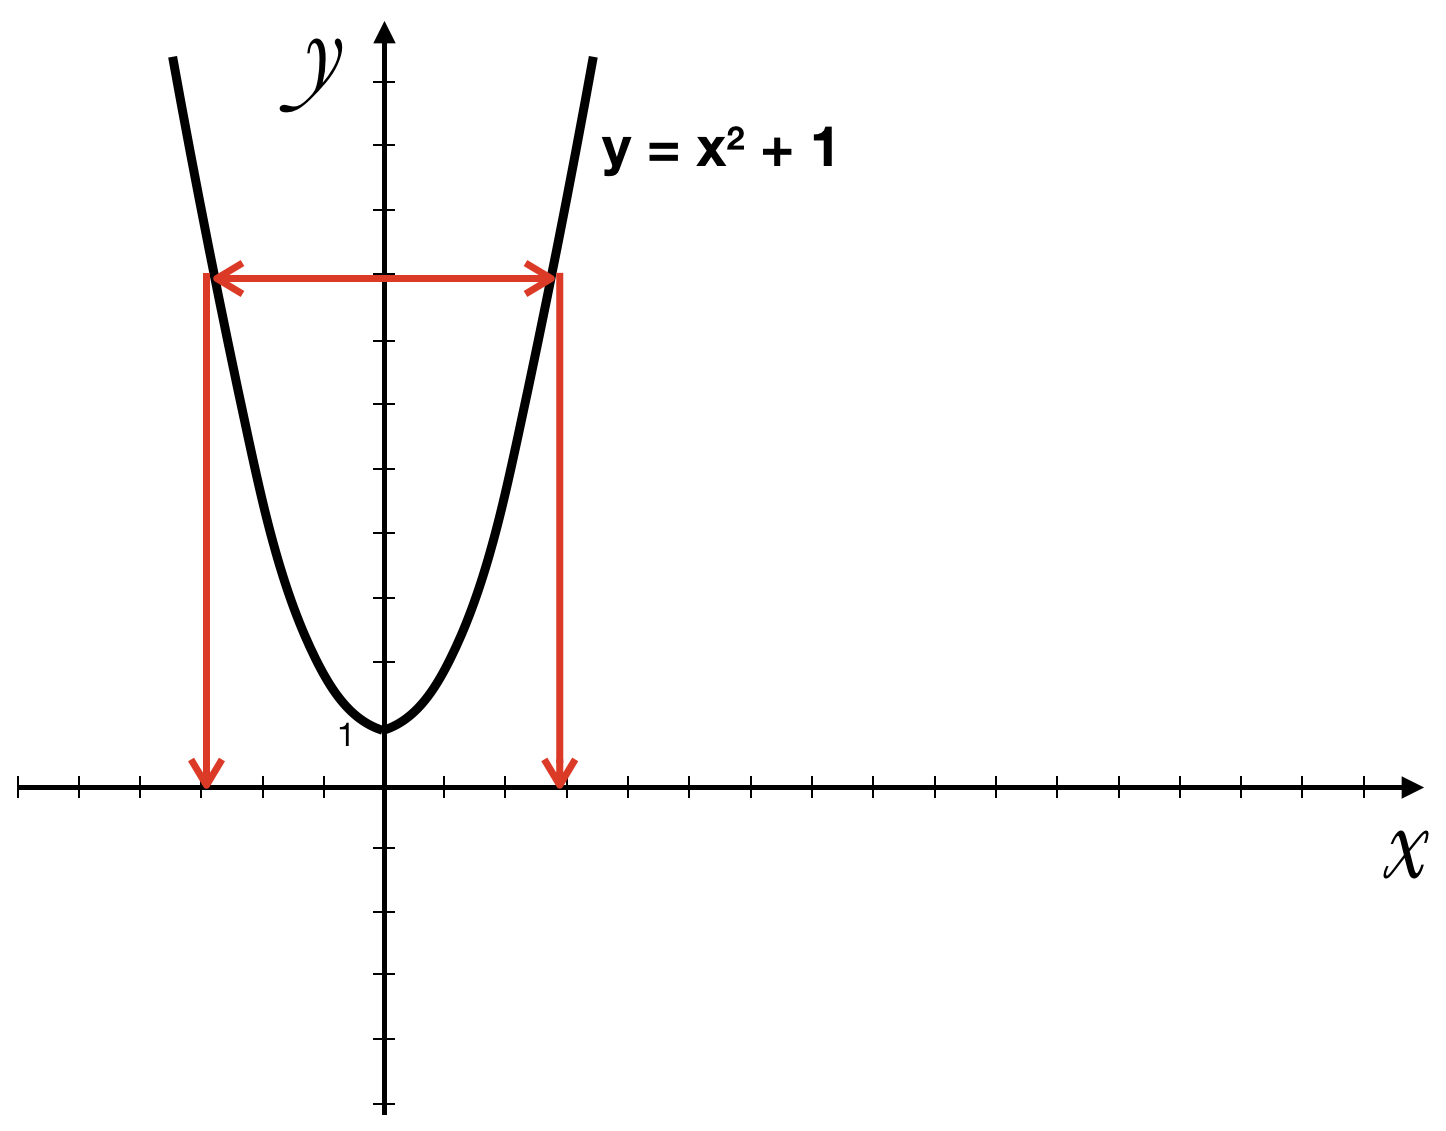
\includegraphics[width=0.7\textwidth]{img/funz_14a.png} \quad
  
%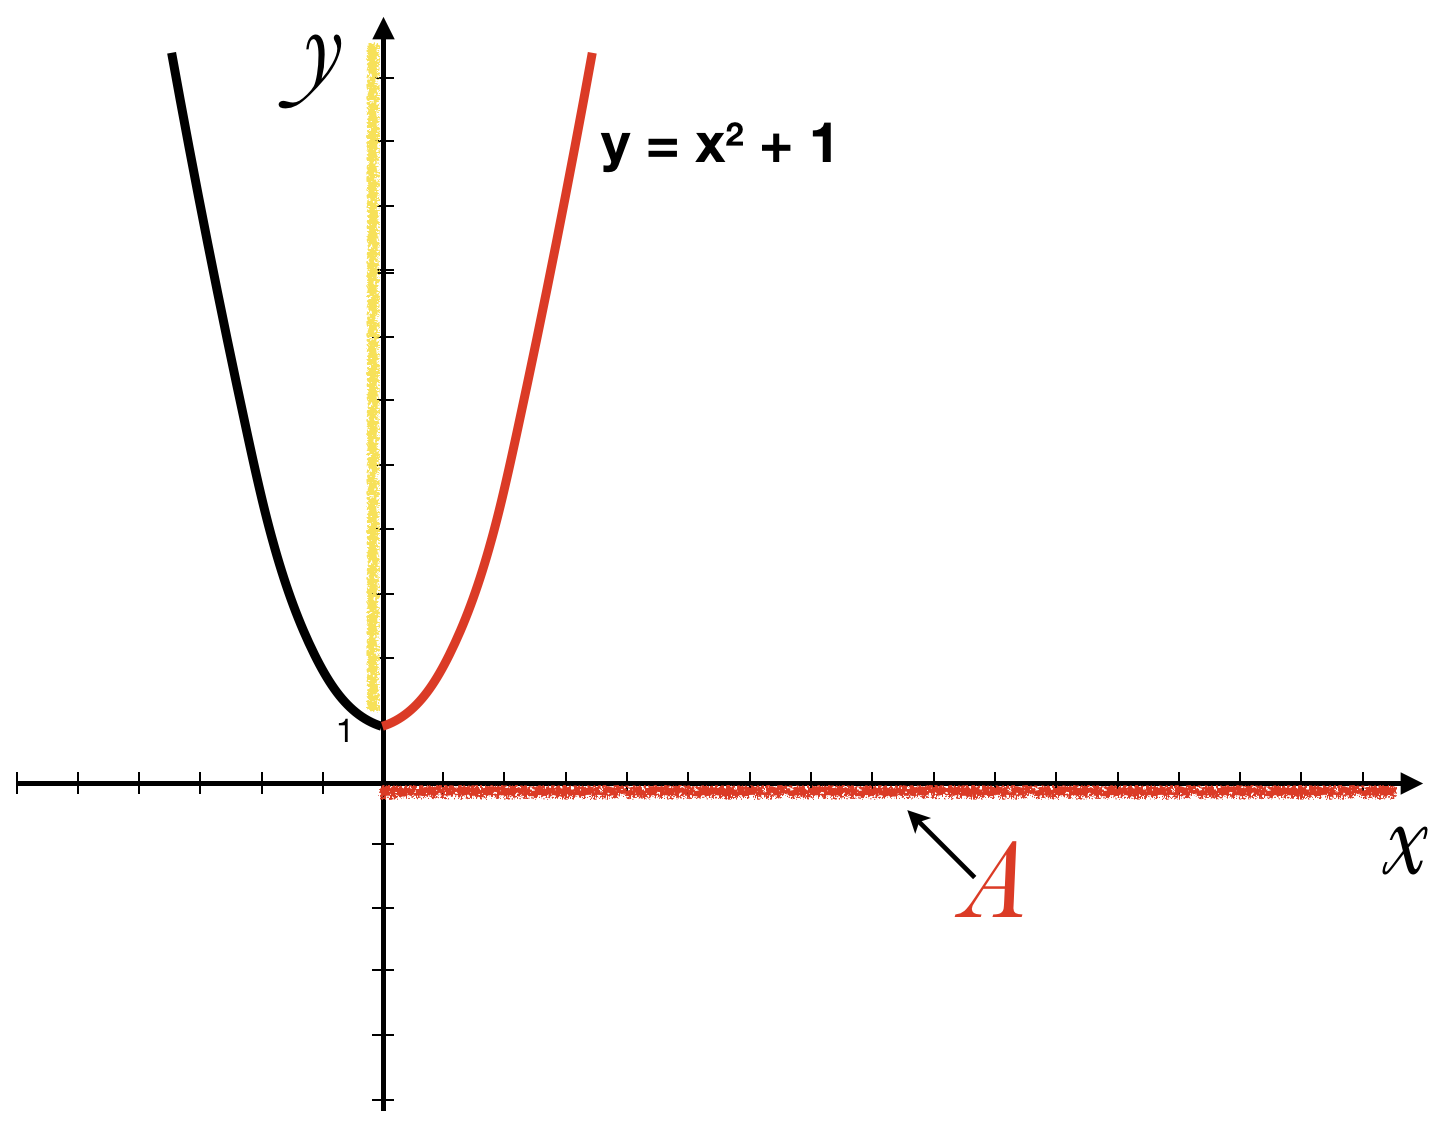
\includegraphics[width=0.7\textwidth]{img/funz_14b.png} %\quad
  
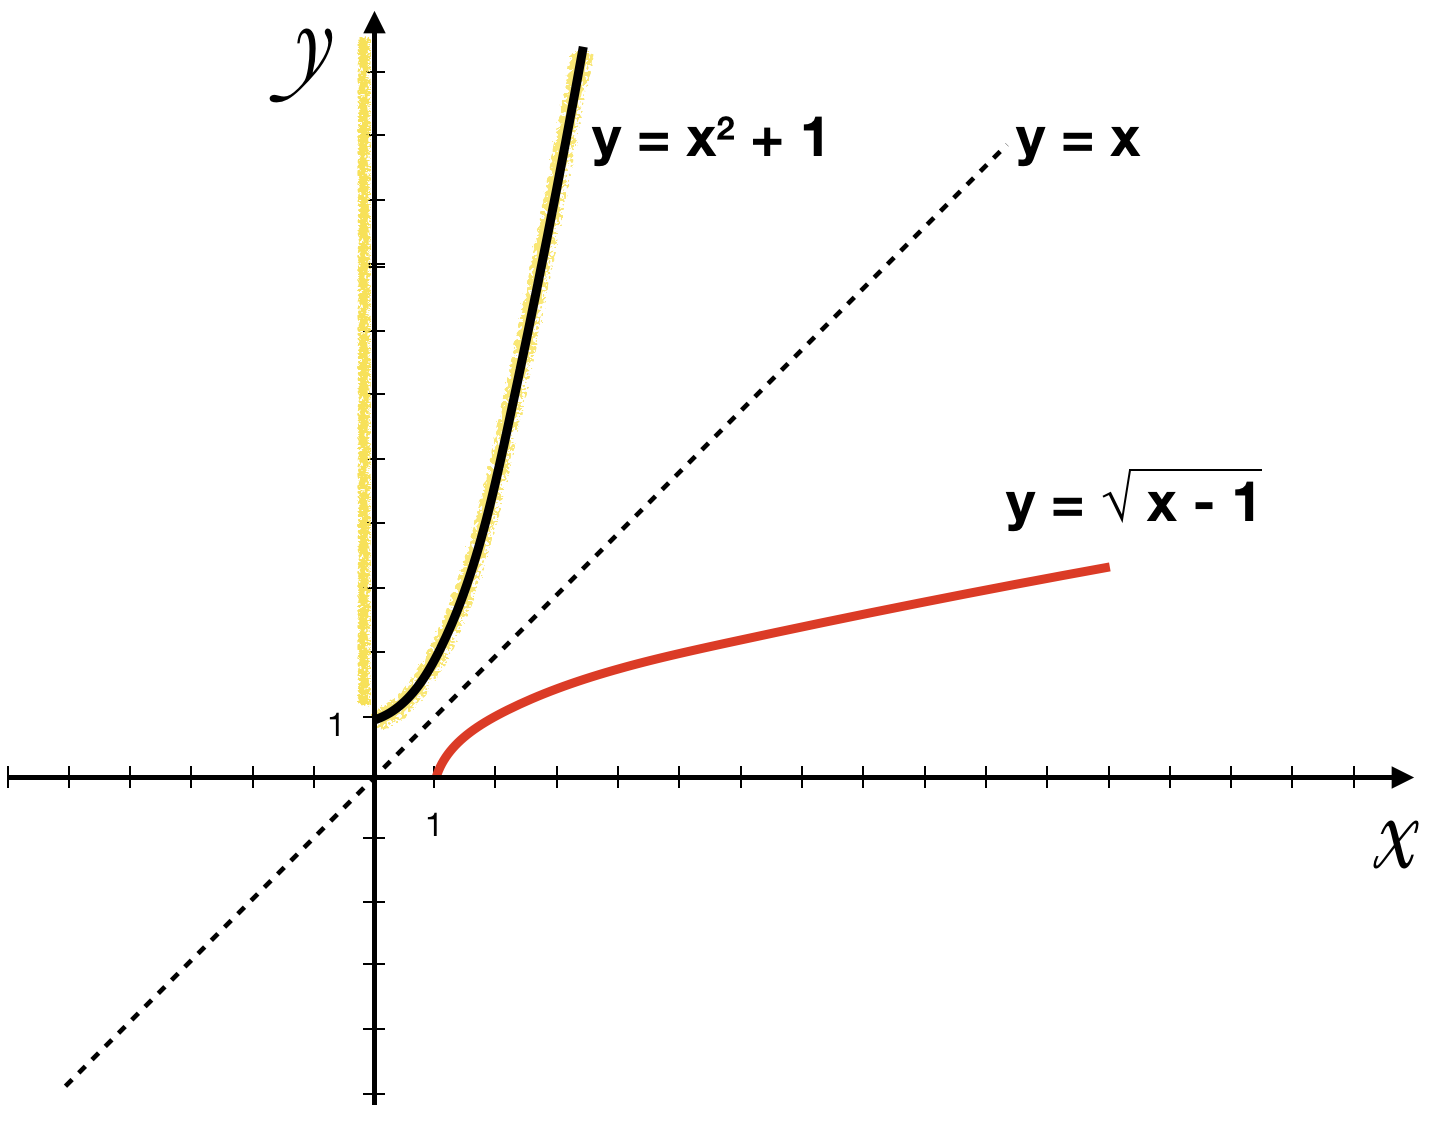
\includegraphics[width=0.45\textwidth]{img/funz_14c.png} 
  %\caption{}
  %\label{fig:funz_14abc}
  \end{figure}
\end{itemize}
\end{esempio}

Come visto negli esempi precedenti, il grafico della funzione $f^{-1}$, 
inversa della funzione $f$, è il simmetrico di $f$ rispetto alla bisettrice 
del primo e terzo quadrante.\\

Anche se sappiamo che l'inversa di una certa funzione deve essere simmetrica 
rispetto ad essa, trovare l'inversa di una determinata funzione e in 
particolar modo la sua forma analitica può non essere immediato. Forniamo 
quindi una procedura.\\

%\begin{procedura}
\textbf{Procedura 1.1} Determinare l'inversa di una funzione data:% 
\textcolor{blue}{[vedi la procedura a pag 100 vol3]}
\begin{enumerate}
  \item Si verifica che $f(x)$ è invertibile;
  \item Si esplicita la $f$ rispetto a $x$;
  \item Nella forma appena trovata si sostituisce $x$ con $y$ e $y$ con 
$x$.
\end{enumerate}
%end{procedura}
  
\begin{esempio}
Invertiamo la funzione: $f(x)=y=\sqrt[3]{x}-1$
\begin{enumerate}
  \item La funzione è invertibile perché è strettamente crescente in 
tutto il dominio $\mathbb{R}$.
  \item Esplicitiamo la funzione rispetto a $x$:\\
   $y=\sqrt[3]{x}-1\rightarrow y+1=\sqrt[3]{x}\rightarrow(y+1)^3=x$
  \item Infine otteniamo: $f^{-1}(x)=y=(x+1)^3$
\end{enumerate}
\end{esempio}

\begin{esempio}
Invertiamo la funzione: $f(x)=y=e^{x+1}-1$
\begin{enumerate}
  \item La funzione è invertibile perché è strettamente crescente in 
$\mathbb{R}$.
  \item Esplicitiamo la funzione rispetto a $x$:\\
   $y=e^{x+1}-1\rightarrow y+1=e^{x+1}\rightarrow 
\ln(x+1)=\ln(e^{x+1})\rightarrow \ln(y+1)-1=x$.\item Infine otteniamo: 
$f^{-1}(x)=y=\ln(x+1)-1$.
\end{enumerate}
\end{esempio}

Studiate le funzioni inverse discutiamo ora un'operazione tra funzioni che ci 
consentirà di creare funzioni complesse a partire da funzioni semplici: 
questa operazione si chiama \textsc{composizione di funzioni} e il suo 
risultato sarà una nuova funzione detta composta.\\

%
\begin{definizione} 
Date le funzioni $f : A\to B$ e $g : B\to C$ si dice funzione composta 
$f\circ g$ la funzione:   $(g\circ f)(x)=g(f(x))$ che associa ad ogni 
elemento di $A$ un elemento di $C$ in modo che
  \begin{itemize}
  \item all'elemento $x\in A$ corrisponde mediante $f$, 
l'elemento $f(x)\in B$
  \item all'elemento $f(x)\in B$ corrisponde, mediante $g$, 
l'elemento $g(f(x))\in C$
  \end{itemize}
affinché sia possibile calcolare $g(f(x))$, $f(x)$ deve appartenere al 
dominio di $g$. Il dominio di $g\circ f$ è costituito da tutti gli elementi 
del dominio di $f$ tali che $f(x)$ appartiene al dominio di $g$.
\end{definizione}

\begin{figure}[htpb!]
  \centering
  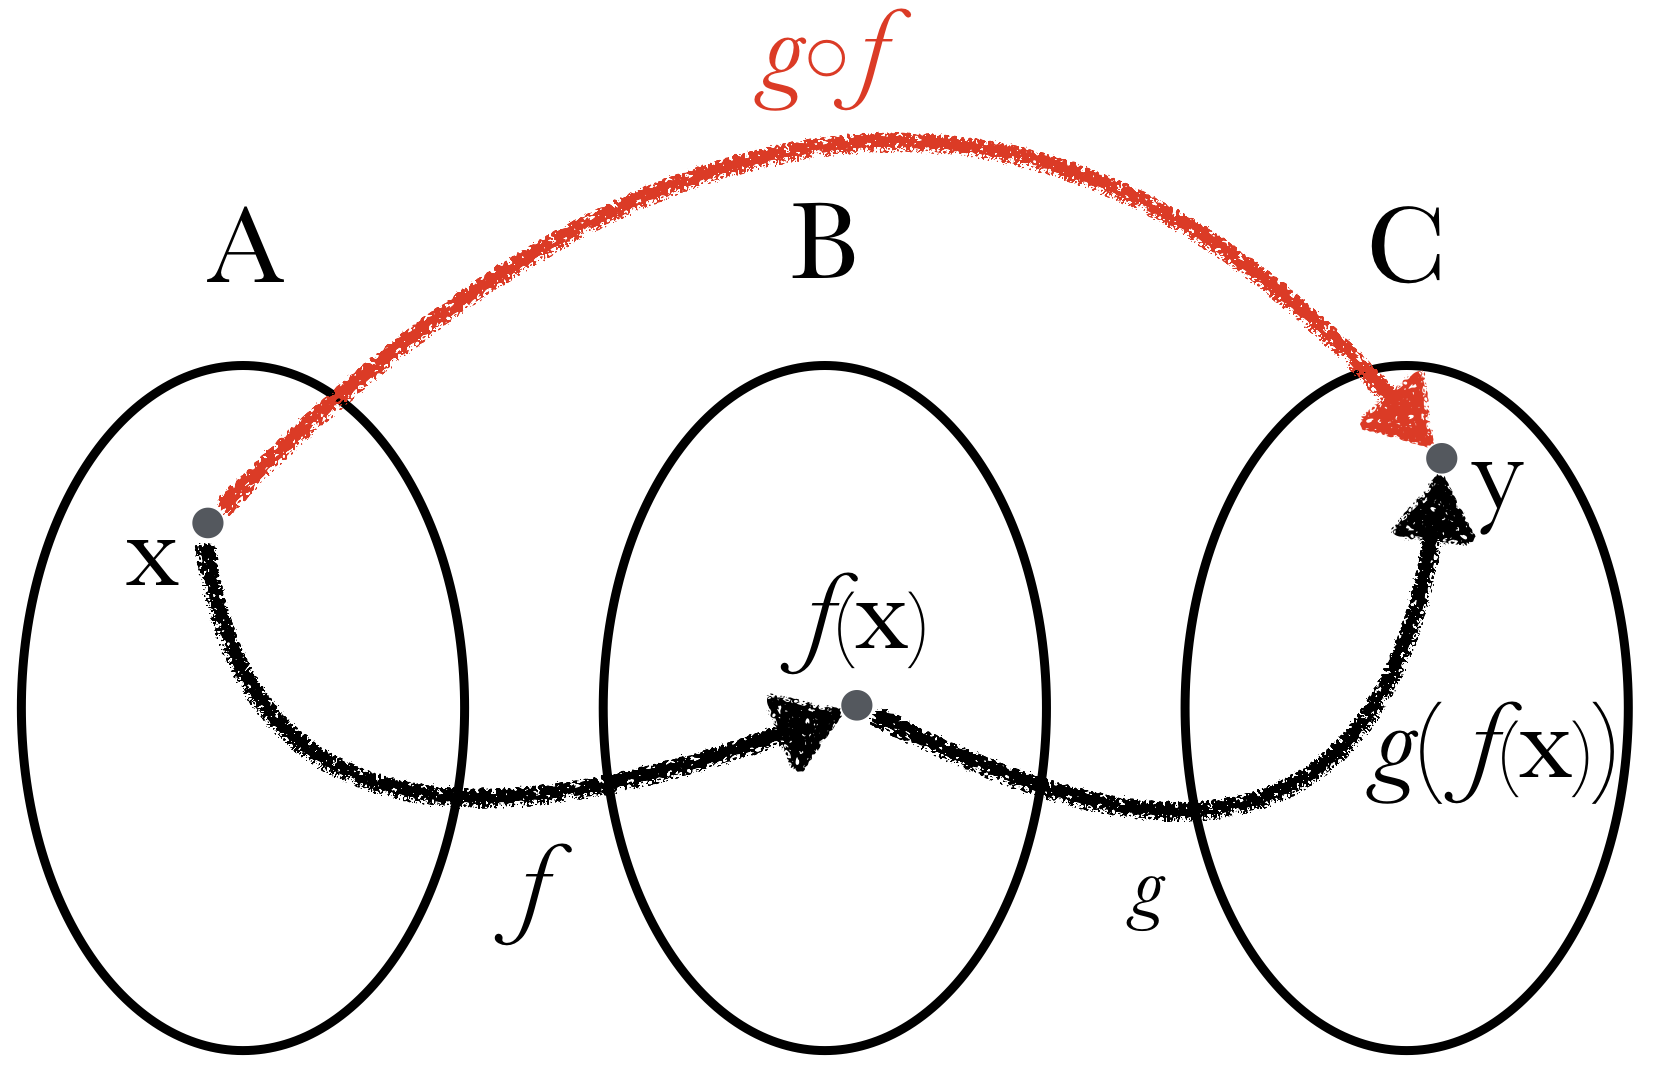
\includegraphics[width=0.55\textwidth]{img/funz_15.png} 
  %\caption{}
  %\label{fig:funz_14abc}
\end{figure}
%

La simbologia $g\circ f$ si legge <<$g$ composto $f$>> o <<$g$ dopo $f$>>; 
$g(f(x))$ si legge <<$g$ di $f$ di $x$>>.\\
 
Per quanto riguarda le proprietà di questa operazione tra funzioni notiamo 
che la composizione è associativa: $(f\circ g)\circ h=f\circ (g\circ h)$, ma 
in generale non commutativa $g\circ f\neq f\circ g.$ \\

\begin{esempio} 
Date le due funzioni $f(x)=\sqrt{x}$ e $g(x)= x+5$, determiniamo le funzioni 
composte $g\circ f$ e $f\circ g$.
Abbiamo $g\circ f=g(f(x))=g(\sqrt{x})=\sqrt{x}+5$ e il dominio  della 
funzione ottenuta è $x\geq0$. Otteniamo l'altra composta con un procedimento 
analogo $f\circ g=f(g(x))=f(x+5)=\sqrt{x+5}$ e il suo dominio è $x\geq5$. La 
diversità delle due funzioni ottenute ci conferma la non commutatività 
dell'operazione di composizione.\\
\end{esempio}

\textbf{Posso comporre una funzione con la sua inversa?}\\
Sia $f$ una funzione invertibile di dominio $D$ e immagine $I$, con $f^{-1} $ 
la sua inversa.
Consideriamo la composta $f^{-1}\circ f$, cioè $f^{-1}$ dopo $f$: $x$ va in 
$f(x)$ che a sua volta va in $x$, $f^{-1}(f(x))=x$, $\forall x\in D$ 
$f^{-1}\circ f$ è la funzione identità in $D$, analogamente anche 
$f(f^{-1}(x))=x$, $f\circ f^{-1}$ è l'identità in $I$. Ricordiamo che la 
funzione identità è una particolare funzione che associa ad ogni $x$ la $x$ 
stessa, cioè associa ad ogni elemento del dominio, lo stesso elemento nel 
codominio.\\

\begin{definizione}
Due funzioni $f$ e $g$ si dicono uguali se hanno lo stesso dominio $D$ e 
risulta $$f(x)=g(x)$$ $\forall x\in D$.\\
\end{definizione}
 
\begin{esempio}
Vediamo un esempio di funzioni uguali e non uguali. Le due funzioni
$$f(x)=\frac{\sqrt{x}}{\sqrt{x^2+4}}$$ e $$g(x)=\sqrt{\frac{x}{x^2+4}}$$
sono uguali perchè hanno lo stesso dominio ($x\geq0$) e risulta:
$$\frac{\sqrt{x}}{\sqrt{x^2+4}}=\sqrt{\frac{x}{x^2+4}}$$ per ogni $x\geq0$.
Vediamo un contoesempio di funzioni uguali. Le due funzioni
$$f(x)=\frac{\sqrt{x}}{\sqrt{x+4}}$$ e $$g(x)=\sqrt{\frac{x}{x+4}}$$
non sono uguali perché hanno dominio diverso: la funzione $f$ è definita per 
$x\geq0$, mentre la funzione $g$ è definita per $x<-4\lor x\geq 0$.
$$\frac{\sqrt{x}}{\sqrt{x^2+4}}=\sqrt{\frac{x}{x^2+4}}$$ per ogni $x\geq0$.
\end{esempio}

%\section{Simmetrie e grafici deducibili}
%label{}
\newpage 
\section{Esercizi}
%label{}
  \subsection{Esercizi dei singoli paragrafi}
  %label{}
  \subsubsection*{1.1 Definizione di funzione}
  %label{}
  \begin{itemize}
  \item[1.1)] Riflettendo sulla definizione di 
funzione rispondi argomentando alle seguenti domande:
  \begin{itemize}
  \item[a)] Quali tra i 
seguenti oggetti, che puoi rappresentare sul piano cartesiano, è una 
funzione: circonferenza, ellisse, parabola con asse verticale?
  \item[b)] Quali tra i 
seguenti oggetti, che puoi rappresentare sul piano cartesiano, sono funzioni: 
retta verticale, retta orizzontale, retta obliqua?
  \item[c)] Considera una 
parabola con asse verticale e una con asse orizzontale, quale delle due è una 
funzione?
  \end{itemize}
  \item[1.2)] Determina il dominio delle 
seguenti funzioni
  \begin{itemize}
  \item[a)] $y= 4x^2+x+2$   
   \hfill  [ $D=R$ ]
  \item[b)] 
$y=\frac{3x+2}{x-5}$   \hfill   
   [ $D=R-\{5\}$ ]
  \item[c)] $y=\sqrt{9-x^2}   $ 
   \hfill   [ $D=[-3, 3]$ ]
  \item[d)] 
$y=\frac{4x}{\sqrt{x+2}}  $  \hfill   
   [ $D=]-2,+\infty[$ ]
  \item[e)] 
$y=\frac{2+3x}{x^2+7x+12}$   \hfill   
[$D=\mathbb{R}-\{-3,-4\}$]
  \item[f)] $y=e^{x+3}$\hfill   
   [$D=\mathbb{R}$]
  \item[g)] $y=\log_2(x+3)$  
\hfill  [$D=]-3, +\infty[$ ]
  \item [h)] $y=\ln(x^2+6x+8)$  
  \hfill   
[$D=]-\infty,-4[\cup]-2,+\infty[$]
  
\item[i)]$y=\frac{x^3+3x}{e^x+5}$\hfill   
  [$D=\mathbb{R}$]
  
\item[l)]$y=\frac{3x^2+4}{e^x-2}$   \hfill  
   [$D=\mathbb{R}-\{\ln2\}$]
  \item[m)] 
$y=\frac{4x-5}{2x-8}-\sqrt{x+3}$  \hfill  
[$D=[-3,4[\cup]4,+\infty[$]
  \item[n)]$y=\sqrt{\log(x+4)}$ 
   \hfill  [$D=[-3,+\infty[$]
  \item[o)]$y=(x+5)^{x+3}$  
   \hfill  [$D=]-5,+\infty[$]
  \item[p)] 
$y=2\sin{x}+\cos{2x}$   \hfill   
[$D=\mathbb{R}$]
  
\item[q)]$y={2+\cos{3x}}{2\sin{x}}$   \hfill  
   [$D=\mathbb{R}-\{k\pi,\,k\in \mathbb{Z}\}$]
  \item[r)] $y=\arcsin(x+2)$  
   \hfill  [$D=[-3, -1]$]
  
\item[s)]$y=\arctan(\frac{3}{x+2}) $  \hfill  
   [$D=\mathbb{R}-\{-2\}$ ]\\

  \end{itemize}
  \item[1.3)] Dall'analisi visiva del grafico deduci il 
dominio e codominio della funzione.
  \begin{figure}[htpb!]
  \centering
  
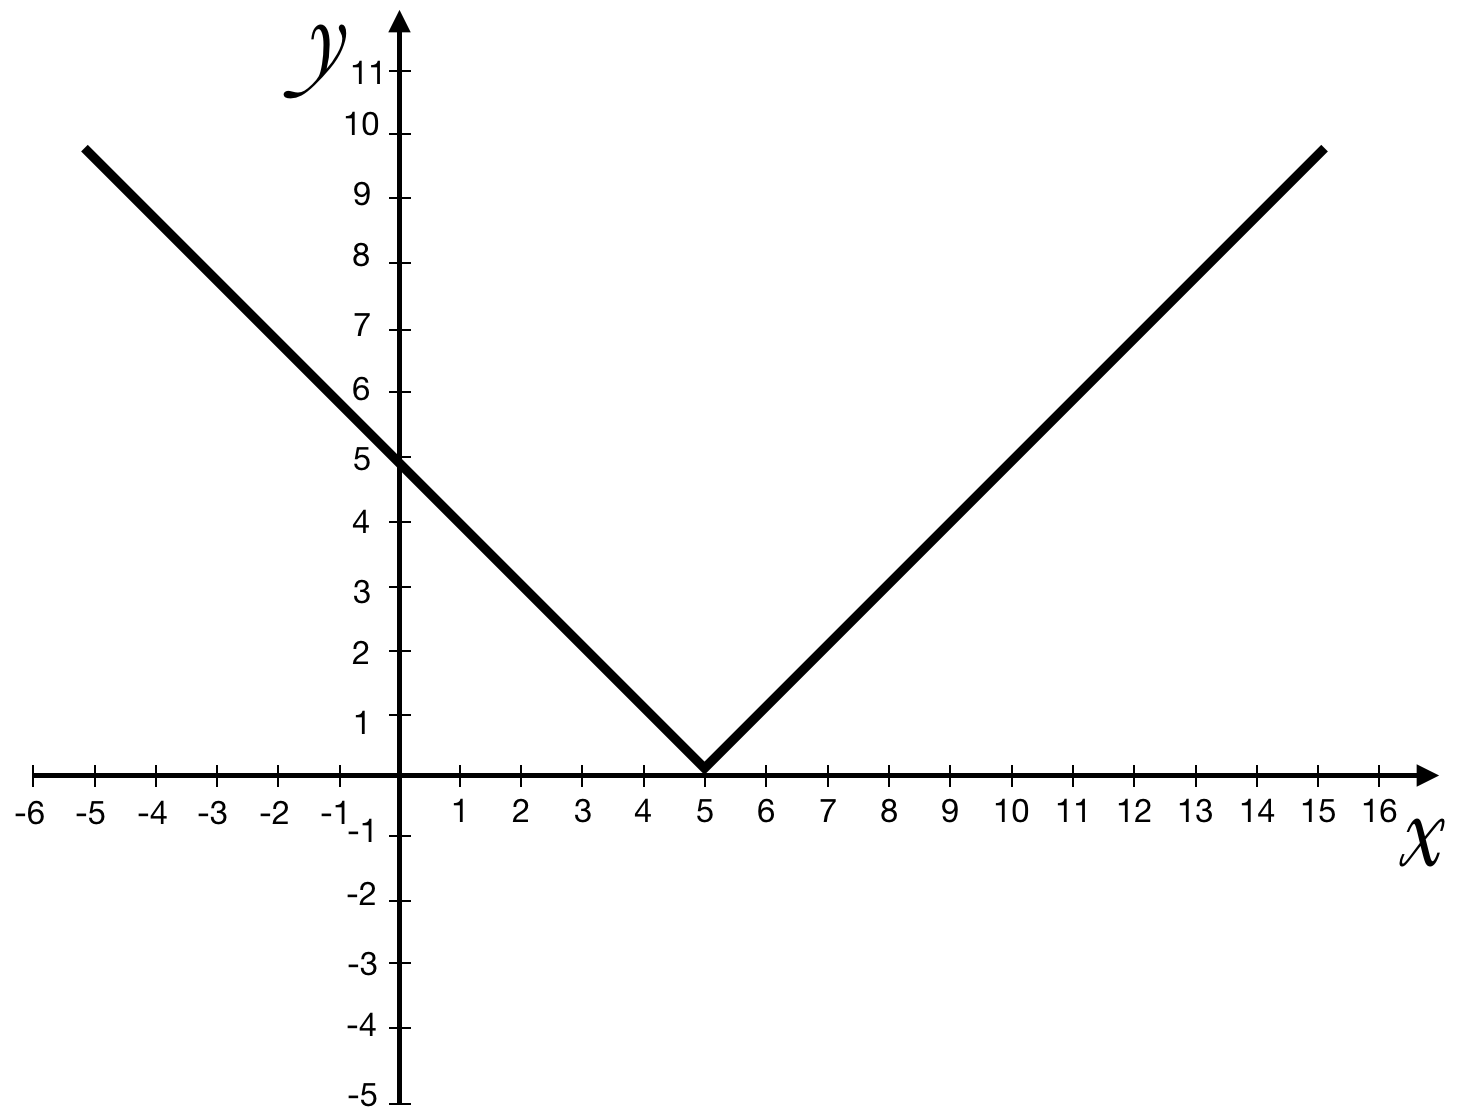
\includegraphics[width=0.45\textwidth]{img/funz_16.png}\quad  
  
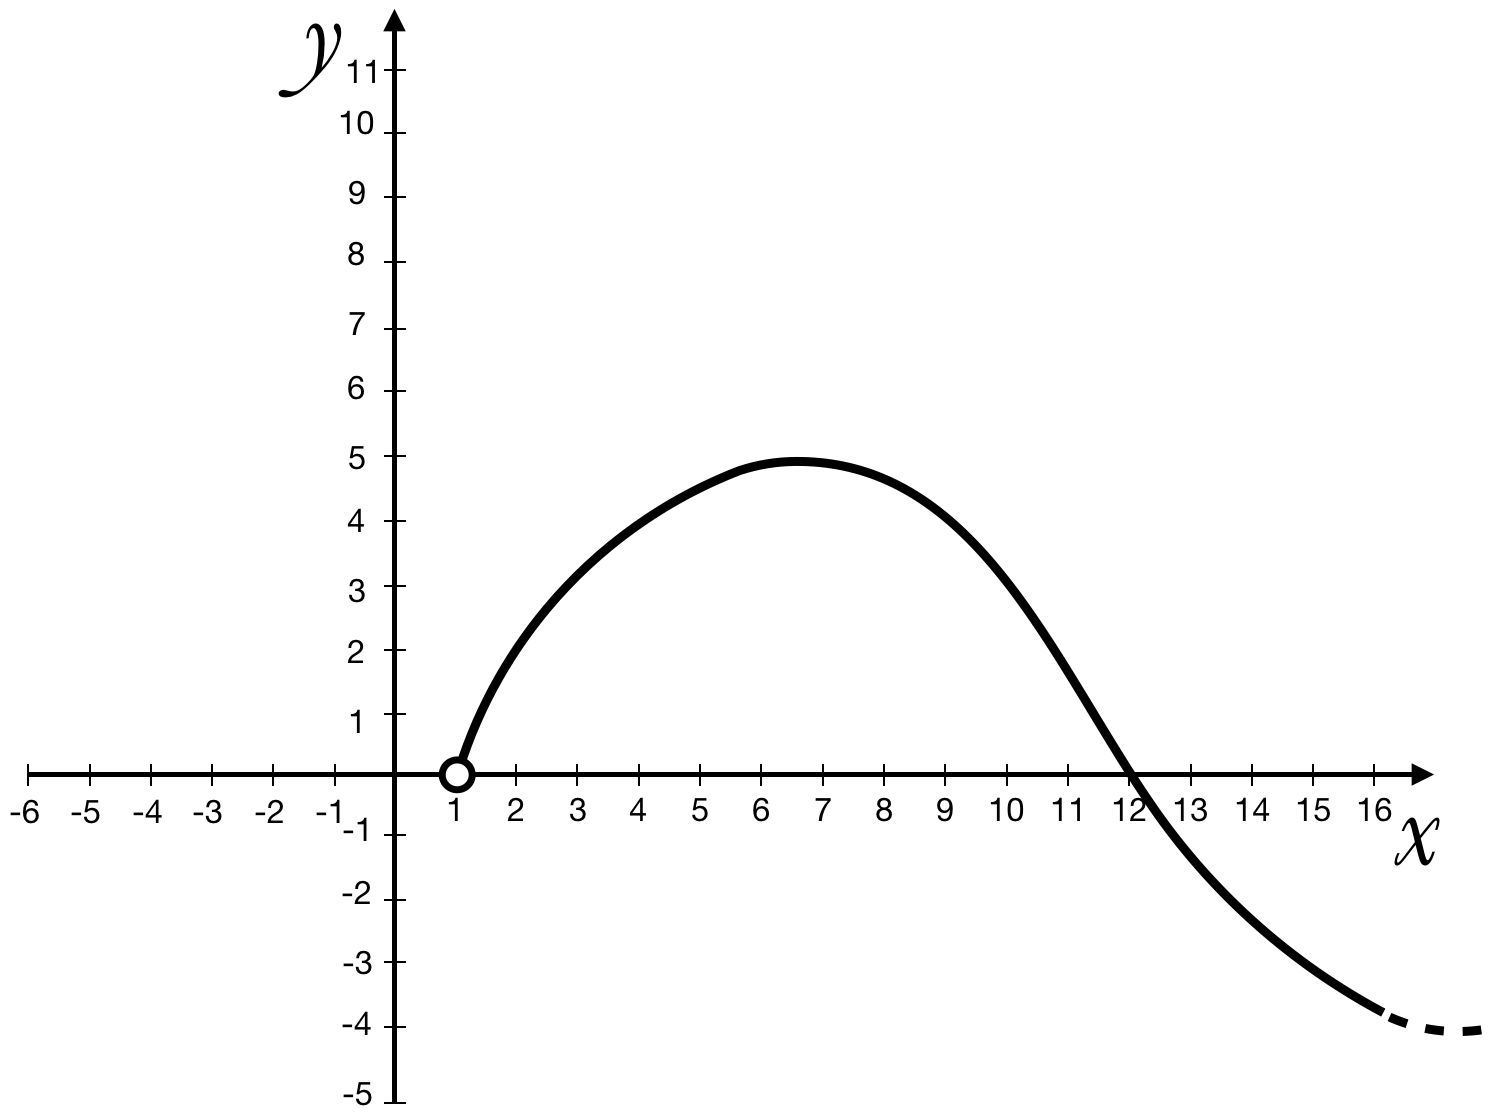
\includegraphics[width=0.5\textwidth]{img/funz_17.png}  
  
\quad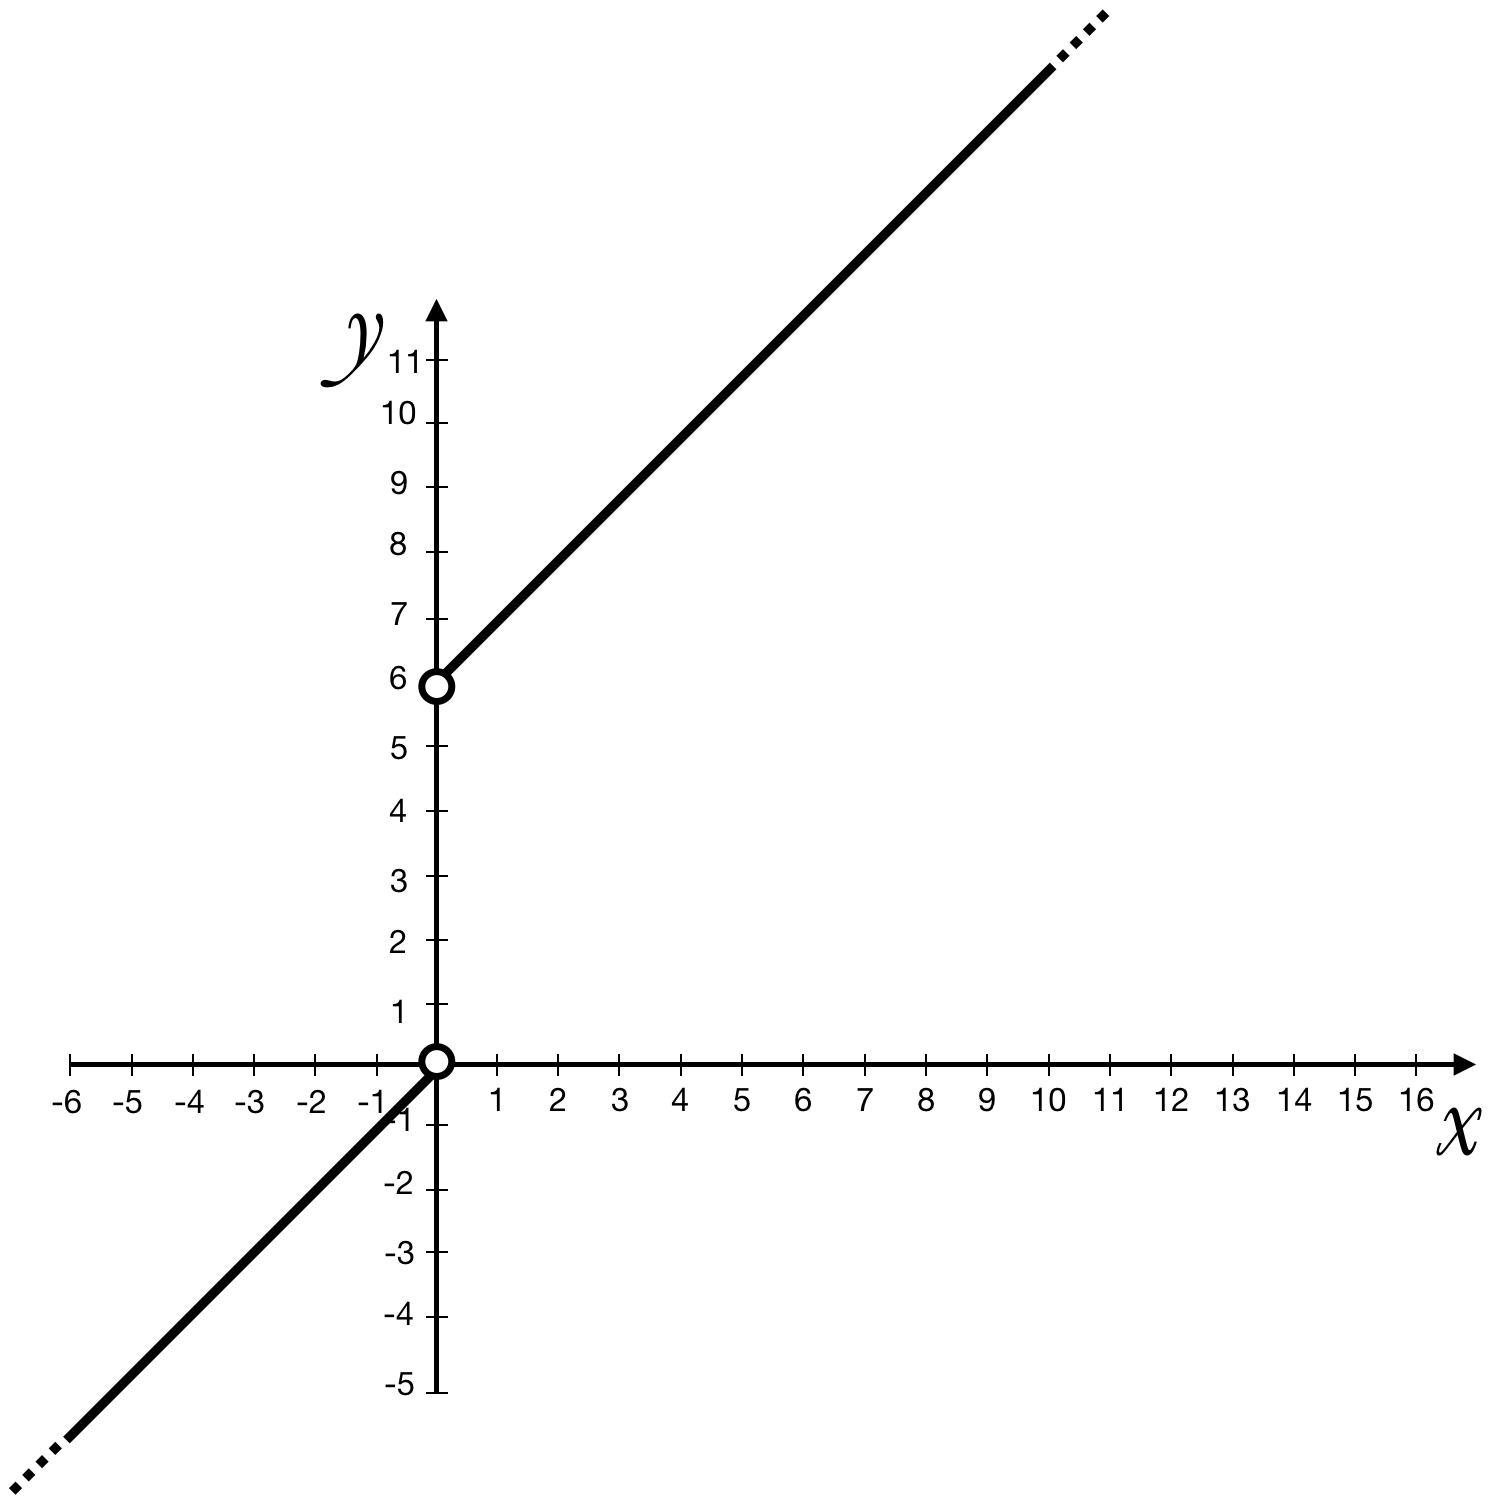
\includegraphics[width=0.45\textwidth]{img/funz_17a.png}   
  
\quad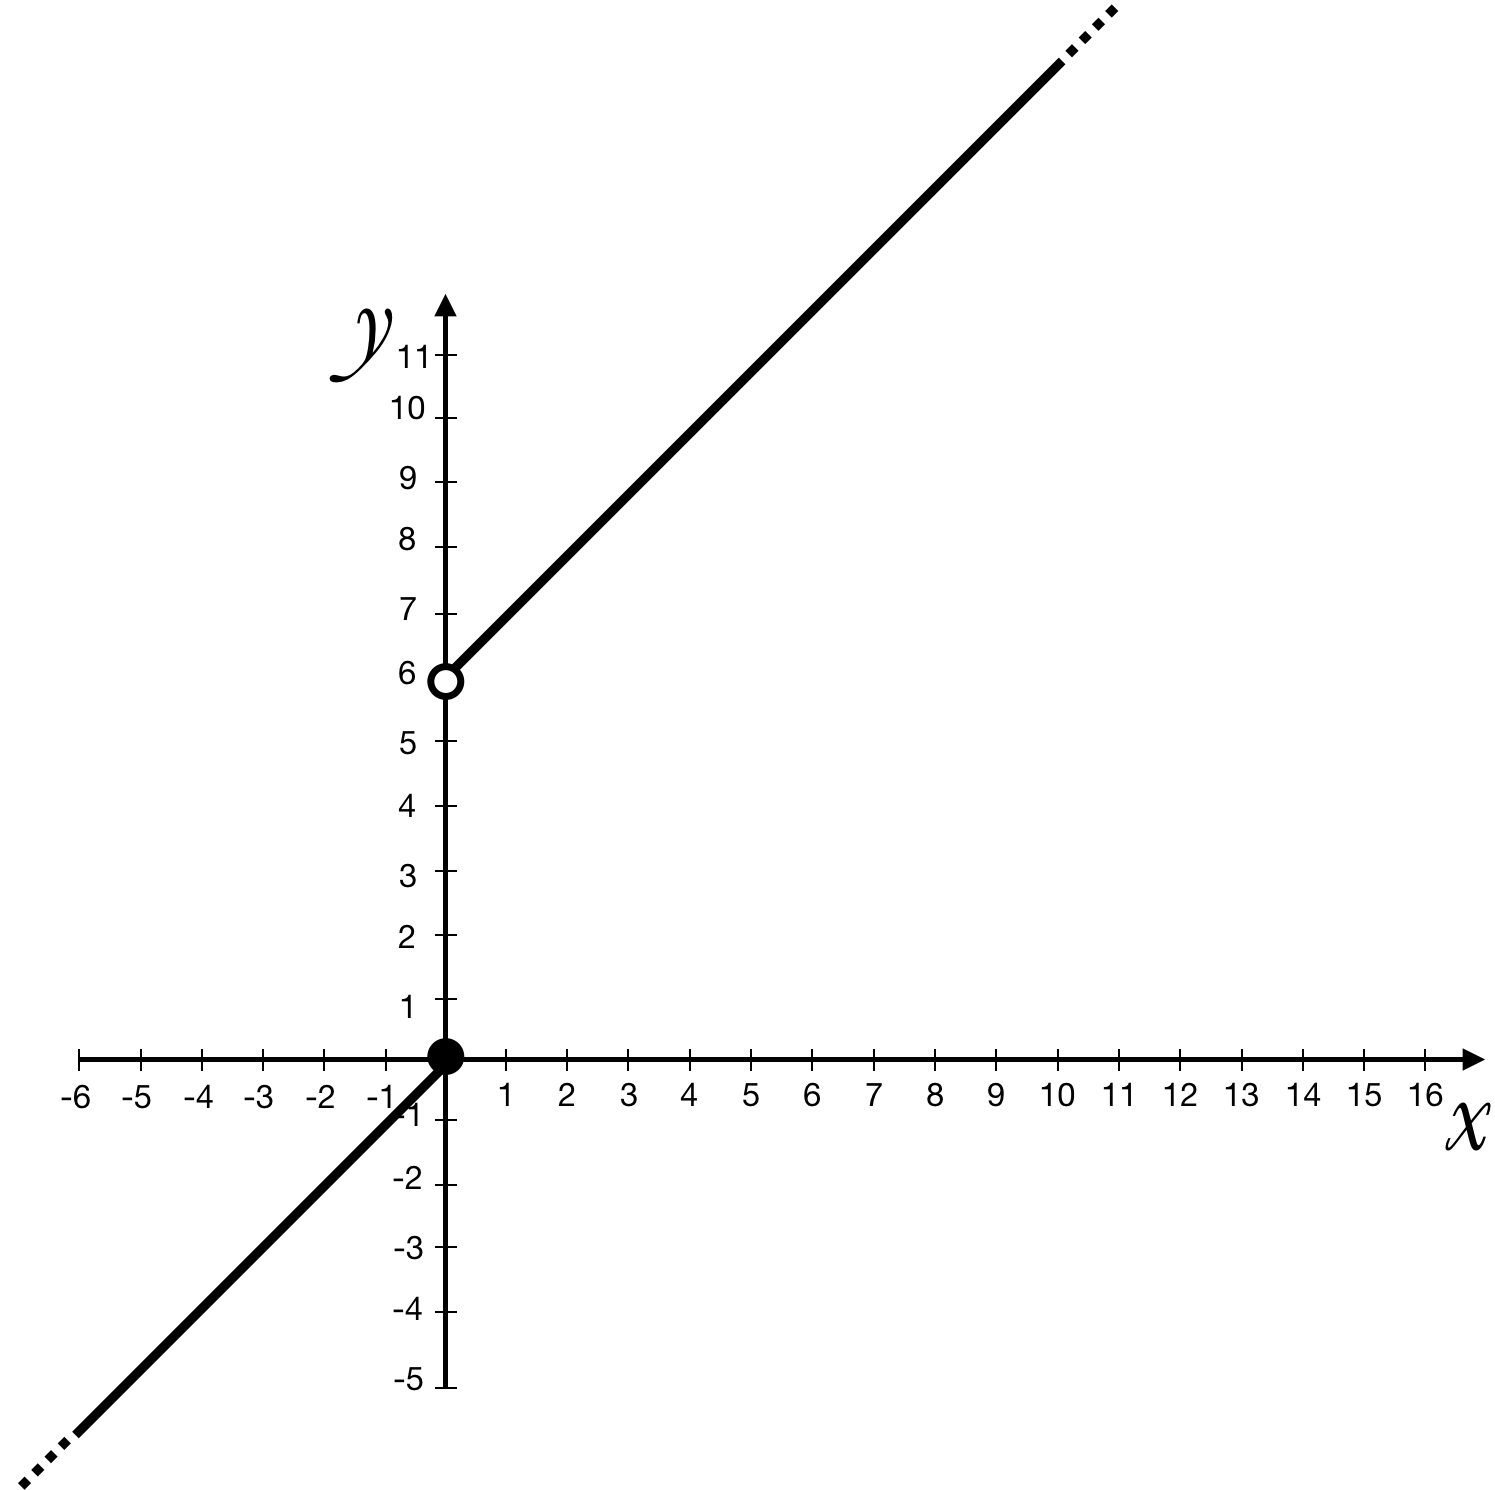
\includegraphics[width=0.45\textwidth]{img/funz_17b.png}   
  
\quad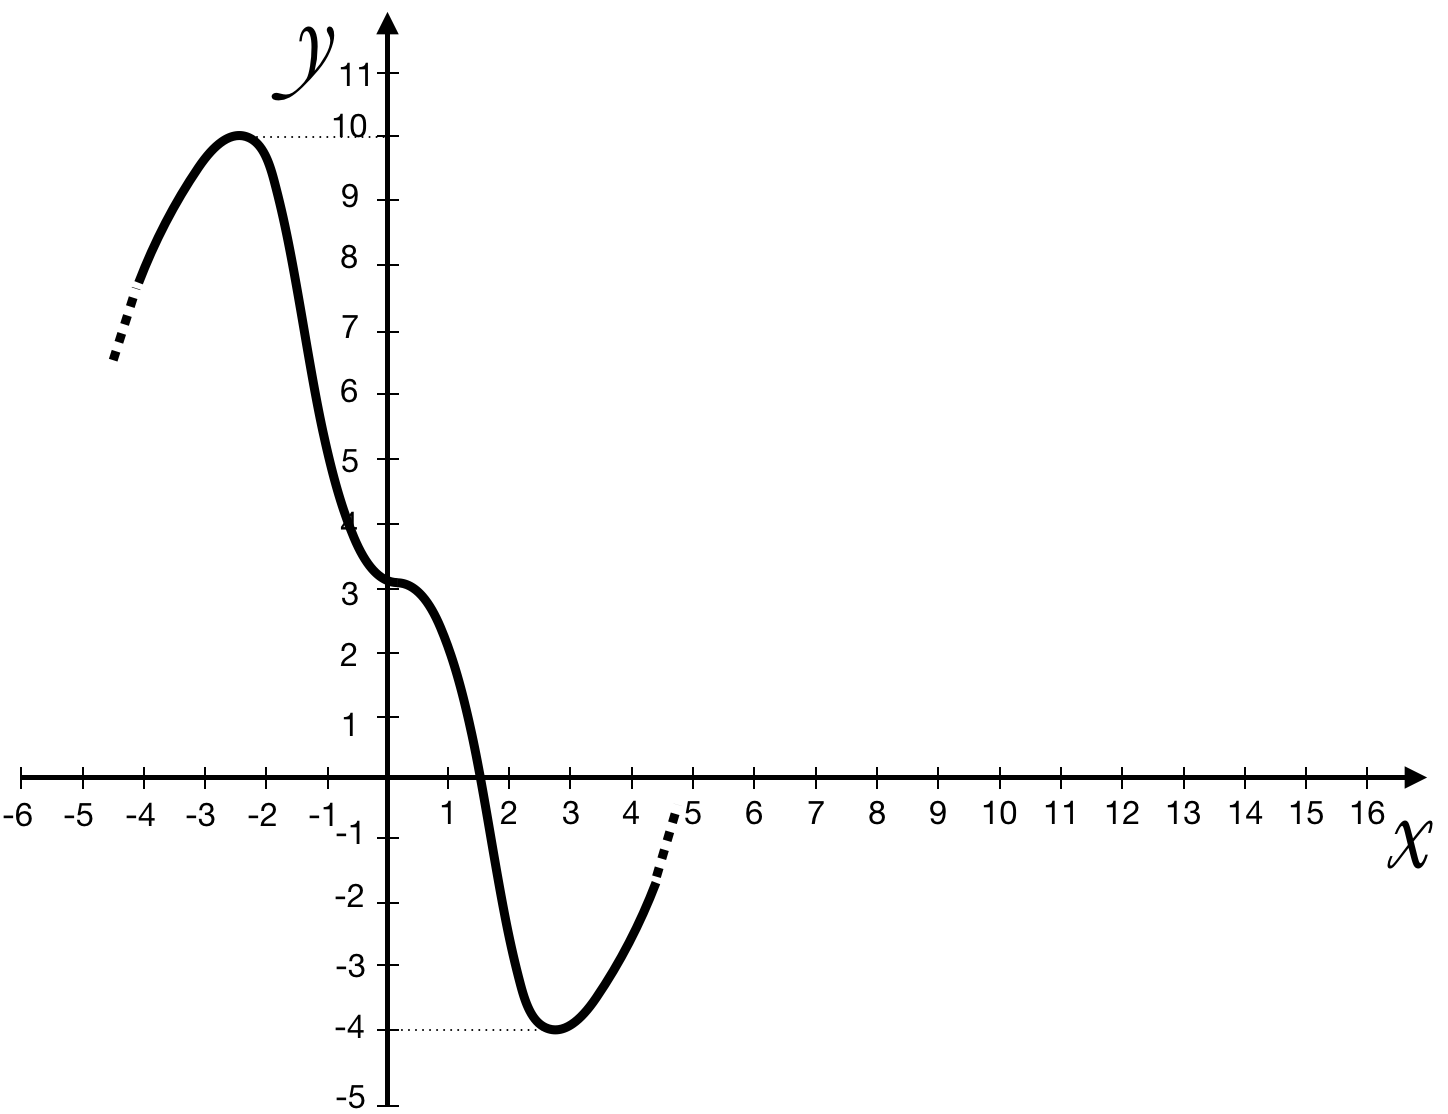
\includegraphics[width=0.45\textwidth]{img/funz_17c.png}   
  
\quad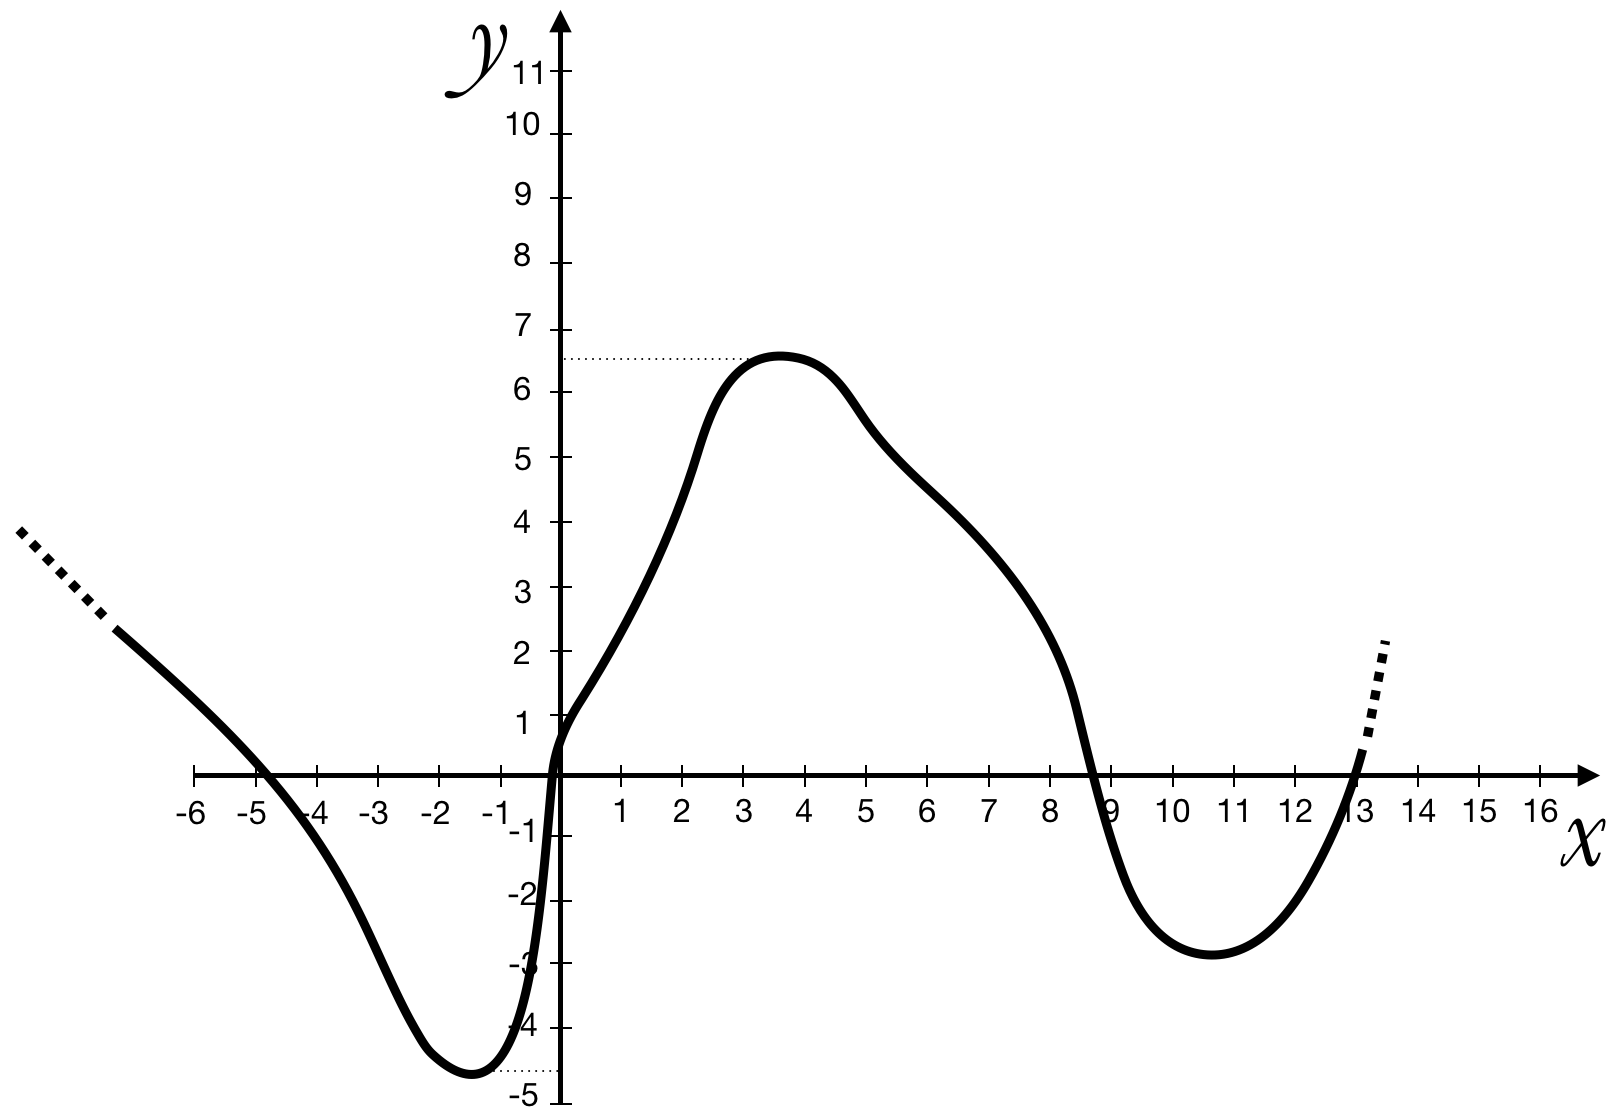
\includegraphics[width=0.45\textwidth]{img/funz_17d.png}
  %\caption{}
  %\label{fig:funz_14abc}
  \end{figure}
  \end{itemize}

\subsubsection*{1.2 La rappresentazione di una funzione}
%label{}
\begin{itemize}
  \item[1.4)] Immagina l'evoluzione della temperatura ora per ora nella 
città di Firenze, in una giornata di agosto, costruiscine la rappresentazione 
tabulare e quella grafica.
  \item[1.5)] Rappresenta graficamente le seguenti funzioni:
  \begin{itemize}
  \item[a)] $y=\sin2x$
  \item[b)] $y=3x+2$
  \item[c)] $y=x^2+2$
  \item[d)] $y=x^2+2x+3$
  \item[e)] $y=\log{(x+1)}$
  \item[f)] $y=e^x+2$
  \item[g)] $y=\frac{x+2}{2x-4}$
  \item[h)] $y=\sqrt{9-x}$
  \item[i)] $y=\sqrt{9-4x^2}$
  \item[l)] $y=\sqrt[3]{x}$
  \item[m)] $y=\vert x^2+4x+3\vert$
  \end{itemize}
\end{itemize}

\subsubsection*{1.3 Le proprietà di una funzione}
%label{}
\begin{itemize}
  \item[1.6)] Stabilisci se le seguenti funzioni, rappresentate 
graficamente, sono iniettive, suriettive o biunivoce, motivando la risposta.
  \begin{multicols}{2} 
  \begin{itemize}
  \item[(a)] $f:\mathbb{R}\to[0,+\infty[$
  \item[(c)] $f:\mathbb{R}\to]0,+\infty[$
  \item[(b)] $f:\mathbb{R}\to\mathbb{R}$
  \item[(d)] $f:\mathbb{R}\to\mathbb{R}$
  \end{itemize}
  \end{multicols}
  
  \begin{figure}[htpb!]
  \centering
  
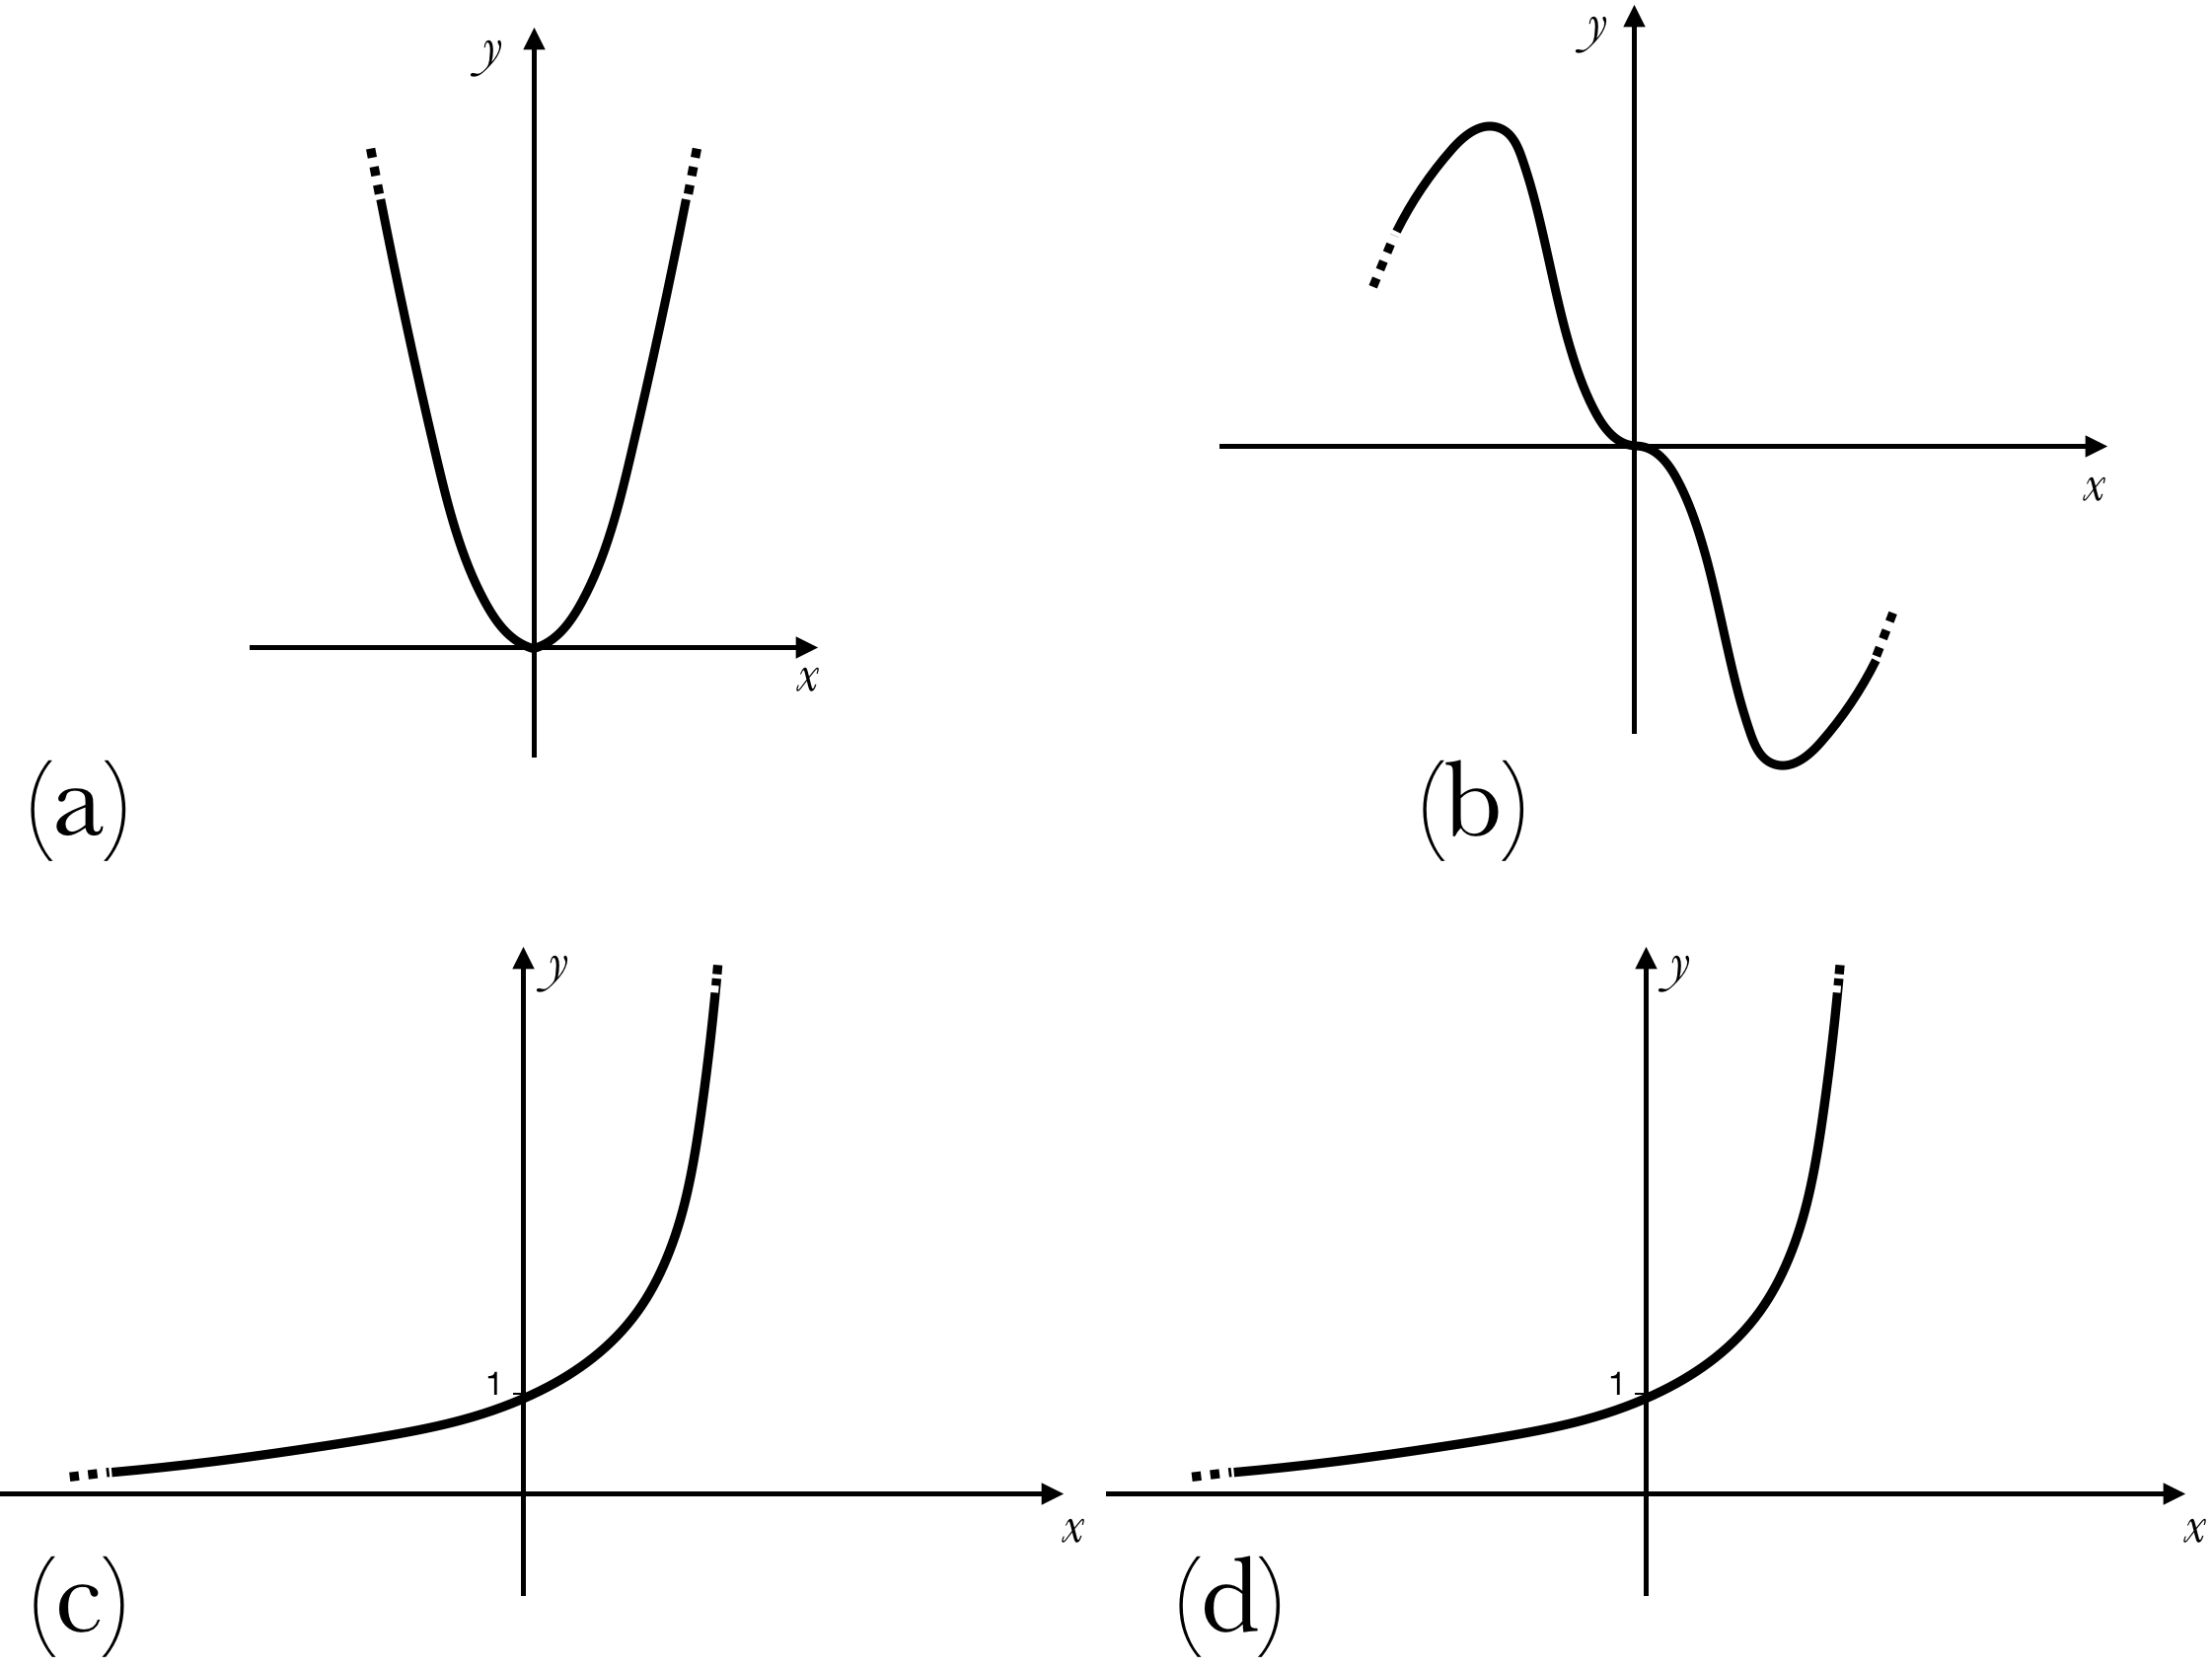
\includegraphics[width=0.65\textwidth]{img/funz_18.png}%\caption{}
  %\label{fig:funz_14abc}
  \end{figure}
\end{itemize}
\subsubsection*{1.4 Le caratteristiche di una funzione}
%label{}
\begin{itemize}
  \item[1.7)] Verifica se le seguenti funzioni sono pari o dispari.
  \begin{itemize}
  \item[a)] $y=2x+3$   \hfill   
  [né pari né dispari]
  \item[b)] $y=x^3+x$   \hfill  
   [dispari]
  \item[c)] $y=\frac{x^2+3}{x}$   \hfill  
  [dispari]
  \item[d)] $y=\frac{3x^4}{2+x^2} $   \hfill  
   [pari]
  \item[e)] $y=\tan{x}+\sin{x} $   \hfill   
 [dispari]
  \item[f)] $y= \log{(x-1)}$   \hfill   
[né pari né dispari]
  \end{itemize}
  
  \item[1.8)] Stabilisci se le seguenti funzioni sono periodiche, 
individuandone l'eventuale periodo.
  \begin{itemize}
  \item[a)] $y=\sin4x$   \hfill   
  [periodica $T=\frac{\pi}{2}$]
  \item[b)] $y=\tan2x$   \hfill   
  [periodica $T=\frac{\pi}{2}$]
  \item[c)] $y=\cos3x+1$   \hfill   
   [periodica $T=\frac{2\pi}{3}$]
  \item[d)] $y=\cos x+x $   \hfill  
   [non periodica]
  \item[e)] $y=\tan{\frac{x}{5}} $   \hfill   
   [periodica $T=5\pi$]
  \item[f)] $y= \sin(x+1)$   \hfill   
[periodica $T=2\pi$]
  \item[g)] $y= \sin x+1$   \hfill   
[periodica $T=2\pi$]
  \item[h)] $y= \sin x+x$   \hfill   
[non periodica]
  \item[i)] $y= \sin{\frac{x}{4}}$   \hfill   
  [periodica $T=8\pi$]
  \item[l)] $y= 2^{\sin{x}}$   \hfill   
[periodica $T=2\pi$]
  \item[m)] $y=x\cos x$   \hfill   [non 
periodica]
  \end{itemize}
\end{itemize}

\subsubsection*{1.5 La classificazione delle funzioni}
\begin{itemize}
  \item[1.9)] Classifica prima riguardo alle categorie algebrico o 
trascendente e poi rispetto alle categorie fratta o intera e razionale o 
irrazionale le seguenti funzioni.
  \begin{itemize}
  \item[a)] $y=\frac{x^2+x+2}{3x}$
  \item[b)] $y=\frac{4}{\sqrt{x-6}}$
  \item[c)] $y=e^x+x$; $y=\sqrt[3]{x^2+x}$
  \item[d)] $y=\frac{1}{3}\sqrt{3-x}$
  \item[e)] $y=\frac{\sin x}{4}$
  \item[f)] $y=\frac{x^2-4x}{3+\sqrt{2}}$
  \end{itemize}
\end{itemize}

\subsubsection*{1.6 Funzioni inverse, composte e uguali}
%label{}
\begin{itemize}
  \item[1.10)] Stabilisci se le seguenti funzioni sono invertibili 
senza restrizioni, giustificando la risposta.  \begin{itemize}
  \item[a)] $y=2x+3$ \hfill [invertibile]
  \item[b)] $y=x^2+9x+18$ \hfill [non invertibile]
  \item[c)] $y=e^x$ \hfill [invertibile]
  \item[d)] $y=\ln{x}$ \hfill [invertibile]
  \item[e)] $y=x^3+3x^2+x$ \hfill [non invertibile]
  \item[f)] $y=\sin x$ \hfill [non invertibile]
  \end{itemize}
  
  \item[1.11)] Determina l'inversa della funzione data, specificando il 
suo dominio.  
  \begin{itemize}
  \item[a)] $y=4x+3$ \hfill [$y=\frac{x-3}{4},\, 
D=\mathbb{R}$]
  \item[b)] $y=e^{2x}$ \hfill [$y=\frac{\ln x}{2},\, 
D=]0,+\infty[$]
  \item[c)] $y=x+1$ \hfill [$y=x-1,\, D=\mathbb{R}$]
  \item[d)] $y=\ln(x+1)$ \hfill [$y=e^x-1,\, 
D=\mathbb{R}$]
  \end{itemize}
  
  
  \item[1.12)] Date le funzioni $f(x)$ e $g(x)$ determina le 
espressioni analitiche di $f\circ g$ e di $g\circ f$.% non riesco a rendere 
ben leggibile questo esercizio
  \begin{itemize}
  \item[a)] $f(x)=\sqrt[3]{x+3}$  \\  $g(x)=\log_4{x}$  
\\  \hfill   $[(f\circ g)(x)=\sqrt[3]{\log_4{x+3}}; (g\circ 
f)(x)=\log_4{(\sqrt[3]{x+3})}]$
  
  \item[b)] $f(x)=3^x$  \\ $g(x)=x-5$   \\   
\hfill  $[(f\circ g)(x)=3^{x-5}; (g\circ f)(x)=3^x-5]$
  
  \item[c)] $f(x)=\cos3x$  \\ $g(x)=\sqrt{x^2+3}$  \\ 
   \hfill  $[(f\circ g)(x)=\cos{3\sqrt{x^2+3}}; (g\circ 
f)(x)=\sqrt{(\cos{3x})^2+3}]$
  
  \item[d)] $f(x)=x^2+3$ \\  $g(x)=2x+1$  \\  
\hfill  $[(f\circ g)(x)=(2x+1)^2+3=4x^2+4x+4; (g\circ 
f)(x)=2(x^2+3)+1=2x^2+7]$
  \end{itemize}
\end{itemize}
%mancano esercizi su limitatezza e monotonia (provvedo a creare dei grafici e 
semmai si aggiungono nei prossimi giorni...

%%%%%%%%%%%%%%%%%%%%%%%%%%%%%%%%%%%%%%%%%%%%%%%%%%%%%%
%%%%%%%%%%%%%%%%%%%%%TOPOLOGIA DELLA RETTA%%%%%%%%%%%%%%%%%%%

\chapter{Topologia della retta}
\section{La topologia della retta}
%label{}
Già dall'etimologia del termine, dal greco ``\emph{topos}'' che significa 
``luogo'', apprendiamo che il termine topologia indica lo studio ragionato 
dei luoghi. Nell'ambito dei nostri studi la topologia, o scienza dei luoghi, 
è quella branca della matematica che studia le proprietà geometriche delle 
figure piane e spaziali che restano inalterate eseguendo trasformazioni 
biunivoche. In particolare, con l'espressione topologia della retta si indica 
lo studio della retta come insieme di punti, approfondendo i concetti di 
vicinanza, lontananza e distanza tra di essi.\\

Il primo passo che facciamo è quello di identificare i numeri reali con i 
punti della retta: ad ognuno degli infiniti punti della retta facciamo 
corrispondere uno degli infiniti numeri dell'insieme $\mathbb{R}$. Ricordiamo 
infatti che entrambi sono insiemi ordinati e completi e possiamo costruire 
una corrispondenza biunivoca tra i loro elementi, fissando sulla retta 
un'origine e un verso di percorrenza, come ci consente di fare il postulato 
di ordinamento sulla retta.\\

Identificando i numeri reali con i punti della retta, possiamo definire la 
distanza tra due numeri $x$ e $y$ reali come la distanza $d(x, y)$ tra i 
punti che li rappresentano. Con $x$, $y\in\mathbb{R}$ la distanza è data da:
\begin{equation}
%\label{eq:}
  d(x,y)=\sqrt{(x-y)^2}=\vert x-y\vert
\end{equation}
ed ha le seguenti proprietà:
\begin{enumerate}
  \item $\forall x,\,y \in A,\,d(x,y)=d(y,x)$ cioè la distanza è 
simmetrica,
  \item $\forall x,\,y \in A,\,d(x,y)\geq0$,
  \item $d(x,y)=0\Leftrightarrow x=y$,
  \item $\forall x,\,y,\,z \in A,\,d(x,y)\leq d(x,z)+d(z,y)$ detta 
disuguaglianza triangolare.
\end{enumerate}

\section{Gli intervalli}
%label{}
  \begin{definizione}
Un \textsc{intervallo} è un sottoinsieme di $\mathbb{R}$, formato da tutti i 
reali compresi tra due estremi, finiti o infiniti.\\
\end{definizione}

Gli intervalli possono essere chiusi o aperti a seconda che gli estremi 
appartengano o meno all'intervallo.\\
Gli intervalli possono essere limitati se entrambi i loro estremi sono 
finiti: segmenti o illimitati se un estremo non è finito: semirette.

\textcolor{red}{TABELLA INTERVALLI da rifare o vedi quella a vol.2 pag.\dots}
\begin{figure}[htpb!]
  \centering
  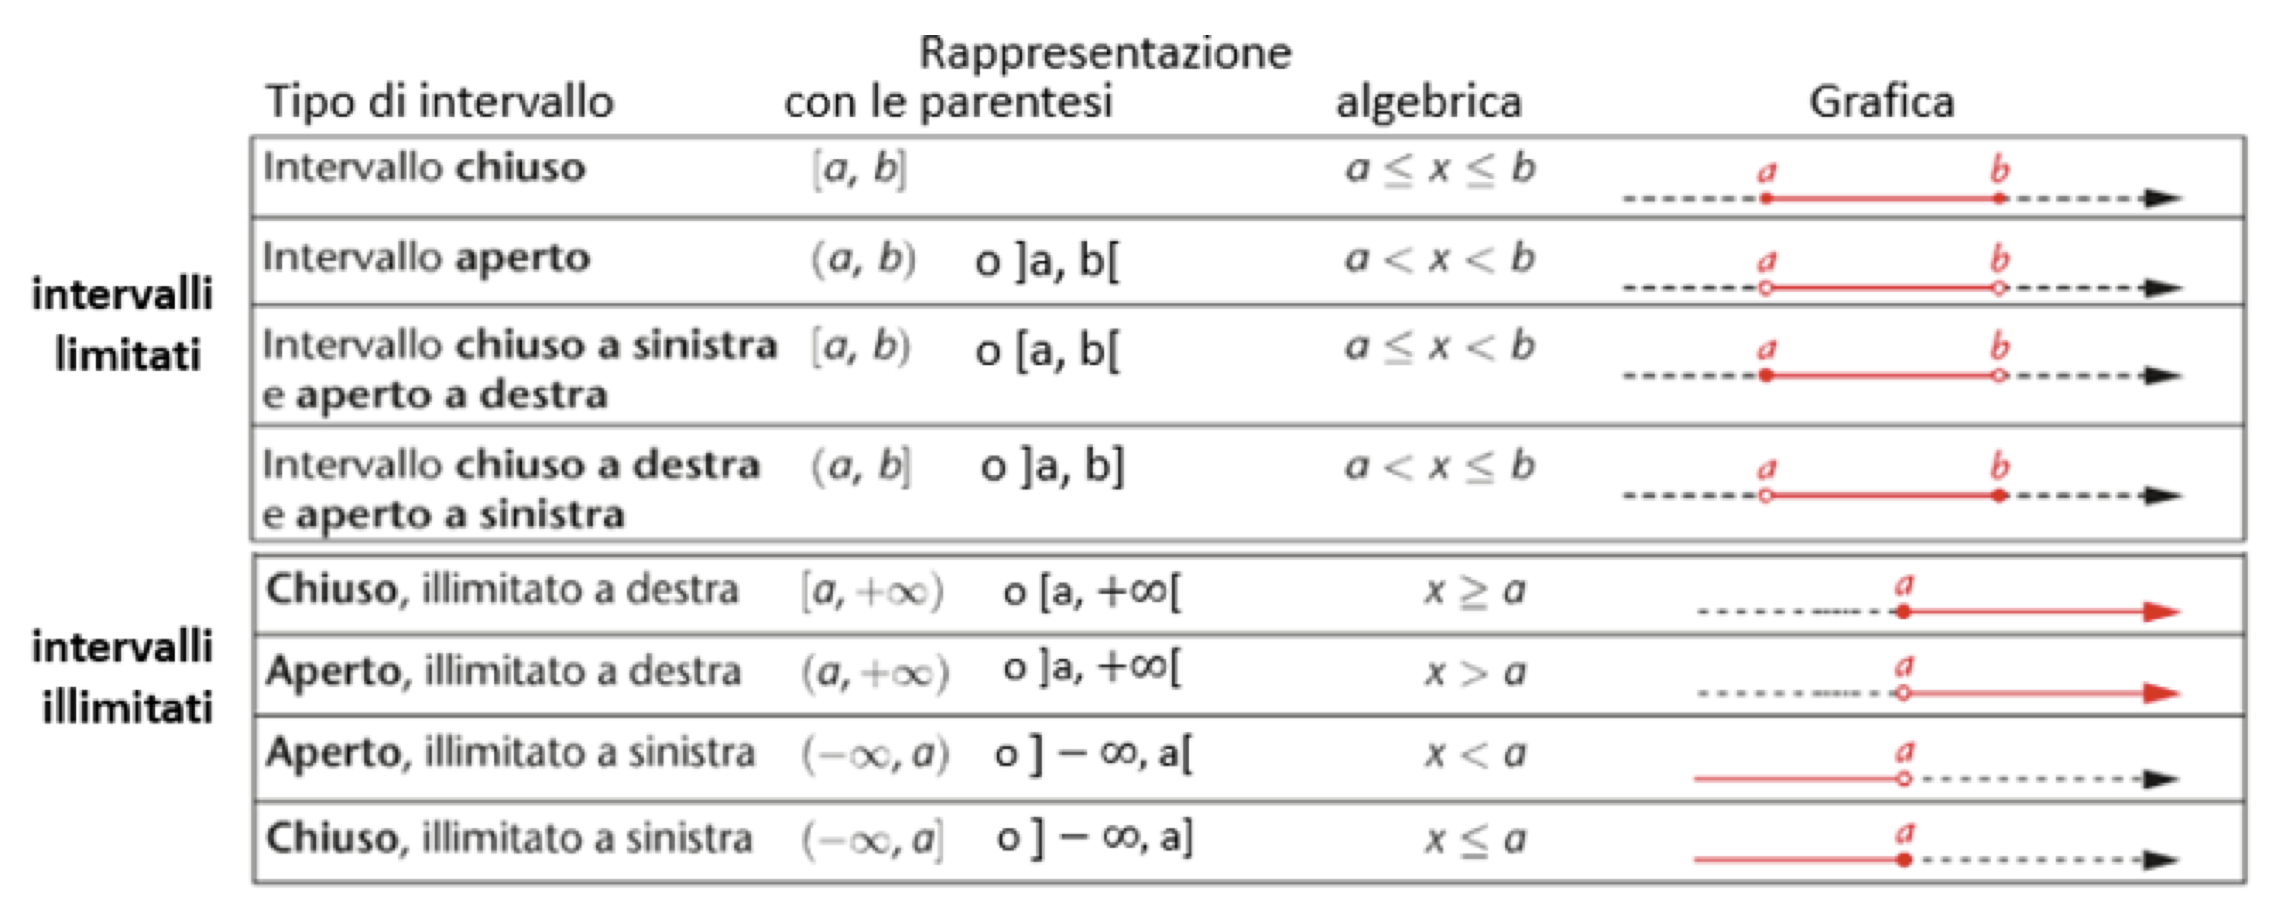
\includegraphics[width=1\textwidth]{img/top_tab.png}%\caption{}
  %\label{fig:funz_14abc}
\end{figure}




\begin{esempio} Intervalli finiti e infiniti: metodi di scrittura.
  \begin{itemize}
  \item[a)] L'insieme $\mathbb{R}$ si può scrivere come 
l'intervallo $]-\infty, +\infty[$\\
  \item[b)] L'insieme $\mathbb{R}-\{3\}$ si può indicare con 
l'intervallo $]-\infty, 3[\,\cup\,]3,+\infty[$\\
  \item[c)] L'insieme $\mathbb{R}-\{-2,3\}$ si può indicare con 
$]-\infty, -2[\,\cup\,]-2,3[\,\cup\,]3,+\infty[$\\
  \item[d)] L'insieme delle soluzioni della disequazione 
$x^2+3x>0$ si può scrivere come $]-\infty,-3[\,\cup\,]0,+\infty[$.\\
  \end{itemize}
\end{esempio}
  
Per quanto riguarda le operazioni tra intervalli evidenziamo che l'unione di 
intervalli aperti è un insieme aperto; l'intersezione di due intervalli 
aperti è un aperto. L'intersezione di intervalli chiusi è un intervallo 
chiuso; l'unione di un numero finito di intervalli chiusi è chiuso. Un 
intervallo $B$ è chiuso se il suo complementare è aperto.\\

Grazie alla corrispondenza tra numeri reali e punti di una retta, per 
indicare un elemento di un intervallo possiamo riferirci indifferentemente a 
un numero o un punto.

%
%
\section{Gli intorni}
%label{}
  \begin{definizione}
Si definisce intorno o intorno completo di un numero reale $x_0$, o punto 
$x_0$, un qualsiasi intervallo aperto contenente $x_0$.\\
  \end{definizione}

Rappresentiamo in simboli e graficamente un intorno
\begin{equation}
%\label{eq:}
I(x_0)=]x_0-\delta_1,x_0+\delta_2[
\end{equation}
con $\delta_1$ e $\delta_2$ reali positivi, cioè $\delta_1,\,\delta_2 \in 
\mathbb{R^+}$, o equivalentemente
\begin{equation}
%\label{eq:}
I(x_0)=\{x\in \mathbb{R}\,\vert\,x_0-\delta_1<x<x_0+\delta_2\}
\end{equation}
  \begin{figure}[htpb!]
  \centering
  
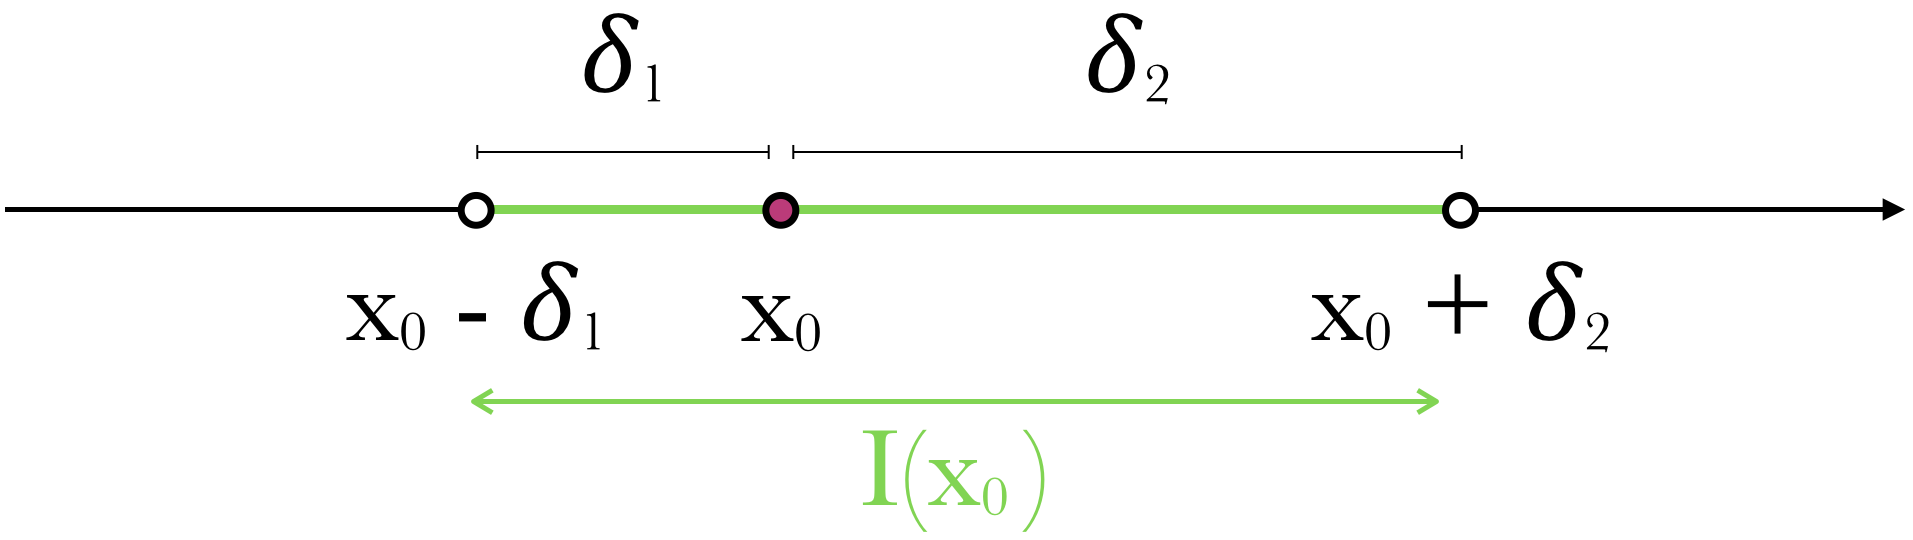
\includegraphics[width=0.5\textwidth]{img/top_1.png}%\caption{}
  %\label{fig:funz_14abc}
  \end{figure}
  
Da quanto visto risulta chiaro che per ogni numero reale, esistono infiniti 
intorni.\\
Per quanto riguarda le operazioni associabili agli intorni è da sottolineare 
che l'intersezione e l'unione di due o più intorni di $x_0$ sono ancora 
intorni di $x_0$.\\

\begin{figure}[htpb!]
\centering
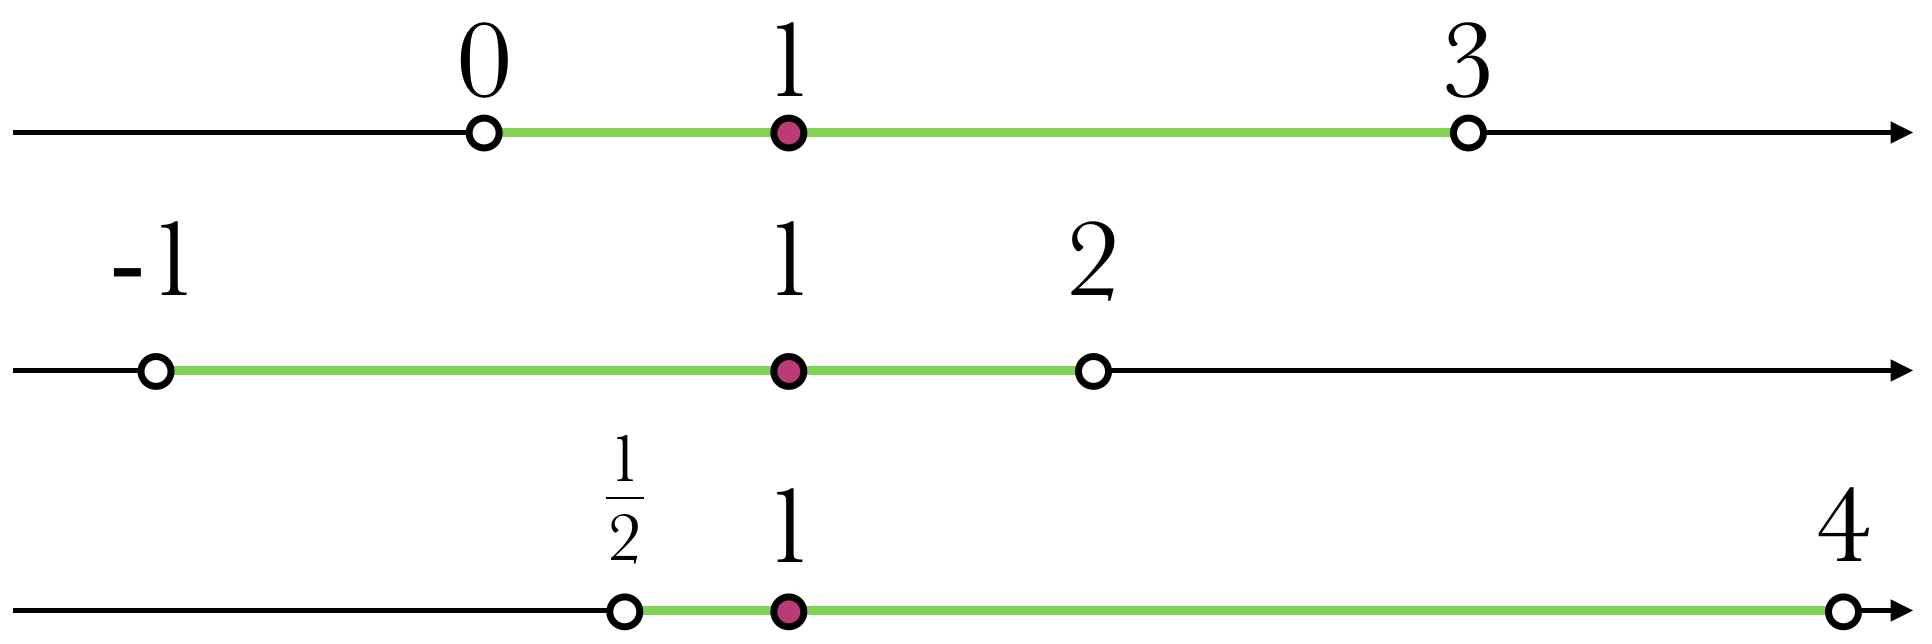
\includegraphics[width=0.5\textwidth]{img/top_7.png}%\caption{}
%\label{fig:funz_14abc}
  \end{figure}
  
Chiarito il concetto di intorno, introduciamo alcune particolari tipologie di 
intorno che renderanno più funzionale l'uso di questo concetto. Vedremo 
l'intorno circolare, l'intorno destro e l'intorno sinistro.\\

\begin{definizione}
  Dato un numero reale $x_0$ e un numero reale positivo $\delta$, si 
definisce \textsc{intorno circolare} di $x_0$, di raggio $\delta$, 
l'intervallo aperto $I_C(x_0)$ di centro $x_0$ e raggio $\delta$.\\
\end{definizione}

\begin{equation}
  I_C(x_0)=]x_0-\delta,\,x_0+\delta[
\end{equation}
o equivalentemente
 \begin{equation}
  I_C(x_0)=\{x\in \mathbb{R}\,\vert\,\vert x-x_0\vert<\delta\}
\end{equation}

\begin{figure}[htpb!]
  \centering
  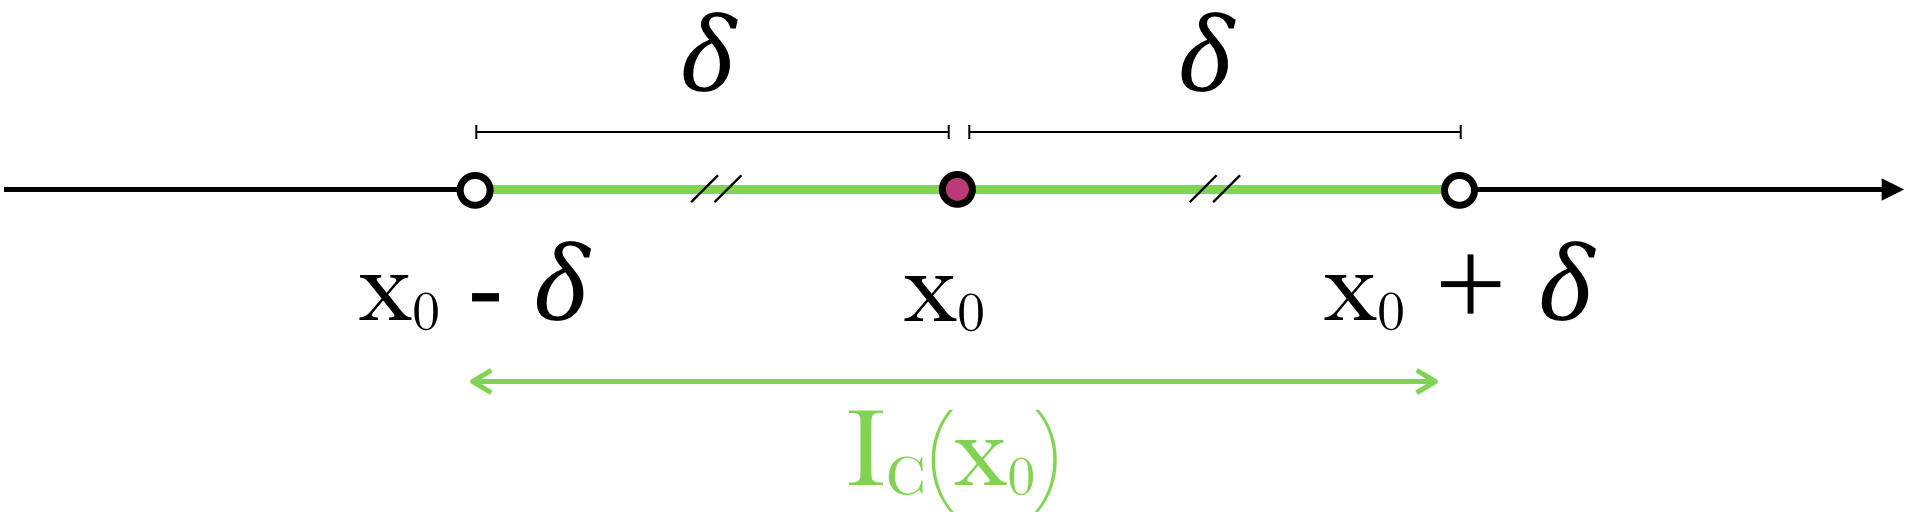
\includegraphics[width=0.5\textwidth]{img/top_2.png}%\caption{}
  %\label{fig:funz_14abc}
\end{figure}


\begin{definizione}
  Si dice intorno sinistro del numero reale $x_0$, $I_s(x_0)$ o 
$I^-(x_0)$, un qualsiasi intervallo aperto avente $x_0$ come estremo destro. 
$\delta\in\mathbb{R}$ è detta ampiezza.\\
\begin{equation}
  I_s(x_0)=]x_0-\delta,\,x_0[
\end{equation}
o equivalentemente
\begin{equation}
  I_s(x_0)=\{x\in \mathbb{R}\,\vert\, x_0-\delta < x<x_0\}
\end{equation}
\end{definizione}

\begin{figure}[htpb!]
  \centering
  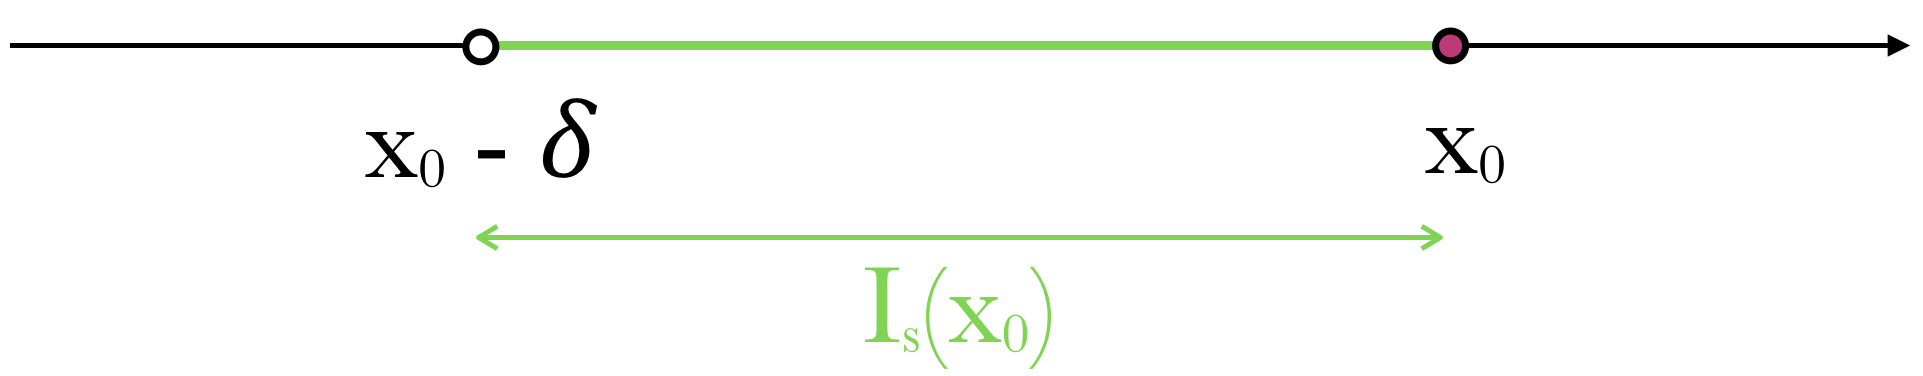
\includegraphics[width=0.5\textwidth]{img/top_3.png}%\caption{}
  %\label{fig:funz_14abc}
\end{figure}

\begin{definizione}
  Si dice intorno destro del numero reale $x_0$, $I_d(x_0)$ o 
$I^+(x_0)$, un qualsiasi intervallo aperto avente $x_0$ come estremo 
sinistro. $\delta\in\mathbb{R}$ è detta ampiezza.\\
\begin{equation}
  I_d(x_0)=]x_0,\,x_0+\delta[
\end{equation}
o equivalentemente
\begin{equation}
  I_d(x_0)=\{x\in \mathbb{R}\,\vert\, x_0 < x<x_0+\delta\}
\end{equation}
\end{definizione}

\begin{figure}[htpb!]
  \centering
  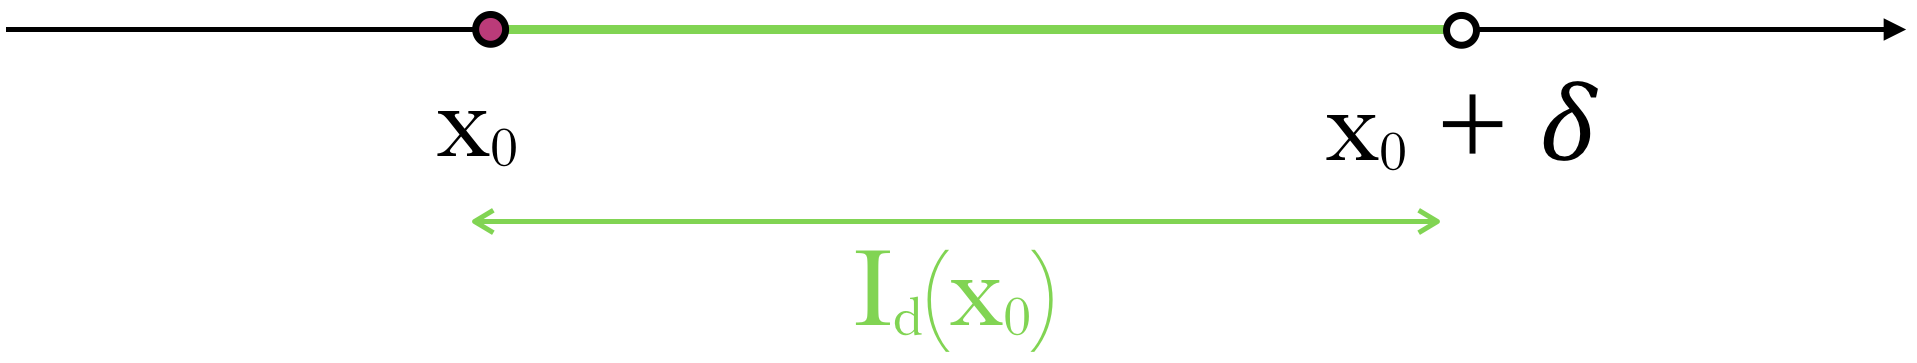
\includegraphics[width=0.5\textwidth]{img/top_4a.png}%\caption{}
  %\label{fig:funz_14abc}
\end{figure}

\begin{esempio} Intorni e intervalli.
\begin{itemize}
  \item[a)] L'intervallo $]-2, 9[$ è un intorno di $x_0=4$; rispetto a 
$x_0=4$ non sono intorni né $]5, 9[$ né $[3, 5]$.\\
  \item[b)] L'intervallo $]0, 6[$ è un intervallo circolare di $x_0=3$ 
di raggio $\delta=3$.\\
  \item[c)] L'intervallo $]\frac{4}{5},1[$ è un intorno sinistro di $1$ 
di ampiezza $\frac{1}{5}$. \\
\end{itemize}
\end{esempio}

\section{Insiemi limitati e illimitati}
%label{}
Consideriamo un insieme non vuoto $A\subset \mathbb{R}$. L'insieme A si dice 
superiormente limitato se esiste un numero $\alpha \in \mathbb{R}$ maggiore o 
uguale a tutti gli elementi di $A$, cioè $x\leq\alpha$ , $\forall x\in A$. 
Tale numero prende il nome di maggiorante, un insieme superiormente limitato 
ammette infiniti maggioranti. Se un insieme $A$ non è superiormente limitato 
si dice superiormente illimitato.\\
In simboli:\\

$A$ è \textsc{superiormente limitato} se 
\begin{equation}
  \exists \alpha\in\mathbb{R}\, \vert\, \forall x \in A,\,\alpha\geq x
\end{equation}
\\

$A$ è \textsc{superiormente illimitato} se 
\begin{equation}
  \forall M\in\mathbb{R},\, \exists x \in A\, \vert\,x> M
\end{equation}

Specularmente l'insieme $A$ si dice inferiormente limitato se esiste un 
numero $\beta\in \mathbb{R}$ minore o uguale a tutti gli elementi di $A$, 
cioè $x\geq\beta$ , $\forall x\in A$. Tale numero prende il nome di 
minorante, un insieme inferiormente limitato ammette infiniti minoranti. Se 
un insieme $A$ non è inferiormente limitato si dice inferiormente illimitato.
In simboli:\\

$A$ è \textsc{inferiormente limitato} se 
\begin{equation}
  \exists \beta\in\mathbb{R}\, \vert\, \forall x \in A,\,\beta\leq x
\end{equation}
\\

$A$ è \textsc{inferiormente illimitato} se 
\begin{equation}
  \forall m\in\mathbb{R},\, \exists x \in A\, \vert\,x< m
\end{equation}
Infine, completiamo la trattazione appena fatta notando che l'insieme $A$ si 
dice limitato se è sia inferiormente limitato che superiormente limitato, 
esiste cioè un intervallo limitato che lo contiene. Un insieme illimitato 
superiormente e inferiormente si dice illimitato.\\

\begin{esempio} Limitatezza/illimitatezza di insiemi, maggioranti e minoranti.
\begin{itemize}
  \item[a)] L'insieme $A=]-\infty,4[ \cup [8,15]$ è superiormente 
limitato, perché tutti i suoi elementi sono minori o uguali a 15. 15 è un 
maggiorante, ma anche 16, 20 e 204 lo sono. $A$ è, poi, inferiormente 
illimitato.\\
  \item[b)] L'insieme $B=\{5\}\cup]9,+\infty[$ è inferiormente limitato 
e tutti i numeri minori o uguali a 5 sono minoranti; l'insieme è 
superiormente illimitato.\\

  \item[c)] L'insieme $C=\{x\in\mathbb{R}\vert 
x=\frac{1}{n},\,n\in\mathbb{N}-\{0\}\}=\{1,\frac{1}{2},\frac{1}{3}
,\dots\}$ è limitato, ha 1 come maggiorante e 0 come minorante. Altri 
minoranti ad esempio sono $-3$, $-5$ ecc, altri maggioranti 5, 8 ecc.\\

  \item[d)] L'insieme $D=]3,5]\cup[7,9[$ ammette 2 come minorante e 10 
come maggiorante, quindi è sia inferiormente che superiormente limitato: $D$ 
è limitato.\\

  \item[e)] L'insieme $\mathbb{Q}$ non ammette né minoranti né 
maggioranti, quindi non è non è limitato né inferiormente né superiormente.\\
\end{itemize}
\end{esempio}

Avendo introdotto gli insiemi illimitati possiamo ora parlare degli intorni 
di infinito. Anche se $+\infty$ e $-\infty$ non sono numeri reali è utile 
introdurne gli intorni.\\

\begin{definizione}
  Dati $a,\,b\in\mathbb{R}$ con $a<b$, definiamo \textsc{intorno di 
meno infinito} un qualsiasi intervallo illimitato a sinistra e aperto a destra
\begin{equation}
  I(-\infty)=]-\infty,a[=\{x\in\mathbb{R}\vert x<a\}
\end{equation}
\end{definizione}

\begin{figure}[htpb!]
  \centering
  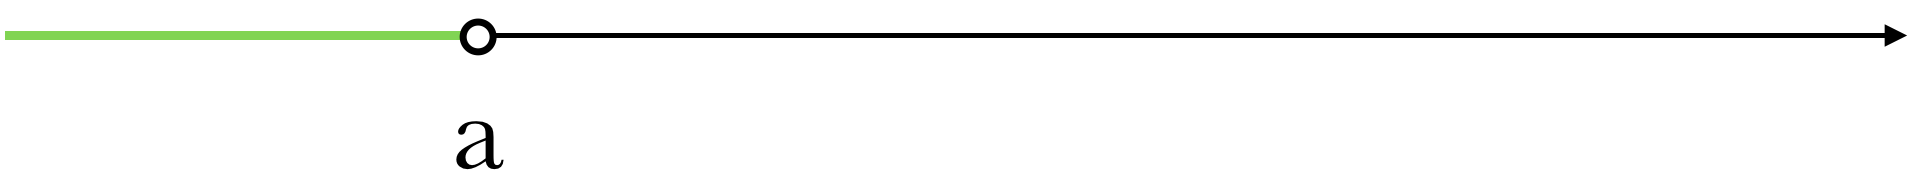
\includegraphics[width=0.5\textwidth]{img/top_4.png}%\caption{}
  %\label{fig:funz_14abc}
\end{figure}


\begin{definizione}
  Dati $a,\,b\in\mathbb{R}$ con $a<b$, definiamo \textsc{intorno di più 
infinito} un qualsiasi intervallo illimitato a destra e aperto a sinistra
\begin{equation}
  I(+\infty)=]b,+\infty[=\{x\in\mathbb{R}\vert x>b\}
\end{equation}
\end{definizione}

\begin{figure}[htpb!]
  \centering
  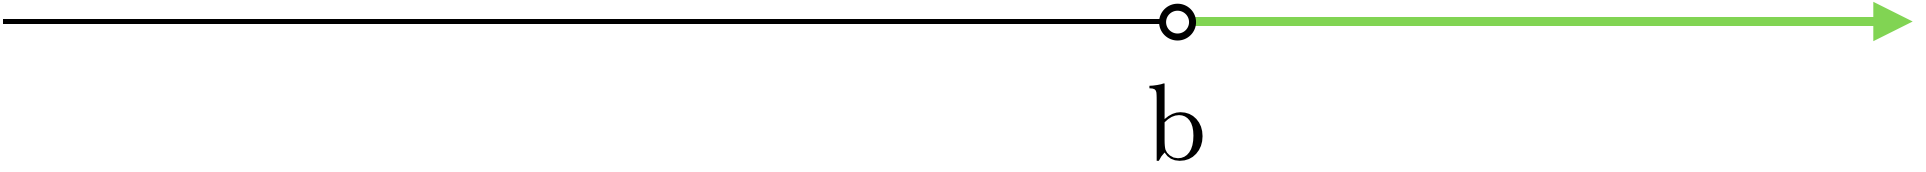
\includegraphics[width=0.5\textwidth]{img/top_5.png}%\caption{}
  %\label{fig:funz_14abc}
\end{figure}

\begin{definizione}
  Dati $a,\,b\in\mathbb{R}$ con $a<b$, definiamo \textsc{intorno di 
infinito} l'unione tra un intorno di $-\infty$  e un intorno di $+\infty$ 
\begin{equation}
  I(\infty)=I(-\infty)\cup I(+\infty)=\{x\in\mathbb{R}\vert x<a \lor 
x>b\}
\end{equation}
e \textsc{l'intorno circolare di infinito}, dove $c\in\mathbb{R}^+$ come
\begin{equation}
  I_c(\infty)=]-\infty,-c[\cup]c,+\infty[
\end{equation}
\end{definizione}

\begin{figure}[htpb!]
  \centering
  
\includegraphics[width=0.5\textwidth]{img/top_6.png}%\caption{}
  %\label{fig:funz_14abc}
\end{figure}


\begin{esempio} Scrivere gli intervalli risultato di una disequazione come 
intorni di infiniti.
\begin{itemize}
  \item[a)] Le soluzioni della disequazione $x+4>0$ formano un intorno 
di $+\infty$.  Soluzioni: $x>-4$, $I(+\infty)=]-4, +\infty[$.\\
  \item[b)] Le soluzioni della disequazione $x^2+5x+6>0$ formano un 
intorno di infinito. Soluzioni: $-3<x\lor x>-2$, $I(\infty)=]-\infty, -3[ 
\cup]-2, +\infty[$.\\
  \item[c)] Consideriamo la disequazione $\vert x\vert>3$, le soluzioni 
forniscono un esempio di intorno circolare di $\infty$ che è 
$I_c(\infty)=]-\infty,-3[\cup]3,+\infty[$.
\end{itemize} 
\end{esempio}

\section{Massimi, minimi ed estremi}
%label{}
Ragioniamo ora su quanto appena visto, nel precedente paragrafo. Se un 
insieme $A$ è superiormente limitato ha infiniti maggioranti; si può allora 
individuare un insieme di maggioranti, tra i quali non è identificabile un 
maggiorante più grande di tutti, mentre possiamo pensare a un maggiorante più 
piccolo di tutti.\\

Questo maggiorante viene chiamato estremo superiore di $A$, se tale punto è 
anche compreso in $A$ prende il nome di massimo. Chiaramente potremmo fare un 
discorso analogo per i minoranti, individuando il maggiore tra di essi, detto 
estremo inferiore. Se l'estremo inferiore appartiene all'insieme che si sta 
studiando, prende il nome di minimo. Entriamo nel merito delle definizioni.\\

\begin{definizione}
  Un numero reale $M$ si dice massimo di $A$, $\max{A}$, se appartiene 
ad $A$ ed è un maggiorante di $A$.\\
\end{definizione}

\begin{definizione}
  Un numero reale $m$ si dice minimo di $A$, $\min{A}$, se appartiene 
ad $A$ ed è un minorante di A.\\
\end{definizione}

\begin{definizione}
  Si definisce $S$ estremo superiore di $A$, $\sup{A}$, se esiste, il 
minimo dell'insieme dei maggioranti.\\
\end{definizione}

\begin{definizione}
  Si definisce $s$ estremo inferiore di $A$, $\inf{A}$, se esiste, il 
massimo dell'insieme dei minoranti.\\
\end{definizione}

\begin{esempio}Studiamo i massimi e i minimi dei seguenti intervalli.\\
Consideriamo l'intervallo chiuso $[0,2]$, esso presenta un minimo in 0 e un 
massimo in 2, se prendiamo invece l'intervallo aperto $]0,2[$ esso non avrà 
né massimo né minimo, perché né 0 né 1 appartengono all'insieme. Risulta 
chiaro quindi che nell'intervallo aperto solo a destra $[0,2[$ sarà presente 
un minimo, cioè 0, ma non un massimo.\\
\end{esempio}

\begin{esempio}Studiamo gli estremi superiore ed inferiore dei seguenti 
intervalli.\\
Consideriamo l'intervallo $A=]1, 5]$, aperto a sinistra e chiuso a destra. 
L'intervallo ha un estremo inferiore in 1, infatti questo valore è il massimo 
dei minoranti, 1 però non è minimo in quanto non compreso in $A$. Lo stesso 
intervallo ha estremo superiore in 5, che, essendo compreso, è anche massimo. 
Notiamo che l'insieme dei maggioranti di $A$ è infatti l'insieme 
$\{x\in\mathbb{R}\vert x\geq5\}$, l'insieme dei minoranti è 
$\{x\in\mathbb{R}\vert x\leq1\}$.\\
Consideriamo ora l'intervallo $B=\{x\in\mathbb{R}\vert x<3\}$, non essendo 
inferiormente limitato $B$ non presenta né estremo inferiore né minimo. 
L'estremo superiore di $B$ è 3, che non essendo compreso non è massimo.\\
\end{esempio}

Soffermiamoci ancora sui concetti di $\sup$, estremo superiore, e di $\inf$, 
estremo inferiore, enunciando la seguente proprietà che precisa l'esistenza e 
l'unicità di $\sup$ e $\inf$ negli insiemi limitati:\\

Sia $A\subset\mathbb{R}$, non vuoto:
\begin{itemize}
  \item se $A$ è superiormente limitato allora esiste in $\mathbb{R}$ 
l'estremo superiore di $A$ $\sup{A}$ ed è unico.
  \item se $A$ è inferiormente limitato allora esiste in $\mathbb{R}$ 
l'estremo inferiore di $A$ $\inf{A}$ ed è unico.
\end{itemize}

\section{I punti di accumulazione}
%label{}
Pensiamo ad un intervallo dato dall'insieme $A=]3, 5[$ e ad un insieme fatto 
invece di singoli punti $B=\{2,3,4,5,6\}$ e ragioniamo sul fatto che nel 
primo insieme preso un qualsiasi punto ad esempio 4, ci sarà sempre un 
intorno di 4 che contiene altri punti di $A$; anche se prendiamo in 
considerazione 3, che a dire la verità, non fa parte di A, potrei prendere un 
intorno qualsiasi di 3 e verificare che vi è almeno un punto di $A$. Questa 
riflessione non si può applicare invece all'insieme $B$, perché se prendo un 
intorno di 3, nella fattispecie un intorno circolare di raggio $\frac{1}{2}$, 
in quell'intorno non sono compresi altri punti di $B$ perché gli elementi di 
$B$ più vicini a 3 sono 2 e 4.\\

Stiamo provando ad illustrare il concetto di contiguità che gli elementi di 
un insieme mostrano, mentre gli elementi di altri insiemi non mostrano. Siamo 
pronti per la definizione di punto di accumulazione.\\

\begin{definizione}
  Dato $A$ sottoinsieme di $\mathbb{R}$, definiamo $x_0$ punto di 
accumulazione di $A$ se ogni intorno di $x_0$ contiene almeno un elemento di 
$A$ diverso da $x_0$.
\begin{itemize}
  \item[$\rhd$] Un punto di accumulazione di un insieme può appartenere 
o non appartenere all'insieme stesso.
  \item[$\rhd$]   Si può dimostrare che se $x_0$ è punto di 
accumulazione di $A$, in ogni intorno di $x_0$ devono cadere infiniti 
elementi di $A$. Consegue da questo che un insieme finito è privo di punti di 
accumulazione.
  \item[$\rhd$] L'insieme costituito dai punti di accumulazione di $A$ 
si chiama insieme derivato: $Der A$.
\end{itemize}
\end{definizione}

Come abbiamo visto nell'introduzione a questo paragrafo non tutti i punti si 
comportano come 4 per l'insieme $A$, cioè sono di accumulazione; possono 
esserci anche punti che si comportano come 3, per l'insieme $B$, cioè sono 
isolati.\\

\begin{definizione}
  Un punto $x_0$ che appartiene ad $A$ ma non è di accumulazione per $A$ 
si dice isolato. $x_0\in A$ è un punto isolato di $A$ se esiste almeno un 
intorno $I$ di $x_0$ che non contiene altri elementi di $A$ diversi da 
$x_0$.\\
\end{definizione}

Un sottoinsieme $A$ di $\mathbb{R}$ si dice \textsc{discreto} se non contiene 
nessuno dei suoi punti di accumulazione. $A$ è discreto se e solo se è 
formato da punti isolati.\\
Un insieme $B$ si dice \textsc{denso} in sé se ogni suo punto è di 
accumulazione per esso, cioè se $B\subseteq Der B$.\\

Dato $X\subset \mathbb{R}$ classifichiamo i punti di $\mathbb{R}$ 
relativamente ad $X$:
\begin{itemize}
  \item I punti interni di $X$ sono quelli che appartengono a $X$ e 
possiedono un intorno interamente contenuto in $X$.
  \item   I punti esterni ad $X$ sono quelli che non appartengono a $X$ 
e possiedono un intorno completamente disgiunto da $X$.
  \item   I punti di frontiera di $X$ hanno la proprietà che ogni loro 
intorno contiene sia punti di $X$ che punti che non appartengono a $X$.
\end{itemize}

\begin{esempio}
Relazione fra l'appartenenza di un punto all'insieme e l'essere di 
accumulazione per quell'insieme.
\begin{itemize}
  \item[a)] $x_0$ appartiene ad $A$, $x_0$ è di accumulazione per $A$\\
 $\longrightarrow$ $A=]4,8[$, $x_0=5\rightarrow x_0\in A$ ed è di 
accumulazione.
  \item[b)]  $x_0$ non appartiene ad $A$, $x_0$ è di accumulazione per 
$A$\\
 $\longrightarrow$ $A=]4,8[$, $x_0=4\rightarrow x_0\notin A$ ed è di 
accumulazione.
  \item[c)]  $x_0$ non appartiene ad $A$, $x_0$ non è di accumulazione 
per $A$\\
 $\longrightarrow$ $A=]4,8[$, $x_0=2\rightarrow x_0\notin A$ e non è di 
accumulazione.
  \item[d)] $x_0$ appartiene ad $A$, $x_0$ non è di accumulazione per 
$A$\\
  $\longrightarrow$ $A=]4,8[$, $x_0=9\rightarrow x_0\in A$ e non 
è di accumulazione.
\end{itemize}
\end{esempio}

\begin{esempio}
Studio dei punti di accumulazione.
\begin{itemize}
  \item[a)] L'insieme $A=\{ 5,6,7,8\}$ essendo finito non ha punti di 
accumulazione.
  \item[b)] Consideriamo l'insieme $C=]1,6[\,\cup\,]6,8]$
  \begin{itemize}
  \item $C$ non ha minimo, il massimo è 8;
  \item L'estermo inferiore è 1, l'estremo superiore 8;
  \item L'insieme dei minoranti è $]-\infty,1]$ ;
  \item L'insieme dei maggioranti è $[8,+\infty[$ ;
  \item 1 e 6 sono di accumulazione per $C$ ma non 
appartengono a $C$;
  \item 8 è di accumulazione per $C$ e appartiene a $C$;
  \item Tutti i numeri compresi tra 1 e 8 sono di 
accumulazione per $C$;
  \end{itemize}
  \item[c)] Analizziamo l'insieme $\mathbb{Q}$ che sappiamo essere 
denso. Ogni numero irrazionale è di accumulazione per $\mathbb{Q}$, ma anche 
ogni numero razionale è di accumulazione per $\mathbb{Q}$. Tutti i numeri 
reali sono di accumulazione per $\mathbb{Q}$, $\mathbb{R}$ è l'insieme 
derivato di $\mathbb{Q}$.\\
  \item[d)] $$A=\biggl\{ x\in\mathbb{R} \vert x=\frac{1}{n}, 
\,\text{con}\,\, n\in\mathbb{N},\,n\geq1 \biggr\}$$
Al crescere di $n$, gli elementi tendono a 0, che è punto di accumulazione: 
in ogni intorno di 0 c'è almeno un punto di $A$. Ci sono tra gli elementi di 
$A$ o tra i numeri reali altri punti di accumulazione per $A$, oltre a 0? No, 
non ci sono.\\
\end{itemize}
\end{esempio}
\newpage
\section{Esercizi}
%label{}
  \subsection{Esercizi dei singoli paragrafi}
  %label{}
  \subsubsection*{2.1 La topologia della retta}
  %label{}
  \begin{itemize}
  \item[2.1)] Rispondi alle seguenti domande, 
nella maniera più dettagliata e precisa possibile.
  \begin{itemize}
  \item[a)] Cosa si intende per 
topologia della retta?
  \item [b)] Qual è la 
principale identificazione che si fa nello studio della topologia della retta?
  \item[c)] Descrivi cosa si 
intende per distanza tra punti.
  \item[d)] Enuncia almeno tre 
proprietà della distanza, spiegandone il significato.
  \end{itemize}   
  \end{itemize}
  \subsubsection*{2.2 Gli intervalli}
  %label{}
  \begin{itemize}
  \item[2.2)] Data la rappresentazione algebrica 
dei seguenti intervalli esprimili sia graficamente che mediante le parentesi:
$$a)\, x\geq2\,\,\, \,\,\, \,\,\, \,\,\, b)\, 3<x<5  \,\,\,\,\,\, \,\,\,   
c)\, 4<x<7,\, x\neq5  \,\,\,  \,\,\, \,\,\,  d)\, x<-3 $$
$$ e) \, \frac{1}{2}<x\leq2 \,\,\, \,\,\,  \,\,\,  f)\, \frac{3}{4}\leq 
x\leq3\,\,\, \,\,\, \,\,\,  g)\, x\leq2\land x\geq4$$

  \item[2.3)] Risolvi le seguenti disequazioni, 
trovandone l'intervallo di soluzione
  \begin{itemize}
  \item[a)] $x^2+2>0$  
   \hfill  [ $]-\infty,+\infty[$ ]
  \item[b)] $3x^2-8x\geq0$   
   \hfill   [ $]-\infty,0]\,\cup\,[\frac{8}{3},+\infty[$ 
 ]
  \item[c)] $6x^2-5x+1>0$  
  \hfill   [ $]-\infty, 
\frac{1}{3}[\,\cup\,]\frac{1}{2}, +\infty[$  ]
  \item[d)] $-3x^2-2>0$  
  \hfill   [$\emptyset$]
  \item[e)] $x(x-2)(2x+3)<0$   
   \hfill   [ $]-\infty, -\frac{3}{2}[\,\cup\, ]0, 2[$ ]
  \item[f)] 
$\frac{2x+5}{x-3}\geq0$   \hfill   [ $ 
]-\infty,-\frac{5}{2}]\,\cup\,]3,+\infty[$ ]
  \item[g)] 
$\frac{(x+2)^2}{3-x}>0$  \hfill   [ $ ]-\infty, 
-2[\,\cup\,]-2, 3[$ ]
  \end{itemize}
  \end{itemize}   
  \subsubsection*{2.3 Gli intorni}
  %label{}
  \begin{itemize}
  \item[2.4)] Ricordando le diverse tipologie di 
intorno classifica gli intorni seguenti rispetto al punto indicato, 
determinando ampiezze e raggi.
  \begin{itemize}
  \item[a)] $]3, 7[$ rispetto a 
$x_0=5$   \hfill   [circolare di raggio 2]
  \item[b)] $]2, 5[$ rispetto a 
$x_0=2$   \hfill  [destro di ampiezza 3]
  \item[c)] $]3, 4[$ rispetto a 
$x_0=4$  \hfill  [sinistro di ampiezza 1]
  \item[d)] $]1/4, 3/4[$ 
rispetto a $x_0=\frac{1}{2}$   \hfill  [circolare di ampiezza $\frac{1}{4}$]
  \item[e)] $]3, 7/2[$ rispetto 
a $x_0=3$   \hfill  [destro di ampiezza $\frac{1}{2}$] 
  \item[f)] $]\frac{2}{5}, 2[$ 
rispetto a $x_0=2$  \hfill   [sinistro di ampiezza $\frac{8}{5}$]
  \item[g)] $]-\frac{8}{5}, 
-\frac{4}{5}[$ rispetto a $x_0= -\frac{6}{5}$   \hfill [circolare di ampiezza 
$\frac{2}{5}$]
  \end{itemize}
  \end{itemize}
  \subsubsection*{2.4 Insiemi limitati e illimitati}
  %label{}
  \begin{itemize}
  \item[2.5)]  Stabilisci se i seguenti insiemi 
sono superiormente/inferiormente limitati/illimitati
$$a)\, [3, 5]  \,\,\, \,\,\,   b)\, ]3, 5[  \,\,\, \,\,\,   c)\, ]-\infty, 
\frac{1}{2}[   \,\,\, \,\,\,  $$ 
  $$d)\,]-\infty, 3[\,\cup\,\{6\}  \,\,\,\,\,\,  e)\,  ]-\infty, 
-2]\,\cup\,[2, +\infty[ \,\,\,\,\,\,  f)\, [\sqrt{2}, +\infty[$$
  \end{itemize}
  \subsubsection*{2.5 Massimi minimi ed estremi}
  %label{}
  \begin{itemize}
  \item[2.6)] Individua, se esistono, massimi, 
minimi, estremi superiori ed inferiori dei seguenti intervalli
  \begin{itemize}
  \item[a)]  $A=[1.5] $  
\hfill   [$\min{A}=1$, $\inf{A}=1$, $\max{A}=5$, $\sup{A}=5$]
  \item[b)] $A=]3,6]$   \hfill   
  [$\min{A}$ non esiste, $\inf{A}=3$, $\max{A}=6$, $\sup{A}=6$]
  \item[c)] $A=]-2,+\infty[$  
\hfill   [$\min{A}$ non esiste, $\inf{A}=-2$, $\max$ e $\sup$ non esistono]
  \item[d)] 
$A=[2,5[\,\cup\,]6,8[$  \hfill [$\min{A}=2$, $\inf{A}=2$, $\max{A}$ non 
esiste, $\sup{A}=8$]
  \item[e)] $A=]-\infty, 4]$   
\hfill   [$\min$ e $\inf$ non esistono, $\max{A}=4$, $\sup{A}=4$]
  \end{itemize}
  \end{itemize}
  \subsubsection*{2.6 I punti di accumulazione}
  %label{}
  \begin{itemize}
  \item[2.7)] Stabilisci se i punti indicati 
sono di accumulazione per gli insiemi assegnati
  \begin{itemize}
  \item[a)]  $A=[3, 7]$ \hfill  
$x_0=2$, $x_1=3$, $x_2=5$
  \item[b)] $A=]4, 9[$  \hfill  
$x_0=4$, $x_1=5$, $x_2=11$
  \item[c)] $A=\{2,3,4,5\}$  
\hfill  $x_0=2$, $x_1=3$, $x_2=5$
  \item[d)] $\mathbb{R}$ \hfill  
$x_0=-2$, $x_1=0$, $x_2=\sqrt{3}$
  \item[e)] $\mathbb{N}$ \hfill  
$x_0=1$, $x_1=3$, $x_2=15$
  \item[f)] 
$A=\{x\in\mathbb{R}\vert x=\frac{3n}{n+1},\,n\in\mathbb{N}\}$ \hfill  
$x_0=3$, $x_1=4$ 
  \end{itemize}
  \end{itemize}
  










